%% USPSC-Cap2-DesenvolvimentoTutorial.tex 

% ---
% Este cap\'{\i}tulo, utilizado por diferentes exemplos do abnTeX2, ilustra o uso de
% comandos do abnTeX2 e de LaTeX.
% ---

\chapter{Desenvolvimento}\label{cap_exemplos}
Este cap\'{\i}tulo \'e parte principal do trabalho acad\^emico e deve conter a exposi\c{c}\~ao ordenada e detalhada do assunto. Divide-se em se\c{c}\~oes e subse\c{c}\~oes, em conformidade com a abordagem do tema e do m\'etodo, abrangendo: revis\~ao bibliogr\'afica, materiais e m\'etodos, t\'ecnicas utilizadas, resultados obtidos e discuss\~ao.

O conte\'udo deste documento visa apresentar um tutorial para utiliza\c{c}\~ao do Pacote USPSC, composto da Classe USPSC, tutorial e modelos, utilizando a estrutura de trabalhos acad\^emicos, mas por quest\~oes did\'aticas adotou-se cap\'{\i}tulo, se\c{c}\~oes e subse\c{c}\~oes diferentes das usualmente utilizadas.


\section{Pacote USPSC: Classe USPSC e modelos de trabalhos acad\^emicos}\label{Pacote}
A vers\~ao 3.1 do Pacote USPSC traz os modelos simplificados de trabalhos acad\^emicos \textbf{USPSC-modelo.tex} e \textbf{USPSC-TCC-modelo.tex} e o \textbf{Tutorial do Pacote USPSC para modelos de trabalhos acad\^emicos em LaTeX - vers\~ao 3.1}, contendo as instru\c{c}\~oes precisas e detalhadas para melhor utiliza\c{c}\~ao dos recursos do Pacote USPSC. Para tanto, foram acrescidos diversos arquivos, para atender as especificidades do tutorial que possui os elementos pr\'e-textuais distintos para teses, disserta\c{c}\~oes, TCCs e outros trabalhos acad\^emicos, conforme descrito em  \textbf{\ref{Pacote} Pacote USPSC: Classe USPSC e modelos de trabalhos acad\^emicos}. A estrutura deste tutorial \'e igual \`a estrutura de trabalhos acad\^emicos estabelecida pela ABNT NBR 14724, conforme a \autoref{fig_EstruturaTrabAcad}.

Todas as altera\c{c}\~oes e novas implementa\c{c}\~oes foram relacionadas em \textbf{\ref{Introdu\c{c}\~ao} INTRODU\c{C}\~AO} e neste cap\'{\i}tulo ser\~ao descritas detalhadamente, quando necess\'ario. 

A classe USPSC \'e uma derivada da classe \textbf{\abnTeX\ v1.9.5} para as Unidades de ensino e pesquisa do Campus USP de S\~ao Carlos:
Escola de Engenharia de S\~ao Carlos (EESC), @[unidadefaculdade]@, @[unidadefaculdade]@\^encias Matem\'aticas e de Computa\c{c}\~ao (ICMC), @[unidadefaculdade]@\'{\i}sica de S\~ao Carlos (IFSC) e @[unidadefaculdade]@\'{\i}mica de S\~ao Carlos (IQSC).

O objetivo do projeto \'e disponibilizar modelos em \LaTeX\  para a elabora\c{c}\~ao de trabalhos acad\^emicos (tese, disserta\c{c}\~ao, trabalho de conclus\~ao de curso (TCC), dentre outros) em conformidade com a \textbf{ABNT NBR 14724}: informa\c{c}\~ao e documenta\c{c}\~ao: trabalhos acad\^emicos: apresenta\c{c}\~ao \cite{nbr14724}, \textbf{Diretrizes para apresenta\c{c}\~ao de disserta\c{c}\~oes e teses da USP}: documento eletr\^onico e impresso - Parte I (ABNT) \cite{aguia2020} e normas e padr\~oes estabelecidos pelas Unidades.

Este documento e seu c\'odigo fonte s\~ao exemplos de uso da \textbf{Classe USPSC} e do pacote \textbf{abntex2cite}.
Para complementar as instru\c{c}\~oes contidas neste documento, utilize os manuais \cite{abnetxclasse,abnetxcite,abnetxcitealf} e da classe \textsf{memoir}\cite{memoir2010}. 


Os referidos modelos seguem a estrutura de trabalhos acad\^emicos estabelecida pela ABNT NBR 14724, conforme a \autoref{fig_EstruturaTrabAcad}. 

\begin{figure}[htb]
	\caption{\label{fig_EstruturaTrabAcad}Estrutura do trabalho acad\^emico}
	\begin{center}
		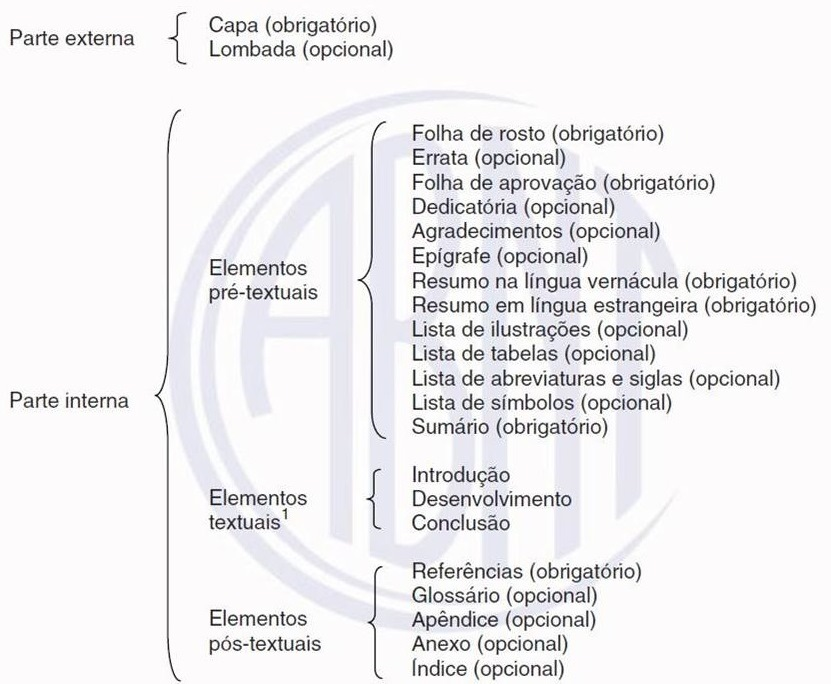
\includegraphics[scale=0.5]{USPSC-img/USPSC-EstruturaTrabAcad.jpg}
	\end{center}
	\legend{Fonte: \citeonline{nbr14724}}
\end{figure}

A vers\~ao v.3.1 do Pacote USPSC, por \textit{default}, \'e instalado em uma pasta denominada USPSC-v3.1 com a seguinte distribui\c{c}\~ao dos arquivos utilizados para gerar o documento em formato PDF, mediante a compila\c{c}\~ao utilizando um dos editores \LaTeX\ :


\begin{alineas}	
	\item \verb+ ...\USPSC-v3.1\ + contendo:	
		\begin{alineas}
			\item arquivo principal do tutorial: USPSC-tutorial.tex;
			\item arquivos principais do modelo para teses e disserta\c{c}\~oes:
				\begin{subalineas}
					\item USPSC-modelo.tex;
					\item USPSC-modelo-EESC.tex;
					\item USPSC-modelo-IAU.tex;
					\item USPSC-modelo-ICMCe.tex (idioma do texto em ingl\^es);
					\item USPSC-modelo-ICMCp.tex (idioma do texto em portugu\^es);
					\item USPSC-modelo-IFSCe.tex (idioma do texto em ingl\^es);
					\item USPSC-modelo-IFSCp.tex (idioma do texto em portugu\^es);
					\item USPSC-modelo-IQSC.tex;
				\end{subalineas}
			\item arquivos principais do modelo para TCC: 
			\begin{subalineas}
				\item USPSC-TCC-modelo.tex;
				\item USPSC-TCC-modelo-EESC.tex;
				\item USPSC-TCC-modelo-ICMCe.tex (idioma do texto em ingl\^es);
				\item USPSC-TCC-modelo-ICMCp.tex (idioma do texto em portugu\^es);
				\item USPSC-TCC-modelo-IQSC.tex;
			\end{subalineas}
			\item arquivo que relaciona os arquivos pr\'e-textuais dos programas de P\'os-Gradua\c{c}\~ao e TCCs das Unidades: USPSC-unidades.tex;
			\item arquivos pr\'e-textuais: USPSC-pre-textual-UUUU.tex e USPSC-TCC-pre-textual-UUUU.tex;
			\item pastas especificadas nos itens abaixo;
	   	\end{alineas}
	   	
	\item \verb+ ...\USPSC-v3.1\USPSC-bib\ + com o arquivo de dados das cita\c{c}\~oes e refer\^encias utilizadas: 
		\begin{alineas}	
			\item USPSC-modelo-references.bib;
		\end{alineas} 
		
	\item \verb+ ...\USPSC-v3.1\USPSC-classe\ + com os arquivos da classe USPSC, incluindo os referentes \`a compatibiliza\c{c}\~ao com a ABNT NBR 6023:2018:
		\begin{alineas}
			\item USPSC.cls;
			\item USPSC1.cls; 
			\item arquivo ABNT6023-2018.sty, para tirar <> da URL, chamado mediante o comando  \verb+ \usepackage{USPSC-classe/ABNT6023-2018}+;
			\item as demais compatibiliza\c{c}\~oes est\~ao nos arquivos abntex2-alf-USPSC.bst, abntex2-alfeng-USPSC.bst, abntex2-num-USPSC.bst e abntex2-numeng-USPSC.bst, chamados atrav\'es do comando \newline \verb+\bibliographystyle{USPSC-classe/abntex2-alf-USPSC} + ou \newline
			\verb+\bibliographystyle{USPSC-classe/abntex2-alfeng-USPSC} + ou \newline
			\verb+\bibliographystyle{USPSC-classe/abntex2-num-USPSC}+ ou \newline \verb+\bibliographystyle{USPSC-classe/abntex2-numeng-USPSC}+, dependendo se o Sistemas de chamada for autor-data ou num\'erico; 
		\end{alineas}	
	    
	\item \verb+ ...\USPSC-v3.1\USPSC-Tutorial\ + contendo:
		\begin{subalineas}
			\item USPSC-fichacatalograficaTutorial.tex;
			\item USPSC-ErrataTutorial.tex;
			\item USPSC-DedicatoriaTutorial.tex;
			\item USPSC-AgradecimentosTutorial.tex;
			\item USPSC-EpigrafeTutorial.tex;
			\item USPSC-ResumoTutorial.tex;
			\item USPSC-AbstractTutorial.tex;
			\item USPSC-AbreviaturasSiglasTutorial.tex;
			\item USPSC-SimbolosTutorial.tex;
			\item USPSC-Cap1-IntroducaoTutorial.tex;
			\item USPSC-Cap2-DesenvolvimentoTutorial;
			\item USPSC-Cap3-CitacoesTutorial.tex;
			\item USPSC-Cap4-ReferenciasTutorial.tex;
			\item USPSC-Cap5-ConclusaoTutorial.tex;
			\item USPSC-ApendicesTutorial.tex;
			\item USPSC-AnexosTutorial.tex;
			\item USPSC-IndicesRemissivosTutorial.tex.
		\end{subalineas}
	
	\item \verb+ ...\USPSC-v3.1\USPSC-TA-PreTextual\ + com os arquivos relativos aos elementos pr\'e-textuais de trabalhos acad\^emicos:
		\begin{alineas}
				\item USPSC-CapaICMC.tex;
				\item USPSC-fichacatalografica.tex;
				\item USPSC-fichacatalografica.pdf;
				\item USPSC-folhadeaprovacao.tex;
				\item USPSC-folhadeaprovacao.pdf;
				\item USPSC-Errata.tex;
				\item USPSC-Dedicatoria.tex;
				\item USPSC-Agradecimentos.tex;
				\item USPSC-Epigrafe.tex;
				\item USPSC-Resumo.tex;
				\item USPSC-Abstract.tex;
				\item USPSC-AbreviaturasSiglas.tex
				\item USPSC-Simbolos.tex 
				\item USPSC-PaginaEmBranco.pdf
			\end{alineas}
			
	\item \verb+ ...\USPSC-v3.1\USPSC-TA-Textual\ + contendo os arquivos relativos aos elementos textuais de trabalhos acad\^emicos:
		\begin{alineas}
			\item USPSC-Cap1-Introducao.tex;
			\item USPSC-Cap2-Desenvolvimento.tex;
			\item USPSC-Cap3-Conclusao.tex;
		\end{alineas}
		
	\item \verb+ ...\USPSC-v3.1\USPSC-TA-PosTextual\ + para os arquivos relativos aos elementos p\'os-textuais de trabalhos acad\^emicos:	
		\begin{alineas}
			\item USPSC-Apendices.tex;
			\item USPSC-Anexos.tex;
			\item USPSC-IndicesRemissivos.tex;
		\end{alineas}
	
	\item \verb+ ...\USPSC-v3.1\USPSC-img\ + contendo os arquivos de imagens e os PDFs relacionados no texto dos modelos: 
		\begin{alineas}	
			\item USPSC-AcentuacaoLaTeX.png;
			\item CapaICMC.jpg;
			\item USPSC-EstruturaTrabAcad.jpg;
			\item USPSC-LetrasGregas.png;
			\item USPSC-modelo-img-grafico.pdf;
			\item USPSC-modelo-img-marca.pdf;
			\item USPSC-SimbolosUteis.png;
		\end{alineas}	
	
	\item \verb+ ...\USPSC-v3.1\USPSC-Siglas\ + traz os arquivos que relacionam as siglas das Unidades e as definidas para os cursos de gradua\c{c}\~ao e programas de p\'os-gradua\c{c}\~ao, que n\~ao necessariamente s\~ao as oficiais utilizadas pela Universidade: 
		\begin{alineas}	
			\item USPSC-Siglas estabelecidas para os Programas de P\'os-Gradua\c{c}\~ao por Unidade.xlsx;
			\item USPSC-TCC-Siglas estabelecidas para as Gradua\c{c}\~oes por Unidade.xlsx;
		\end{alineas}
		
	\item \verb+ ...\USPSC-v3.1\USPSC-Sobre\ + cont\'em arquivos sobre cada vers\~ao do Pacote USPSC.

\end{alineas}	 

		
Para tese ou disserta\c{c}\~ao dever\'a ser utilizado o arquivo USPSC-modelo.tex, onde o autor dever\'a indicar a sigla da Unidade e a sigla do programa de p\'os-gradua\c{c}\~ao que est\'a vinculado, a exemplo dos comandos abaixo:
		
			\begin{verbatim}
				\siglaunidade{IQSC}
				\programa{MQOB}
			\end{verbatim}
			
Para o \textbf{Modelo para teses e disserta\c{c}\~oes em \LaTeX\ utilizando o Pacote USPSC} est\~ao definidos os seguintes arquivos pr\'e-textuais:
			
			\begin{alineas}	 
				\item USPSC-pre-textual-EESC.tex;
				\item USPSC-pre-textual-IAU.tex;
				\item USPSC-pre-textual-ICMC.tex;
				\item USPSC-pre-textual-IFSC.tex;
				\item USPSC-pre-textual-IQSC.tex.
			\end{alineas}
			
Para TCC dever\'a ser utilizado o arquivo USPSC-TCC-modelo.tex, onde o autor dever\'a indicar a \textbf{'sigla da Unidade'} + \textbf{'-TCC'} (Exemplo: EESC-TCC) e a sigla do curso de gradua\c{c}\~ao que est\'a vinculado, a exemplo dos comandos abaixo:
			
			\begin{verbatim}
			\siglaunidade{EESC-TCC}
			\programa{EAMB}
			\end{verbatim}
			
Atualmente est\~ao dispon\'{\i}veis os dados pr\'e-textuais para a EESC, ICMC e IQSC:
			
			\begin{alineas}	 
				\item USPSC-TCC-pre-textual-EESC.tex;
				\item USPSC-TCC-pre-textual-ICMC.tex;
				\item USPSC-TCC-pre-textual-IQSC.tex.
			\end{alineas}
			
Ser\~ao inclu\'{\i}dos os demais arquivos quando as demais Unidades do Campus USP de S\~ao Carlos estabelecerem seus padr\~oes. 
			
Para utilizar corretamente os dados pr\'e-textuais, \'e necess\'ario consultar as siglas estabelecidas para os cursos de gradua\c{c}\~ao e para os programas de p\'os-gradua\c{c}\~ao da Unidade de v\'{\i}nculo nos quadros dos \textbf{AP\^ENDICES B-I} ou nas planilhas \textbf{USPSC-TCC-Siglas estabelecidas para as Gradua\c{c}\~oes por Unidade.xlsx} e \textbf{USPSC-Siglas estabelecidas para os programas de p\'os-gradua\c{c}\~ao por Unidade.xlsx}. 

Os arquivos com dados pre-textuais est\~ao nominados como USPSC-pre-textual-UUUU.tex ou USPSC-TCC-pre-textual-UUUU.tex, onde UUUU \'e a sigla da Unidade. Inicialmente est\~ao disponibilizados apenas os pr\'e-textuais das Unidades do Campus USP de S\~ao Carlos.
			
Foram definidos os arquivos USPSC-pre-textual-OUTRO.tex e USPSC-TCC-pre-textual-OUTRO.tex que ser\~ao executados quando uma das siglas for diferente das explicitadas para as Unidades e/ou para os cursos de gradua\c{c}\~ao e/ou para os programas de P\'os-Gradua\c{c}\~ao. O pre\^ambulo ser\'a incompleto e apresentando "..." no final, evidenciando que o autor dever\'a rever as siglas utilizadas.

Atrav\'es do comando \verb+ %% USPSC-unidades.tex
% Camando para defini\c{c}\~ao do programa de P\'os-Gradua\c{c}\~ao, Especialidade do T\'{\i}tulo e Institui\c{c}\~ao
\newcommand{\siglaunidade}[1]{


% EESC-TCC ==========================================================================
    \ifthenelse{\equal{#1}{EESC-TCC}}{
     			%% USPSC-TCC-pre-textual-EESC.tex
%% Camandos para defini��o do tipo de documento (tese ou disserta��o), �rea de concentra��o, op��o, pre�mbulo, titula��o 
%% referentes aos Programas de P�s-Gradua��o
\instituicao{Faculdade de Educa\c{c}\~ao, Universidade Tecnol\'ogica Federal do Paran\'a - Campus Londrina}
\unidade{FACULDADE DE EDUCA\c{C}\~AO}
\unidademin{Faculdade de Educa\c{c}\~ao}
\universidademin{Universidade Tecnol\'ogica Federal do Paran\'a - Campus Londrina}
% A EESC n�o inclui a nota "Vers�o original", portanto o comando abaixo n�o tem a mensagem entre {}
\notafolharosto{ }
%Para a vers�o corrigida tire a % do comando/declara��o abaixo e inclua uma % antes do comando acima
%\notafolharosto{VERS\~AO CORRIGIDA}
% ---
% dados complementares para CAPA e FOLHA DE ROSTO
% ---
\universidade{UNIVERSIDADE TECNOL\'OGICA FEDERAL DO PARAN\'A - Campus Londrina}
\titulo{Caracteriza\c{c}\~ao do Projeto Workshop Aficionados por Software e Hardware (WASH) - Hist\'oria, M\'etodos e Resultados}
\titleabstract{Characterization of the Hardware and Software for Geeks Program }
\tituloresumo{Caracteriza\c{c}\~ao do Projeto Workshop Aficionados por Software e Hardware (WASH) - Hist\'oria, M\'etodos e Resultados}
\autor{Elaine da Silva Tozzi}
\autorficha{Tozzi, Elaine da Silva}
\autorabr{Tozzi, E.S.}

\cutter{S856m}
% Para gerar a ficha catalogr�fica sem o C�digo Cutter, basta 
% incluir uma % na linha acima e tirar a % da linha abaixo
%\cutter{ }

\local{Londrina}
\data{2022}
% Quando for Orientador, basta incluir uma % antes do comando abaixo
\renewcommand{\orientadorname}{Orientadora:}
% Quando for Coorientadora, basta tirar a % do comando abaixo
%\newcommand{\coorientadorname}{Coorientador:}
\orientador{Prof(a). Dr(a). Paulo S\'ergio Camargo}
%\orientadorcorpoficha{orientador(a) Paulo S\'ergio Camargo}
%\orientadorficha{Camargo, Paulo S\'ergio}
%Se houver co-orientador, inclua % antes das duas linhas (antes dos comandos \orientadorcorpoficha e \orientadorficha) 
%          e tire a % antes dos 3 comandos abaixo
\coorientador{Prof(a). Dr(a). @[coorientador]@}
\orientadorcorpoficha{orientador(a) Paulo S\'ergio Camargo}
\orientadorficha{Camargo, Paulo S\'ergio}

\notaautorizacao{AUTORIZO A REPRODU\c{C}\~AO E DIVULGA\c{C}\~AO TOTAL OU PARCIAL DESTE TRABALHO, POR QUALQUER MEIO CONVENCIONAL OU ELETR\^ONICO PARA FINS DE ESTUDO E PESQUISA, DESDE QUE CITADA A FONTE.}
\notabib{~  ~}

\newcommand{\programa}[1]{


% EAMB ==========================================================================
\ifthenelse{\equal{#1}{EAMB}}{
    \tipotrabalho{Monografia (Trabalho de Conclus\~ao de Curso)}
    \tipotrabalhoabs{Monograph (Conclusion Course Paper)}
    %\area{Nome da �rea}
	%\opcao{Nome da Op��o}
    % O preambulo deve conter o tipo do trabalho, o objetivo, 
	% o nome da institui��o, a �rea de concentra��o e op��o quando houver
	\preambulo{Monografia apresentada ao Curso de P\'os-Gradua\c{c}\~ao, da Faculdade de Educa\c{c}\~ao da Universidade Tecnol\'ogica Federal do Paran\'a - Campus Londrina, como parte dos requisitos para obten\c{c}\~ao do t\'itulo de Mestre em Licenciatura.}
	\notaficha{Monografia (Gradua\c{c}\~ao em Engenharia Ambiental)}
    }{
% EAER ===========================================================================
\ifthenelse{\equal{#1}{EAER}}{
	\tipotrabalho{Monografia (Trabalho de Conclus\~ao de Curso)}
	\tipotrabalhoabs{Monograph (Conclusion Course Paper)}
	%\area{Nome da �rea}
	%\opcao{Nome da Op��o}
	% O preambulo deve conter o tipo do trabalho, o objetivo, 
	% o nome da institui��o, a �rea de concentra��o e op��o quando houver
	\preambulo{Monografia apresentada ao Curso de P\'os-Gradua\c{c}\~ao, da Faculdade de Educa\c{c}\~ao da Universidade Tecnol\'ogica Federal do Paran\'a - Campus Londrina, como parte dos requisitos para obten\c{c}\~ao do t\'itulo de Mestre em Licenciatura.}
	\notaficha{Monografia (Gradua\c{c}\~ao em Engenharia Aeron\'autica)}
    }{
% ECIV =======================================================================
\ifthenelse{\equal{#1}{ECIV}}{
    \tipotrabalho{Monografia (Trabalho de Conclus\~ao de Curso)}
    \tipotrabalhoabs{Monograph (Conclusion Course Paper)}
    %\area{Nome da �rea}
    %\opcao{Nome da Op��o}
    % O preambulo deve conter o tipo do trabalho, o objetivo, 
	% o nome da institui��o, a �rea de concentra��o e op��o quando houver
	\preambulo{Monografia apresentada ao Curso de P\'os-Gradua\c{c}\~ao, da Faculdade de Educa\c{c}\~ao da Universidade Tecnol\'ogica Federal do Paran\'a - Campus Londrina, como parte dos requisitos para obten\c{c}\~ao do t\'itulo de Mestre em Licenciatura.}
	\notaficha{Monografia (Gradua\c{c}\~ao em Engenharia Civil)}
    }{
% ECOM ===========================================================================
\ifthenelse{\equal{#1}{ECOM}}{
	\tipotrabalho{Monografia (Trabalho de Conclus\~ao de Curso)}
	\tipotrabalhoabs{Monograph (Conclusion Course Paper)}
	%\area{Nome da �rea}
	%\opcao{Nome da Op��o}
	% O preambulo deve conter o tipo do trabalho, o objetivo, 
	% o nome da institui��o, a �rea de concentra��o e op��o quando houver
	\preambulo{Monografia apresentada ao Curso de P\'os-Gradua\c{c}\~ao}\~ao, da Faculdade de Educa\c{c}\~ao e Faculdade de Educa\c{c}\~ao}\~ao da Universidade Tecnol\'ogica Federal do Paran\'a - Campus Londrina, como parte dos requisitos para obten\c{c}\~ao do t\'itulo de Mestre em LicenciaturaMestre em Licenciatura}\~ao.}
	\notaficha{Monografia (Gradua\c{c}\~ao em Engenharia de Computa\c{c}\~ao)}
    }{
% EELT ==========================================================================
\ifthenelse{\equal{#1}{EELT}}{
    \tipotrabalho{Monografia (Trabalho de Conclus\~ao de Curso)}
    \tipotrabalhoabs{Monograph (Conclusion Course Paper)}
	%\area{Nome da �rea}
    %\opcao{Nome da Op��o}
    % O preambulo deve conter o tipo do trabalho, o objetivo, 
    % o nome da institui��o, a �rea de concentra��o e op��o quando houver
    \preambulo{Monografia apresentada ao Curso de P\'os-Gradua\c{c}\~ao, da Faculdade de Educa\c{c}\~ao da Universidade Tecnol\'ogica Federal do Paran\'a - Campus Londrina, como parte dos requisitos para obten\c{c}\~ao do t\'itulo de Mestre em Licenciatura.}
    \notaficha{Monografia (Gradua\c{c}\~ao em Engenharia El\'etrica com \^Enfase em Eletr\^onica)}
    }{
% EELS ===========================================================================
\ifthenelse{\equal{#1}{EELS}}{
	\tipotrabalho{Monografia (Trabalho de Conclus\~ao de Curso)}
	\tipotrabalhoabs{Monograph (Conclusion Course Paper)}
	%\area{Nome da �rea}
	%\opcao{Nome da Op��o}
	% O preambulo deve conter o tipo do trabalho, o objetivo, 
	% o nome da institui��o, a �rea de concentra��o e op��o quando houver
	\preambulo{Monografia apresentada ao Curso de P\'os-Gradua\c{c}\~ao}\~ao, da Faculdade de Educa\c{c}\~ao da Universidade Tecnol\'ogica Federal do Paran\'a - Campus Londrina, como parte dos requisitos para obten\c{c}\~ao do t\'itulo de Mestre em Licenciatura.}
	\notaficha{Monografia (Gradua\c{c}\~ao em Engenharia El\'etrica com \^Enfase Sistemas de Energia e Automa\c{c}\~ao)}
    }{			
% EMAT ==========================================================================
\ifthenelse{\equal{#1}{EMAT}}{
    \tipotrabalho{Monografia (Trabalho de Conclus\~ao de Curso)}
    \tipotrabalhoabs{Monograph (Conclusion Course Paper)}
    %\area{Nome da �rea}
    %\opcao{Nome da Op��o}
    % O preambulo deve conter o tipo do trabalho, o objetivo, 
    % o nome da institui��o, a �rea de concentra��o e op��o quando houver
    \preambulo{Monografia apresentada ao Curso de P\'os-Gradua\c{c}\~ao, da Faculdade de Educa\c{c}\~ao da Universidade Tecnol\'ogica Federal do Paran\'a - Campus Londrina, como parte dos requisitos para obten\c{c}\~ao do t\'itulo de Mestre em Licenciatura.}
    \notaficha{Monografia (Gradua\c{c}\~ao em Engenharia de Materiais e Manufatura)}
    }{
% EMEC ===========================================================================
\ifthenelse{\equal{#1}{EMEC}}{
	\tipotrabalho{Monografia (Trabalho de Conclus\~ao de Curso)}
	\tipotrabalhoabs{Monograph (Conclusion Course Paper)}
	%\area{Nome da �rea}
	%\opcao{Nome da Op��o}
	% O preambulo deve conter o tipo do trabalho, o objetivo, 
	% o nome da institui��o, a �rea de concentra��o e op��o quando houver
	\preambulo{Monografia apresentada ao Curso de P\'os-Gradua\c{c}\~ao, da Faculdade de Educa\c{c}\~ao da Universidade Tecnol\'ogica Federal do Paran\'a - Campus Londrina, como parte dos requisitos para obten\c{c}\~ao do t\'itulo de Mestre em Licenciatura.}
	\notaficha{Monografia (Gradua\c{c}\~ao em Engenharia Mec\^anica)}
    }{			
% EMET ===========================================================================
\ifthenelse{\equal{#1}{EMET}}{
    \tipotrabalho{Monografia (Trabalho de Conclus\~ao de Curso)}
    \tipotrabalhoabs{Monograph (Conclusion Course Paper)}
    %\area{Nome da �rea}
    %\opcao{Nome da Op��o}
    % O preambulo deve conter o tipo do trabalho, o objetivo, 
    % o nome da institui��o, a �rea de concentra��o e op��o quando houver
    \preambulo{Monografia apresentada ao Curso de P\'os-Gradua\c{c}\~ao, da Faculdade de Educa\c{c}\~ao da Universidade Tecnol\'ogica Federal do Paran\'a - Campus Londrina, como parte dos requisitos para obten\c{c}\~ao do t\'itulo de Mestre em Licenciatura.}
    \notaficha{Monografia (Gradua\c{c}\~ao em Engenharia Mecatr\^onica)}
    }{		
% EPRO ===========================================================================
\ifthenelse{\equal{#1}{EPRO}}{
	\tipotrabalho{Monografia (Trabalho de Conclus\~ao de Curso)}
	\tipotrabalhoabs{Monograph (Conclusion Course Paper)}
	%\area{Nome da �rea}
	%\opcao{Nome da Op��o}
	% O preambulo deve conter o tipo do trabalho, o objetivo, 
	% o nome da institui��o, a �rea de concentra��o e op��o quando houver
	\preambulo{Monografia apresentada ao Curso de P\'os-Gradua\c{c}\~ao}\~ao, da Faculdade de Educa\c{c}\~ao da Universidade Tecnol\'ogica Federal do Paran\'a - Campus Londrina, como parte dos requisitos para obten\c{c}\~ao do t\'itulo de Mestre em LicenciaturaMestre em Licenciatura}\~ao.}
	\notaficha{Monografia (Gradua\c{c}\~ao em Engenharia de Produ\c{c}\~a)}
}{		         	
% Outros
	\tipotrabalho{Monografia (Trabalho de Conclus\~ao de Curso)}
	\tipotrabalhoabs{Monograph (Conclusion Course Paper)}
	%\area{Nome da �rea}
	%\opcao{Nome da Op��o}
	% O preambulo deve conter o tipo do trabalho, o objetivo, 
	% o nome da institui��o, a �rea de concentra��o e op��o quando houver
	\preambulo{Monografia apresentada ao Curso de P\'os-Gradua\c{c}\~ao?), da Faculdade de Educa\c{c}\~ao da Universidade Tecnol\'ogica Federal do Paran\'a - Campus Londrina, como parte dos requisitos para obten\c{c}\~ao do t\'itulo de Mestre em Licenciatura?).}
	\notaficha{Monografia (Gradua\c{c}\~ao em Engenharia (?))}		
        }}}}}}}}}}}
        				
% ---
    }{
% EESC ==========================================================================
	\ifthenelse{\equal{#1}{EESC}}{
	%% USPSC-pre-textual-EESC.tex
%% Camandos para defini��o do tipo de documento (tese ou disserta��o), �rea de concentra��o, op��o, pre�mbulo, titula��o 
%% referentes aos Programas de P�s-Gradua��o
\instituicao{Faculdade de Educa\c{c}\~ao, Universidade Tecnol\'ogica Federal do Paran\'a - Campus Londrina}
\unidade{FACULDADE DE EDUCA\c{C}\~AO}
\unidademin{Faculdade de Educa\c{c}\~ao}
\universidademin{Universidade Tecnol\'ogica Federal do Paran\'a - Campus Londrina}

% A EESC n�o inclui a nota "Vers�o original", portanto o comando abaixo n�o tem a mensagem entre {}
\notafolharosto{ }
%Para a vers�o corrigida tire a % do comando/declara��o abaixo e inclua uma % antes do comando acima
%\notafolharosto{VERS\~AO CORRIGIDA}
% ---
% dados complementares para CAPA e FOLHA DE ROSTO
% ---
\universidade{UNIVERSIDADE TECNOL\'OGICA FEDERAL DO PARAN\'A - Campus Londrina}
\titulo{Caracteriza\c{c}\~ao e modelagem do sistema heter\'arquico de aprendizagem do WASH}
\titleabstract{Characterization of the Hardware and Software for Geeks Program }
\tituloresumo{Caracteriza\c{c}\~ao e modelagem do sistema heter\'arquico de aprendizagem do WASH}
\autor{Elaine da Silva Tozzi}
\autorficha{Tozzi, Elaine da Silva}
\autorabr{Tozzi, E.S.}

\cutter{S856m}
% Para gerar a ficha catalogr�fica sem o C�digo Cutter, basta 
% incluir uma % na linha acima e tirar a % da linha abaixo
%\cutter{ }

\local{Londrina}
\data{2022}
% Quando for Orientador, basta incluir uma % antes do comando abaixo
\renewcommand{\orientadorname}{Orientadora:}
% Quando for Coorientadora, basta tirar a % utilizar o comando abaixo
%\newcommand{\coorientadorname}{Coorientador:}
\orientador{Prof(a). Dr(a). Paulo S\'ergio Camargo e Victor Pellegrini Mammana}
\orientadorcorpoficha{orientador(a) Paulo S\'ergio Camargo e Victor Pellegrini Mammana}
\orientadorficha{Camargo, Paulo S\'ergio e Mammana, Victor Pellegrini}
%Se houver co-orientador, inclua % antes das duas linhas (antes dos comandos \orientadorcorpoficha e \orientadorficha) 
%          e tire a % antes dos 3 comandos abaixo
%\coorientador{Prof(a). Dr(a). @[coorientador]@}
%\orientadorcorpoficha{orientador(a) Paulo S\'ergio Camargo e Victor Pellegrini Mammana}
%\orientadorficha{Camargo, Paulo S\'ergio e Mammana, Victor Pellegrini}

\notaautorizacao{AUTORIZO A REPRODU\c{C}\~AO E DIVULGA\c{C}\~AO TOTAL OU PARCIAL DESTE TRABALHO, POR QUALQUER MEIO CONVENCIONAL OU ELETR\^ONICO PARA FINS DE ESTUDO E PESQUISA, DESDE QUE CITADA A FONTE.}
\notabib{~  ~}

\newcommand{\programa}[1]{

% DCEA ==========================================================================
\ifthenelse{\equal{#1}{DCEA}}{
    \tipotrabalho{Tese (Doutorado)}
    \tipotrabalhoabs{Thesis (Doctor)}
    \area{Ci\^encias da Engenharia Ambiental}
	%\opcao{Nome da Op��o}
    % O preambulo deve conter o tipo do trabalho, o objetivo, 
	% o nome da institui��o, a �rea de concentra��o e op��o quando houver
	\preambulo{Tese apresentada \`a Faculdade de Educa\c{c}\~ao da Universidade Tecnol\'ogica Federal do Paran\'a - Campus Londrina, para obten\c{c}\~ao do t\'itulo de Mestre em LicenciaturaMestre em Ci\^encias - Programa de P\'os-Gradua\c{c}\~ao da UTFPR.}
	\notaficha{Tese (Doutorado) - Programa de P\'os-Gradua\c{c}\~ao e \'Area de Concentra\c{c}\~ao em Ci\^encias da Engenharia Ambiental}
    }{
% MCEA ===========================================================================
\ifthenelse{\equal{#1}{MCEA}}{
	\tipotrabalho{Disserta\c{c}\~ao (Mestrado)}
	\tipotrabalhoabs{Dissertation (Master)}
	\area{Ci\^encias da Engenharia Ambiental}
	%\opcao{Nome da Op��o}
	% O preambulo deve conter o tipo do trabalho, o objetivo, 
	% o nome da institui��o, a �rea de concentra��o e op��o quando houver
	\preambulo{Disserta\c{c}\~ao apresentada \`a Faculdade de Educa\c{c}\~ao da Universidade Tecnol\'ogica Federal do Paran\'a - Campus Londrina, para obten\c{c}\~ao do t\'itulo de Mestre em LicenciaturaMestre em Ci\^encias - Programa de P\'os-Gradua\c{c}\~ao da UTFPR.}
	\notaficha{Disserta\c{c}\~ao (Mestrado) - Programa de P\'os-Gradua\c{c}\~ao e \'Area de Concentra\c{c}\~ao em Ci\^encias da Engenharia Ambiental}
        }{
% DEE =======================================================================
\ifthenelse{\equal{#1}{DEE}}{
    \tipotrabalho{Tese (Doutorado)}
    \tipotrabalhoabs{Thesis (Doctor)}
    \area{Estruturas}
	%\opcao{Nome da Op��o}
    % O preambulo deve conter o tipo do trabalho, o objetivo, 
	% o nome da institui��o, a �rea de concentra��o e op��o quando houver
	\preambulo{Tese apresentada \`a Faculdade de Educa\c{c}\~ao da Universidade Tecnol\'ogica Federal do Paran\'a - Campus Londrina, para obten\c{c}\~ao do t\'itulo de Mestre em LicenciaturaMestre em Ci\^encias - Programa de P\'os-Gradua\c{c}\~ao da UTFPR.}
	\notaficha{Tese (Doutorado) - Programa de P\'os-Gradua\c{c}\~ao da UTFPR}
    }{
% MEE ===========================================================================
\ifthenelse{\equal{#1}{MEE}}{
	\tipotrabalho{Disserta\c{c}\~ao (Mestrado)}
	\tipotrabalhoabs{Dissertation (Master)}
	\area{Estruturas}
	%\opcao{Nome da Op��o}
	% O preambulo deve conter o tipo do trabalho, o objetivo, 
	% o nome da institui��o, a �rea de concentra��o e op��o quando houver
	\preambulo{Disserta\c{c}\~ao apresentada \`a Faculdade de Educa\c{c}\~ao da Universidade Tecnol\'ogica Federal do Paran\'a - Campus Londrina, para obten\c{c}\~ao do t\'itulo de Mestre em LicenciaturaMestre em Ci\^encias - Programa de P\'os-Gradua\c{c}\~ao da UTFPR.}
	\notaficha{Disserta\c{c}\~ao (Mestrado) - Programa de P\'os-Gradua\c{c}\~ao da UTFPR}
    }{
% DEPP ==========================================================================
\ifthenelse{\equal{#1}{DEPP}}{
    \tipotrabalho{Tese (Doutorado)}
    \tipotrabalhoabs{Thesis (Doctor)}
    \area{Processos e Gest\~ao de Opera\c{c}\~oes}
	%\opcao{Nome da Op��o}
    % O preambulo deve conter o tipo do trabalho, o objetivo, 
	% o nome da institui��o, a �rea de concentra��o e op��o quando houver
	\preambulo{Tese apresentada \`a Faculdade de Educa\c{c}\~ao da Universidade Tecnol\'ogica Federal do Paran\'a - Campus Londrina, para obten\c{c}\~ao do t\'itulo de Mestre em LicenciaturaMestre em Ci\^encias - Programa de P\'os-Gradua\c{c}\~ao da UTFPR}\~ao.}
	\notaficha{Tese (Doutorado) - Programa de P\'os-Gradua\c{c}\~ao da UTFPR}
    }{
% MEPP ===========================================================================
\ifthenelse{\equal{#1}{MEPP}}{
	\tipotrabalho{Disserta\c{c}\~ao (Mestrado)}
	\tipotrabalhoabs{Dissertation (Master)}
	\area{Processos e Gest\~ao de Opera\c{c}\~oes}
	%\opcao{Nome da Op��o}
	% O preambulo deve conter o tipo do trabalho, o objetivo, 
	% o nome da institui��o, a �rea de concentra��o e op��o quando houver
	\preambulo{Disserta\c{c}\~ao apresentada \`a Faculdade de Educa\c{c}\~ao da Universidade Tecnol\'ogica Federal do Paran\'a - Campus Londrina, para obten\c{c}\~ao do t\'itulo de Mestre em LicenciaturaMestre em Ci\^encias - Programa de P\'os-Gradua\c{c}\~ao da UTFPR}\~ao.}
	\notaficha{Disserta\c{c}\~ao (Mestrado) - Programa de P\'os-Gradua\c{c}\~ao da UTFPR}
    }{			
% DEPE ==========================================================================
\ifthenelse{\equal{#1}{DEPE}}{
    \tipotrabalho{Tese (Doutorado)}
    \tipotrabalhoabs{Thesis (Doctor)}
    \area{Economia, Organiza\c{c}\~oes e Gest\~ao do Conhecimento}
	%\opcao{Nome da Op��o}
    % O preambulo deve conter o tipo do trabalho, o objetivo, 
	% o nome da institui��o, a �rea de concentra��o e op��o quando houver
	\preambulo{Tese apresentada \`a Faculdade de Educa\c{c}\~ao da Universidade Tecnol\'ogica Federal do Paran\'a - Campus Londrina, para obten\c{c}\~ao do t\'itulo de Mestre em LicenciaturaMestre em Ci\^encias - Programa de P\'os-Gradua\c{c}\~ao da UTFPR}\~ao.}
	\notaficha{Tese (Doutorado) - Programa de P\'os-Gradua\c{c}\~ao da UTFPR}\~ao em Economia, Organiza\c{c}\~oes e Gest\~ao do Conhecimento}
    }{
% MEPE ===========================================================================
\ifthenelse{\equal{#1}{MEPE}}{
	\tipotrabalho{Disserta\c{c}\~ao (Mestrado)}
	\tipotrabalhoabs{Dissertation (Master)}
	\area{Economia, Organiza\c{c}\~oes e Gest\~ao do Conhecimento}
	%\opcao{Nome da Op��o}
	% O preambulo deve conter o tipo do trabalho, o objetivo, 
	% o nome da institui��o, a �rea de concentra��o e op��o quando houver
	\preambulo{Disserta\c{c}\~ao apresentada \`a Faculdade de Educa\c{c}\~ao da Universidade Tecnol\'ogica Federal do Paran\'a - Campus Londrina, para obten\c{c}\~ao do t\'itulo de Mestre em LicenciaturaMestre em Ci\^encias - Programa de P\'os-Gradua\c{c}\~ao da UTFPR}\~ao.}
	\notaficha{Disserta\c{c}\~ao (Mestrado) - Programa de P\'os-Gradua\c{c}\~ao da UTFPR}\~ao em Economia, Organiza\c{c}\~oes e Gest\~ao do Conhecimento}
    }{			
% DETI ==========================================================================
\ifthenelse{\equal{#1}{DETI}}{
    \tipotrabalho{Tese (Doutorado)}
    \tipotrabalhoabs{Thesis (Doctor)}
    \area{Infraestrutura de Transportes}
	%\opcao{Nome da Op��o}
    % O preambulo deve conter o tipo do trabalho, o objetivo, 
	% o nome da institui��o, a �rea de concentra��o e op��o quando houver
	\preambulo{Tese apresentada \`a Faculdade de Educa\c{c}\~ao da Universidade Tecnol\'ogica Federal do Paran\'a - Campus Londrina, para obten\c{c}\~ao do t\'itulo de Mestre em LicenciaturaMestre em Ci\^encias - Programa de P\'os-Gradua\c{c}\~ao da UTFPR.}
	\notaficha{Tese (Doutorado) - Programa de P\'os-Gradua\c{c}\~ao da UTFPR}
    }{
% METI ===========================================================================
\ifthenelse{\equal{#1}{METI}}{
	\tipotrabalho{Disserta\c{c}\~ao (Mestrado)}
	\tipotrabalhoabs{Dissertation (Master)}
	\area{Infraestrutura de Transportes}
	%\opcao{Nome da Op��o}
	% O preambulo deve conter o tipo do trabalho, o objetivo, 
	% o nome da institui��o, a �rea de concentra��o e op��o quando houver
	\preambulo{Disserta\c{c}\~ao apresentada \`a Faculdade de Educa\c{c}\~ao da Universidade Tecnol\'ogica Federal do Paran\'a - Campus Londrina, para obten\c{c}\~ao do t\'itulo de Mestre em LicenciaturaMestre em Ci\^encias - Programa de P\'os-Gradua\c{c}\~ao da UTFPR.}
	\notaficha{Disserta\c{c}\~ao (Mestrado) - Programa de P\'os-Gradua\c{c}\~ao da UTFPR}
    }{	   			
% DETT ==========================================================================
\ifthenelse{\equal{#1}{DETT}}{
    \tipotrabalho{Tese (Doutorado)}
    \tipotrabalhoabs{Thesis (Doctor)}
    \area{Transportes}
	%\opcao{Nome da Op��o}
    % O preambulo deve conter o tipo do trabalho, o objetivo, 
	% o nome da institui��o, a �rea de concentra��o e op��o quando houver
	\preambulo{Tese apresentada \`a Faculdade de Educa\c{c}\~ao da Universidade Tecnol\'ogica Federal do Paran\'a - Campus Londrina, para obten\c{c}\~ao do t\'itulo de Mestre em LicenciaturaMestre em Ci\^encias - Programa de P\'os-Gradua\c{c}\~ao da UTFPR.}
	\notaficha{Tese (Doutorado) - Programa de P\'os-Gradua\c{c}\~ao da UTFPR}
    }{
% METT ===========================================================================
\ifthenelse{\equal{#1}{METT}}{
	\tipotrabalho{Disserta\c{c}\~ao (Mestrado)}
	\tipotrabalhoabs{Dissertation (Master)}
	\area{Transportes}
	%\opcao{Nome da Op��o}
	% O preambulo deve conter o tipo do trabalho, o objetivo, 
	% o nome da institui��o, a �rea de concentra��o e op��o quando houver
	\preambulo{Disserta\c{c}\~ao apresentada \`a Faculdade de Educa\c{c}\~ao da Universidade Tecnol\'ogica Federal do Paran\'a - Campus Londrina, para obten\c{c}\~ao do t\'itulo de Mestre em LicenciaturaMestre em Ci\^encias - Programa de P\'os-Gradua\c{c}\~ao da UTFPR.}
	\notaficha{Disserta\c{c}\~ao (Mestrado) - Programa de P\'os-Gradua\c{c}\~ao da UTFPR}
    }{	  				
% DETP ==========================================================================
\ifthenelse{\equal{#1}{DETP}}{
    \tipotrabalho{Tese (Doutorado)}
    \tipotrabalhoabs{Thesis (Doctor)}
    \area{Planejamento e Opera\c{c}\~ao de Sistemas de Transporte}
	%\opcao{Nome da Op��o}
    % O preambulo deve conter o tipo do trabalho, o objetivo, 
	% o nome da institui��o, a �rea de concentra��o e op��o quando houver
	\preambulo{Tese apresentada \`a Faculdade de Educa\c{c}\~ao da Universidade Tecnol\'ogica Federal do Paran\'a - Campus Londrina, para obten\c{c}\~ao do t\'itulo de Mestre em LicenciaturaMestre em Ci\^encias - Programa de P\'os-Gradua\c{c}\~ao da UTFPR.}
	\notaficha{Tese (Doutorado) - Programa de P\'os-Gradua\c{c}\~ao da UTFPR}
    }{
% METP ===========================================================================
\ifthenelse{\equal{#1}{METP}}{
	\tipotrabalho{Disserta\c{c}\~ao (Mestrado)}
	\tipotrabalhoabs{Dissertation (Master)}
	\area{Planejamento e Opera\c{c}\~ao de Sistemas de Transporte}
	%\opcao{Nome da Op��o}
	% O preambulo deve conter o tipo do trabalho, o objetivo, 
	% o nome da institui��o, a �rea de concentra��o e op��o quando houver
	\preambulo{Disserta\c{c}\~ao apresentada \`a Faculdade de Educa\c{c}\~ao da Universidade Tecnol\'ogica Federal do Paran\'a - Campus Londrina, para obten\c{c}\~ao do t\'itulo de Mestre em LicenciaturaMestre em Ci\^encias - Programa de P\'os-Gradua\c{c}\~ao da UTFPR.}
	\notaficha{Disserta\c{c}\~ao (Mestrado) - Programa de P\'os-Gradua\c{c}\~ao da UTFPR}
    }{	    
% DEEP ==========================================================================
\ifthenelse{\equal{#1}{DEEP}}{
    \tipotrabalho{Tese (Doutorado)}
    \tipotrabalhoabs{Thesis (Doctor)}
    \area{Processamento de Sinais e Instrumenta\c{c}\~ao}
	%\opcao{Nome da Op��o}
	% O preambulo deve conter o tipo do trabalho, o objetivo, 
	% o nome da institui��o, a �rea de concentra��o e op��o quando houver
	\preambulo{Tese apresentada \`a Faculdade de Educa\c{c}\~ao da Universidade Tecnol\'ogica Federal do Paran\'a - Campus Londrina, para obten\c{c}\~ao do t\'itulo de Mestre em LicenciaturaMestre em Ci\^encias - Programa de P\'os-Gradua\c{c}\~ao da UTFPR.}
	\notaficha{Tese (Doutorado) - Programa de P\'os-Gradua\c{c}\~ao da UTFPR}
    }{
% MEEP ===========================================================================
\ifthenelse{\equal{#1}{MEEP}}{
	\tipotrabalho{Disserta\c{c}\~ao (Mestrado)}
	\tipotrabalhoabs{Dissertation (Master)}
	\area{Processamento de Sinais e Instrumenta\c{c}\~ao}
	%\opcao{Nome da Op��o}
	% O preambulo deve conter o tipo do trabalho, o objetivo, 
	% o nome da institui��o, a �rea de concentra��o e op��o quando houver
	\preambulo{Disserta\c{c}\~ao apresentada \`a Faculdade de Educa\c{c}\~ao da Universidade Tecnol\'ogica Federal do Paran\'a - Campus Londrina, para obten\c{c}\~ao do t\'itulo de Mestre em LicenciaturaMestre em Ci\^encias - Programa de P\'os-Gradua\c{c}\~ao da UTFPR.}
	\notaficha{Disserta\c{c}\~ao (Mestrado) - Programa de P\'os-Gradua\c{c}\~ao da UTFPR}
    }{	  
% DEED ==========================================================================
\ifthenelse{\equal{#1}{DEED}}{
    \tipotrabalho{Tese (Doutorado)}
    \tipotrabalhoabs{Thesis (Doctor)}
    \area{Sistemas Din\^amicos}
	%\opcao{Nome da Op��o}
    % O preambulo deve conter o tipo do trabalho, o objetivo, 
	% o nome da institui��o, a �rea de concentra��o e op��o quando houver
	\preambulo{Tese apresentada \`a Faculdade de Educa\c{c}\~ao da Universidade Tecnol\'ogica Federal do Paran\'a - Campus Londrina, para obten\c{c}\~ao do t\'itulo de Mestre em LicenciaturaMestre em Ci\^encias - Programa de P\'os-Gradua\c{c}\~ao da UTFPR.}
	\notaficha{Tese (Doutorado) - Programa de P\'os-Gradua\c{c}\~ao da UTFPR}
    }{
% MEED ===========================================================================
\ifthenelse{\equal{#1}{MEED}}{
	\tipotrabalho{Disserta\c{c}\~ao (Mestrado)}
	\tipotrabalhoabs{Dissertation (Master)}
	\area{Sistemas Din\^amicos}
	%\opcao{Nome da Op��o}
	% O preambulo deve conter o tipo do trabalho, o objetivo, 
	% o nome da institui��o, a �rea de concentra��o e op��o quando houver
	\preambulo{Disserta\c{c}\~ao apresentada \`a Faculdade de Educa\c{c}\~ao da Universidade Tecnol\'ogica Federal do Paran\'a - Campus Londrina, para obten\c{c}\~ao do t\'itulo de Mestre em LicenciaturaMestre em Ci\^encias - Programa de P\'os-Gradua\c{c}\~ao da UTFPR.}
	\notaficha{Disserta\c{c}\~ao (Mestrado) - Programa de P\'os-Gradua\c{c}\~ao da UTFPR}
    }{	  
% DEEE ==========================================================================
\ifthenelse{\equal{#1}{DEEE}}{
    \tipotrabalho{Tese (Doutorado)}
    \tipotrabalhoabs{Thesis (Doctor)}
    \area{Sistemas El\'etricos de Pot\^encia}
	%\opcao{Nome da Op��o}
    % O preambulo deve conter o tipo do trabalho, o objetivo, 
	% o nome da institui��o, a �rea de concentra��o e op��o quando houver
	\preambulo{Tese apresentada \`a Faculdade de Educa\c{c}\~ao da Universidade Tecnol\'ogica Federal do Paran\'a - Campus Londrina, para obten\c{c}\~ao do t\'itulo de Mestre em LicenciaturaMestre em Ci\^encias - Programa de P\'os-Gradua\c{c}\~ao da UTFPR.}
	\notaficha{Tese (Doutorado) - Programa de P\'os-Gradua\c{c}\~ao da UTFPR}
    }{
% MEEE ===========================================================================
\ifthenelse{\equal{#1}{MEEE}}{
    \tipotrabalho{Disserta\c{c}\~ao (Mestrado)}
    \tipotrabalhoabs{Dissertation (Master)}
    \area{Sistemas El\'etricos de Pot\^encia}
	%\opcao{Nome da Op��o}
    % O preambulo deve conter o tipo do trabalho, o objetivo, 
	% o nome da institui��o, a �rea de concentra��o e op��o quando houver
	\preambulo{Disserta\c{c}\~ao apresentada \`a Faculdade de Educa\c{c}\~ao da Universidade Tecnol\'ogica Federal do Paran\'a - Campus Londrina, para obten\c{c}\~ao do t\'itulo de Mestre em LicenciaturaMestre em Ci\^encias - Programa de P\'os-Gradua\c{c}\~ao da UTFPR.}
	\notaficha{Disserta\c{c}\~ao (Mestrado) - Programa de P\'os-Gradua\c{c}\~ao da UTFPR}
    }{	  
% DEET ==========================================================================
\ifthenelse{\equal{#1}{DEET}}{
    \tipotrabalho{Tese (Doutorado)}
    \tipotrabalhoabs{Thesis (Doctor)}
    \area{Telecomunica\c{c}\~oes}
	%\opcao{Nome da Op��o}
    % O preambulo deve conter o tipo do trabalho, o objetivo, 
	% o nome da institui��o, a �rea de concentra��o e op��o quando houver
	\preambulo{Tese apresentada \`a Faculdade de Educa\c{c}\~ao da Universidade Tecnol\'ogica Federal do Paran\'a - Campus Londrina, para obten\c{c}\~ao do t\'itulo de Mestre em LicenciaturaMestre em Ci\^encias - Programa de P\'os-Gradua\c{c}\~ao da UTFPR.}
	\notaficha{Tese (Doutorado) - Programa de P\'os-Gradua\c{c}\~ao da UTFPR}
    }{
% MEET ===========================================================================
\ifthenelse{\equal{#1}{MEET}}{
	\tipotrabalho{Disserta\c{c}\~ao (Mestrado)}
	\area{Telecomunica\c{c}\~oes}
	%\opcao{Nome da Op��o}
	% O preambulo deve conter o tipo do trabalho, o objetivo, 
	% o nome da institui��o, a �rea de concentra��o e op��o quando houver
	\preambulo{Disserta\c{c}\~ao apresentada \`a Faculdade de Educa\c{c}\~ao da Universidade Tecnol\'ogica Federal do Paran\'a - Campus Londrina, para obten\c{c}\~ao do t\'itulo de Mestre em LicenciaturaMestre em Ci\^encias - Programa de P\'os-Gradua\c{c}\~ao da UTFPR.}
	\notaficha{Disserta\c{c}\~ao (Mestrado) - Programa de P\'os-Gradua\c{c}\~ao da UTFPR}
    }{	
% DEHS ==========================================================================
\ifthenelse{\equal{#1}{DEHS}}{
    \tipotrabalho{Tese (Doutorado)}
    \tipotrabalhoabs{Thesis (Doctor)}
    \area{Hidr\'aulica e Saneamento}
	%\opcao{Nome da Op��o}
    % O preambulo deve conter o tipo do trabalho, o objetivo, 
	% o nome da institui��o, a �rea de concentra��o e op��o quando houver
	\preambulo{Tese apresentada \`a Faculdade de Educa\c{c}\~ao da Universidade Tecnol\'ogica Federal do Paran\'a - Campus Londrina, para obten\c{c}\~ao do t\'itulo de Mestre em LicenciaturaMestre em Ci\^encias - Programa de P\'os-Gradua\c{c}\~ao da UTFPR.}
	\notaficha{Tese (Doutorado) - Programa de P\'os-Gradua\c{c}\~ao e \'Area de Concentra\c{c}\~ao em Engenharia Hidr\'aulica e Saneamento}
    }{
% MEHS ===========================================================================
\ifthenelse{\equal{#1}{MEHS}}{
	\tipotrabalho{Disserta\c{c}\~ao (Mestrado)}
	\tipotrabalhoabs{Dissertation (Master)}
	\area{Hidr\'aulica e Saneamento}
	%\opcao{Nome da Op��o}
	% O preambulo deve conter o tipo do trabalho, o objetivo, 
	% o nome da institui��o, a �rea de concentra��o e op��o quando houver
	\preambulo{Disserta\c{c}\~ao apresentada \`a Faculdade de Educa\c{c}\~ao da Universidade Tecnol\'ogica Federal do Paran\'a - Campus Londrina, para obten\c{c}\~ao do t\'itulo de Mestre em LicenciaturaMestre em Ci\^encias - Programa de P\'os-Gradua\c{c}\~ao da UTFPR.}
	\notaficha{Disserta\c{c}\~ao (Mestrado) - Programa de P\'os-Gradua\c{c}\~ao e \'Area de Concentra\c{c}\~ao em Engenharia Hidr\'aulica e Saneamento} 
    }{	
% DEMA ==========================================================================
\ifthenelse{\equal{#1}{DEMA}}{
    \tipotrabalho{Tese (Doutorado)}
    \tipotrabalhoabs{Thesis (Doctor)}
    \area{Aerona\'utica}
	%\opcao{Nome da Op��o}
    % O preambulo deve conter o tipo do trabalho, o objetivo, 
	% o nome da institui��o, a �rea de concentra��o e op��o quando houver
	\preambulo{Tese apresentada \`a Faculdade de Educa\c{c}\~ao da Universidade Tecnol\'ogica Federal do Paran\'a - Campus Londrina, para obten\c{c}\~ao do t\'itulo de Mestre em LicenciaturaMestre em Ci\^encias - Programa de P\'os-Gradua\c{c}\~ao da UTFPR.}
	\notaficha{Tese (Doutorado) - Programa de P\'os-Gradua\c{c}\~ao da UTFPR}
    }{
% MEMA ===========================================================================
\ifthenelse{\equal{#1}{MEMA}}{
	\tipotrabalho{Disserta\c{c}\~ao (Mestrado)}
	\tipotrabalhoabs{Dissertation (Master)}
	\area{Aerona\'utica}
	%\opcao{Nome da Op��o}
	% O preambulo deve conter o tipo do trabalho, o objetivo, 
	% o nome da institui��o, a �rea de concentra��o e op��o quando houver
	\preambulo{Disserta\c{c}\~ao apresentada \`a Faculdade de Educa\c{c}\~ao da Universidade Tecnol\'ogica Federal do Paran\'a - Campus Londrina, para obten\c{c}\~ao do t\'itulo de Mestre em LicenciaturaMestre em Ci\^encias - Programa de P\'os-Gradua\c{c}\~ao da UTFPR.}
	\notaficha{Disserta\c{c}\~ao (Mestrado) - Programa de P\'os-Gradua\c{c}\~ao da UTFPR}
    }{	
% DEMD ==========================================================================
\ifthenelse{\equal{#1}{DEMD}}{
    \tipotrabalho{Tese (Doutorado)}
    \tipotrabalhoabs{Thesis (Doctor)}
    \area{Din\^amica e Mecatr\^onica}
	%\opcao{Nome da Op��o}
    % O preambulo deve conter o tipo do trabalho, o objetivo, 
	% o nome da institui��o, a �rea de concentra��o e op��o quando houver
	\preambulo{Tese apresentada \`a Faculdade de Educa\c{c}\~ao da Universidade Tecnol\'ogica Federal do Paran\'a - Campus Londrina, para obten\c{c}\~ao do t\'itulo de Mestre em LicenciaturaMestre em Ci\^encias - Programa de P\'os-Gradua\c{c}\~ao da UTFPR.}
	\notaficha{Tese (Doutorado) - Programa de P\'os-Gradua\c{c}\~ao da UTFPR}
    }{
% MEMD ===========================================================================
\ifthenelse{\equal{#1}{MEMD}}{
	\tipotrabalho{Disserta\c{c}\~ao (Mestrado)}
	\tipotrabalhoabs{Dissertation (Master)}
	\area{Din\^amica e Mecatr\^onica}
	%\opcao{Nome da Op��o}
	% O preambulo deve conter o tipo do trabalho, o objetivo, 
	% o nome da institui��o, a �rea de concentra��o e op��o quando houver
	\preambulo{Disserta\c{c}\~ao apresentada \`a Faculdade de Educa\c{c}\~ao da Universidade Tecnol\'ogica Federal do Paran\'a - Campus Londrina, para obten\c{c}\~ao do t\'itulo de Mestre em LicenciaturaMestre em Ci\^encias - Programa de P\'os-Gradua\c{c}\~ao da UTFPR.}
	\notaficha{Disserta\c{c}\~ao (Mestrado) - Programa de P\'os-Gradua\c{c}\~ao da UTFPR}
    }{	
% DEMF ==========================================================================
\ifthenelse{\equal{#1}{DEMF}}{
    \tipotrabalho{Tese (Doutorado)}
    \tipotrabalhoabs{Thesis (Doctor)}
    \area{Projeto, Materiais e Manufatura}
	%\opcao{Nome da Op��o}
    % O preambulo deve conter o tipo do trabalho, o objetivo, 
	% o nome da institui��o, a �rea de concentra��o e op��o quando houver
	\preambulo{Tese apresentada \`a Faculdade de Educa\c{c}\~ao da Universidade Tecnol\'ogica Federal do Paran\'a - Campus Londrina, para obten\c{c}\~ao do t\'itulo de Mestre em LicenciaturaMestre em Ci\^encias - Programa de P\'os-Gradua\c{c}\~ao da UTFPR.}
	\notaficha{Tese (Doutorado) - Programa de P\'os-Gradua\c{c}\~ao da UTFPR}\~ao em Projeto, Materiais e Manufatura}
    }{
% MEMF ===========================================================================
\ifthenelse{\equal{#1}{MEMF}}{
	\tipotrabalho{Disserta\c{c}\~ao (Mestrado)}
	\tipotrabalhoabs{Dissertation (Master)}
	\area{Projeto, Materiais e Manufatura}
	%\opcao{Nome da Op��o}
	% O preambulo deve conter o tipo do trabalho, o objetivo, 
	% o nome da institui��o, a �rea de concentra��o e op��o quando houver
	\preambulo{Disserta\c{c}\~ao apresentada \`a Faculdade de Educa\c{c}\~ao da Universidade Tecnol\'ogica Federal do Paran\'a - Campus Londrina, para obten\c{c}\~ao do t\'itulo de Mestre em LicenciaturaMestre em Ci\^encias - Programa de P\'os-Gradua\c{c}\~ao da UTFPR.}
	\notaficha{Disserta\c{c}\~ao (Mestrado) - Programa de P\'os-Gradua\c{c}\~ao da UTFPR}\~ao em Projeto, Materiais e Manufatura}
    }{	
% DEMT ==========================================================================
\ifthenelse{\equal{#1}{DEMT}}{
    \tipotrabalho{Tese (Doutorado)}
    \tipotrabalhoabs{Thesis (Doctor)}
    \area{Termoci\^encias e Mec\^anica de Fluidos}
	%\opcao{Nome da Op��o}
    % O preambulo deve conter o tipo do trabalho, o objetivo, 
	% o nome da institui��o, a �rea de concentra��o e op��o quando houver
	\preambulo{Tese apresentada \`a Faculdade de Educa\c{c}\~ao da Universidade Tecnol\'ogica Federal do Paran\'a - Campus Londrina, para obten\c{c}\~ao do t\'itulo de Mestre em LicenciaturaMestre em Ci\^encias - Programa de P\'os-Gradua\c{c}\~ao da UTFPR.}
	\notaficha{Tese (Doutorado) - Programa de P\'os-Gradua\c{c}\~ao da UTFPR}
    }{
% MEMT ===========================================================================
\ifthenelse{\equal{#1}{MEMT}}{
	\tipotrabalho{Disserta\c{c}\~ao (Mestrado)}
	\tipotrabalhoabs{Dissertation (Master)}
	\area{Termoci\^encias e Mec\^anica de Fluidos}
	%\opcao{Nome da Op��o}
	% O preambulo deve conter o tipo do trabalho, o objetivo, 
	% o nome da institui��o, a �rea de concentra��o e op��o quando houver
	\preambulo{Disserta\c{c}\~ao apresentada \`a Faculdade de Educa\c{c}\~ao da Universidade Tecnol\'ogica Federal do Paran\'a - Campus Londrina, para obten\c{c}\~ao do t\'itulo de Mestre em LicenciaturaMestre em Ci\^encias - Programa de P\'os-Gradua\c{c}\~ao da UTFPR.}
	\notaficha{Disserta\c{c}\~ao (Mestrado) - Programa de P\'os-Gradua\c{c}\~ao da UTFPR}
    }{	
% DCEM ==========================================================================
\ifthenelse{\equal{#1}{DCEM}}{
    \tipotrabalho{Tese (Doutorado)}
    \tipotrabalhoabs{Thesis (Doctor)}
    \area{Caracteriza\c{c}\~ao, Desenvolvimento e Aplica\c{c}\~ao de Materiais}
	%\opcao{Nome da Op��o}
    % O preambulo deve conter o tipo do trabalho, o objetivo, 
	% o nome da institui��o, a �rea de concentra��o e op��o quando houver
	\preambulo{Tese apresentada \`a Faculdade de Educa\c{c}\~ao da Universidade Tecnol\'ogica Federal do Paran\'a - Campus Londrina, para obten\c{c}\~ao do t\'itulo de Mestre em LicenciaturaMestre em Ci\^encias - Programa de P\'os-Gradua\c{c}\~ao da UTFPR.}
	\notaficha{Tese (Doutorado) - Programa de P\'os-Gradua\c{c}\~ao da UTFPR}\~ao em Desenvolvimento, Caracteriza\c{c}\~ao e Aplica\c{c}\~ao de Materiais}
    }{
% MCEM ===========================================================================
\ifthenelse{\equal{#1}{MCEM}}{
	\tipotrabalho{Disserta\c{c}\~ao (Mestrado)}
	\tipotrabalhoabs{Dissertation (Master)}
	\area{Caracteriza\c{c}\~ao, Desenvolvimento e Aplica\c{c}\~ao de Materiais}
	%\opcao{Nome da Op��o}
	% O preambulo deve conter o tipo do trabalho, o objetivo, 
	% o nome da institui��o, a �rea de concentra��o e op��o quando houver
	\preambulo{Disserta\c{c}\~ao apresentada \`a Faculdade de Educa\c{c}\~ao da Universidade Tecnol\'ogica Federal do Paran\'a - Campus Londrina, para obten\c{c}\~ao do t\'itulo de Mestre em LicenciaturaMestre em Ci\^encias - Programa de P\'os-Gradua\c{c}\~ao da UTFPR.}
	\notaficha{Disserta\c{c}\~ao (Mestrado) - Programa de P\'os-Gradua\c{c}\~ao da UTFPR}\~ao em Desenvolvimento, Caracteriza\c{c}\~ao e Aplica\c{c}\~ao de Materiais}
    }{	
% DGEO ==========================================================================
\ifthenelse{\equal{#1}{DGEO}}{
    \tipotrabalho{Tese (Doutorado)}
    \tipotrabalhoabs{Thesis (Doctor)}
    \area{Geotecnia}
	%\opcao{Nome da Op��o}
    % O preambulo deve conter o tipo do trabalho, o objetivo, 
	% o nome da institui��o, a �rea de concentra��o e op��o quando houver
	\preambulo{Tese apresentada \`a Faculdade de Educa\c{c}\~ao da Universidade Tecnol\'ogica Federal do Paran\'a - Campus Londrina, para obten\c{c}\~ao do t\'itulo de Mestre em LicenciaturaMestre em Ci\^encias - Programa de P\'os-Gradua\c{c}\~ao da UTFPR.}
	\notaficha{Tese (Doutorado) - Programa de P\'os-Gradua\c{c}\~ao e \'Area de Concentra\c{c}\~ao em Geotecnia}
    }{
% MGEO ===========================================================================
\ifthenelse{\equal{#1}{MGEO}}{
	\tipotrabalho{Disserta\c{c}\~ao (Mestrado)}
	\tipotrabalhoabs{Dissertation (Master)}
	\area{Geotecnia}
	%\opcao{Nome da Op��o}
	% O preambulo deve conter o tipo do trabalho, o objetivo, 
	% o nome da institui��o, a �rea de concentra��o e op��o quando houver
	\preambulo{Disserta\c{c}\~ao apresentada \`a Faculdade de Educa\c{c}\~ao da Universidade Tecnol\'ogica Federal do Paran\'a - Campus Londrina, para obten\c{c}\~ao do t\'itulo de Mestre em LicenciaturaMestre em Ci\^encias - Programa de P\'os-Gradua\c{c}\~ao da UTFPR.}
	\notaficha{Disserta\c{c}\~ao (Mestrado) - Programa de P\'os-Gradua\c{c}\~ao e \'Area de Concentra\c{c}\~ao em Geotecnia}
    }{	
% DIUB ==========================================================================
\ifthenelse{\equal{#1}{DIUB}}{
    \tipotrabalho{Tese (Doutorado)}
    \tipotrabalhoabs{Thesis (Doctor)}
    \area{Bioengenharia}
	%\opcao{Nome da Op��o}
    % O preambulo deve conter o tipo do trabalho, o objetivo, 
	% o nome da institui��o, a �rea de concentra��o e op��o quando houver
	\preambulo{Tese apresentada \`a Faculdade de Educa\c{c}\~ao da Universidade Tecnol\'ogica Federal do Paran\'a - Campus Londrina, para obten\c{c}\~ao do t\'itulo de Mestre em LicenciaturaMestre em Ci\^encias - Programa de P\'os-Gradua\c{c}\~ao Interunidades em Bioengenharia.}
	\notaficha{Tese (Doutorado) - Programa de P\'os-Gradua\c{c}\~ao Interunidades em Bioengenharia e \'Area de Concentra\c{c}\~ao em Bioengenharia}
    }{
% MIUB ===========================================================================
\ifthenelse{\equal{#1}{MIUB}}{
	\tipotrabalho{Disserta\c{c}\~ao (Mestrado)}
	\tipotrabalhoabs{Dissertation (Master)}
	\area{Bioengenharia}
	%\opcao{Nome da Op��o}
	% O preambulo deve conter o tipo do trabalho, o objetivo, 
	% o nome da institui��o, a �rea de concentra��o e op��o quando houver
	\preambulo{Disserta\c{c}\~ao apresentada \`a Faculdade de Educa\c{c}\~ao da Universidade Tecnol\'ogica Federal do Paran\'a - Campus Londrina, para obten\c{c}\~ao do t\'itulo de Mestre em LicenciaturaMestre em Ci\^encias - Programa de P\'os-Gradua\c{c}\~ao Interunidades em Bioengenharia.}
	\notaficha{Disserta\c{c}\~ao (Mestrado) - Programa de P\'os-Gradua\c{c}\~ao Interunidades em Bioengenharia e \'Area de Concentra\c{c}\~ao em Bioengenharia}
    }{	
% MRNECA ===========================================================================
\ifthenelse{\equal{#1}{MRNECA}}{
	\tipotrabalho{Disserta\c{c}\~ao (Mestrado)}
	\tipotrabalhoabs{Dissertation (Master)}
	\area{Ensino de Ci\^encias Ambientais}
	%\opcao{Nome da Op��o}
	% O preambulo deve conter o tipo do trabalho, o objetivo, 
	% o nome da institui��o, a �rea de concentra��o e op��o quando houver
	\preambulo{Disserta\c{c}\~ao apresentada \`a Faculdade de Educa\c{c}\~ao da Universidade Tecnol\'ogica Federal do Paran\'a - Campus Londrina, para obten\c{c}\~ao do t\'itulo de Mestre em LicenciaturaMestre em Ci\^encias - Programa de P\'os-Gradua\c{c}\~ao da UTFPR.}
	\notaficha{Disserta\c{c}\~ao (Mestrado) - Programa de P\'os-Gradua\c{c}\~ao da UTFPR}
    }{	         
% Outros
	\tipotrabalho{Disserta\c{c}\~ao/Tese (Mestrado/Doutorado)}
	\tipotrabalhoabs{Dissertation/Thesis (Master/Doctor)}
    \area{Nome da \'Area}
    \opcao{Nome da Op\c{c}\~ao}
    % O preambulo deve conter o tipo do trabalho, o objetivo, 
	% o nome da institui��o, a �rea de concentra��o e op��o quando houver
	\preambulo{Disserta\c{c}\~ao/Tese apresentada \`a Faculdade de Educa\c{c}\~ao da Universidade Tecnol\'ogica Federal do Paran\'a - Campus Londrina, para obten\c{c}\~ao do t\'itulo de Mestre em LicenciaturaMestre em Ci\^encias - Programa de P\'os-Gradua\c{c}\~ao da UTFPR.}
	\notaficha{Disserta\c{c}\~ao/Tese (Mestrado/Doutorado) - Programa de P\'os-Gradua\c{c}\~ao e \'Area de Concentra\c{c}\~ao em Engenharia}		
    }}}}}}}}}}}}}}}}}}}}}
    }}}}}}}}}}}}}}}}}}}
	% ---
}{    
% IAU ===========================================================================
        \ifthenelse{\equal{#1}{IAU}}{
        %% USPSC-pre-textual-IAU.tex
%% Camandos para defini��o do tipo de documento (tese ou disserta��o), �rea de concentra��o, op��o, pre�mbulo, titula��o 
%% referentes ao Programa de P�s-Gradua��o o IQSC
\instituicao{Universidade Tecnol\'ogica Federal do Paran\'a - Campus Londrina}
\unidade{PROGRAMA DE P\'OS GRADUA\c{C}\~AO EM ENSINO DE C. HUMANAS, SOCIAIS E DA NATUREZA - PPGEN}
\unidademin{PPGEN}
\universidademin{Universidade Tecnol\'ogica Federal do Paran\'a - Campus Londrina}

\notafolharosto{Vers\~ao original}
%Para vers�o original em ingl�s, comente do comando/declara��o 
%     acima(inclua % antes do comando acima) e tire a % do 
%     comando/declara��o abaixo no idioma do texto
%\notafolharosto{Original version} 
%Para vers�o corrigida, comente do comando/declara��o da 
%     vers�o original acima (inclua % antes do comando acima) 
%     e tire a % do comando/declara��o de um dos comandos 
%     abaixo em conformidade com o idioma do texto
%\notafolharosto{Vers\~ao corrigida \\(Vers\~ao original dispon\'ivel na Unidade que aloja o Programa)}
%\notafolharosto{Corrected version \\(Original version available on the Program Unit)}

% ---
% dados complementares para CAPA e FOLHA DE ROSTO
% ---
\universidade{UNIVERSIDADE TECNOL\'OGICA FEDERAL DO PARAN\'A - Campus Londrina}
\titulo{Hist\'oria e caracteriza\c{c}\~ao  de 10 anos do WASH, um programa heter\'arquico de aprendizagem STEAM}
\titleabstract{History and characterization of a decade of WASH: a heterarchical STEAM education program}
\tituloresumo{Hist\'oria e caracteriza\c{c}\~ao  de 10 anos do WASH, um programa heter\'arquico de aprendizagem STEAM}
\autor{Elaine da Silva Tozzi}
\autorficha{Tozzi, Elaine da Silva}
\autorabr{Tozzi, E.S.}

\cutter{S856m}
% Para gerar a ficha catalogr�fica sem o C�digo Cutter, basta 
% incluir uma % na linha acima e tirar a % da linha abaixo
%\cutter{ }

\local{Londrina}
\data{2023}
% Quando for Orientador, basta incluir uma % antes do comando abaixo
\renewcommand{\orientadorname}{Orientador e Co-Orientador:}
% Quando for Coorientadora, basta tirar a % utilizar o comando abaixo
%\newcommand{\coorientadorname}{Coorientador:}
\orientador{Prof(a). Dr(a). Paulo S\'ergio Camargo e Victor Pellegrini Mammana (co-orientador)}
\orientadorcorpoficha{orientador(a) Paulo S\'ergio Camargo e Victor Pellegrini Mammana (co-orientador)}
\orientadorficha{Camargo, Paulo S\'ergio e Mammana, Victor Pellegrini (co-orientador)}
%Se houver co-orientador, inclua % antes das duas linhas (antes dos comandos \orientadorcorpoficha e \orientadorficha) 
%          e tire a % antes dos 3 comandos abaixo
%\coorientador{Prof(a). Dr(a). @[coorientador]@}
%\orientadorcorpoficha{orientador(a) Paulo S\'ergio Camargo e Victor Pellegrini Mammana (co-orientador)}
%\orientadorficha{Camargo, Paulo S\'ergio e Mammana, Victor Pellegrini (co-orientador)}

\notaautorizacao{AUTORIZO A REPRODU\c{C}\~AO E DIVULGA\c{C}\~AO TOTAL OU PARCIAL DESTE TRABALHO, POR QUALQUER MEIO CONVENCIONAL OU ELETR\^ONICO PARA FINS DE ESTUDO E PESQUISA, DESDE QUE CITADA A FONTE.}
\notabib{Ficha catalogr\'afica elaborada pela Biblioteca do PPGEN, com os dados fornecidos pelo(a) autor(a)}

\newcommand{\programa}[1]{

% DAUT ==========================================================================
\ifthenelse{\equal{#1}{DAUT}}{
    \area{Ensino}
	\tipotrabalho{Tese (Doutorado)}
	\tipotrabalhoabs{Thesis (Doctor)}
	%\opcao{Nome da Op��o}
    % O preambulo deve conter o tipo do trabalho, o objetivo, 
	% o nome da institui��o e a �rea de concentra��o 
	\preambulo{Disserta\c{c}\~ao apresentada ao Programa de P\'os-Gradua\c{c}\~ao da UTFPR, Sociais e da Natureza (PPGEN) da Universidade Tecnol\'ogica Federal do Paran\'a - Campus Londrina, como requisito parcial para a obten\c{c}\~ao do t\'itulo de Mestre em LicenciaturaMestre em LicenciaturaMestre em Ensino de Ci\^encias Humanas, Sociais e da Natureza, do Programa de Mestrado de Ensino.}
	\notaficha{Tese (Mestrado UTFPR}
    }{
% MAUT ===========================================================================
\ifthenelse{\equal{#1}{MAUT}}{
    \area{Ensino}
	\tipotrabalho{Disserta\c{c}\~ao (Mestrado)}
	\tipotrabalhoabs{Dissertation (Master)}
	%\opcao{Nome da Op��o}
    % O preambulo deve conter o tipo do trabalho, o objetivo, 
	% o nome da institui��o e a �rea de concentra��o 
	\preambulo{Disserta\c{c}\~ao apresentada ao Programa de P\'os-Gradua\c{c}\~ao da UTFPR, Sociais e da Natureza (PPGEN) da Universidade Tecnol\'ogica Federal do Paran\'a - Campus Londrina, como requisito parcial para a obten\c{c}\~ao do t\'itulo de Mestre em LicenciaturaMestre em LicenciaturaMestre em Ensino de Ci\^encias Humanas, Sociais e da Natureza, do Programa de Mestrado de Ensino.}
	\notaficha{Disserta\c{c}\~ao (Mestrado - Programa de P\'os-Gradua\c{c}\~ao da UTFPR}
    }{
% DAUH ==========================================================================
\ifthenelse{\equal{#1}{DAUH}}{
    \area{Teoria e Hist\'oria da Arquitetura e do Urbanismo}
	\tipotrabalho{Tese (Doutorado)}
	\tipotrabalhoabs{Thesis (Doctor)}
	%\opcao{Nome da Op��o}
    % O preambulo deve conter o tipo do trabalho, o objetivo, 
	% o nome da institui��o e a �rea de concentra��o 
	\preambulo{Tese apresentada ao Programa de P\'os-Gradua\c{c}\~ao da UTFPR vinculado a Faculdade de Educa\c{c}\~ao}\~ao, Universidade Tecnol\'ogica Federal do Paran\'a - Campus Londrina, como parte dos requisitos para a obten\c{c}\~ao do t\'itulo de Mestre em LicenciaturaMestre em LicenciaturaMestre em LicenciaturaMestre em Arquitetura e Urbanismo.}
	\notaficha{Tese (Doutorado - Programa de P\'os-Gradua\c{c}\~ao da UTFPR}
    }{
% MAUH ===========================================================================
\ifthenelse{\equal{#1}{MAUH}}{
    \area{Teoria e Hist\'oria da Arquitetura e do Urbanismo}
	\tipotrabalho{Disserta\c{c}\~ao (Mestrado)}
	\tipotrabalhoabs{Dissertation (Master)}
	%\opcao{Nome da Op��o}
    % O preambulo deve conter o tipo do trabalho, o objetivo, 
	% o nome da institui��o e a �rea de concentra��o 
	\preambulo{Disserta\c{c}\~ao apresentada ao Programa de P\'os-Gradua\c{c}\~ao da UTFPR vinculado a Faculdade de Educa\c{c}\~ao}\~ao, Universidade Tecnol\'ogica Federal do Paran\'a - Campus Londrina, como parte dos requisitos para a obten\c{c}\~ao do t\'itulo de Mestre em LicenciaturaMestre em LicenciaturaMestre em LicenciaturaMestre em Arquitetura e Urbanismo.}
	\notaficha{Disserta\c{c}\~ao (Mestrado - Programa de P\'os-Gradua\c{c}\~ao da UTFPR}
    }{
% Outros
	\tipotrabalho{Disserta\c{c}\~ao/Tese (Mestrado/Doutorado)}
	\tipotrabalhoabs{Dissertation/Thesis (Master/Doctor)}
	\area{Nome da \'Area}
	\opcao{Nome da Op\c{c}\~ao}
	% O preambulo deve conter o tipo do trabalho, o objetivo, 
	% o nome da institui��o e a �rea de concentra��o 
	\preambulo{Disserta\c{c}\~ao/Tese apresentada ao Programa de P\'os-Gradua\c{c}\~ao da UTFPR vinculado a Faculdade de Educa\c{c}\~ao}\~ao, Universidade Tecnol\'ogica Federal do Paran\'a - Campus Londrina, como parte dos requisitos para a obten\c{c}\~ao do t\'itulo de Mestre em LicenciaturaMestre em LicenciaturaMestre em LicenciaturaMestre em Arquitetura e Urbanismo.}
	\notaficha{Disserta\c{c}\~ao/Tese (Mestrado/Doutorado - Programa de P\'os-Gradua\c{c}\~ao da UTFPR}
    }}}}}
				
    
        }{
% ICMC ===========================================================================
        \ifthenelse{\equal{#1}{ICMC}}{
        %% USPSC-pre-textual-ICMC.tex
%% Camandos para defini��o do tipo de documento (tese ou disserta��o ou monografia), �rea de concentra��o, op��o, pre�mbulo, titula��o 
%% referentes ao Programa de P�s-Gradua��o o ICMC
\instituicao{Faculdade de Educa\c{c}\~ao}\~ao, Universidade Tecnol\'ogica Federal do Paran\'a - Campus Londrina}
\unidade{FACULDADE DE EDUCA\c{C}\~AO}
\unidademin{Faculdade de Educa\c{c}\~ao}
\universidademin{Universidade Tecnol\'ogica Federal do Paran\'a - Campus Londrina}
\setorpos{SERVI\c{C}O DE P\'OS-GRADUA\c{C}\~AO DO ICMC-USP}

\notafolharosto{Vers\~ao original}
\notafolharostoadic{Original version}
%Para vers�o original em ingl�s, comente os comandos/declara��es acima (inclua % antes do comando acima) 
% e tire a % dos comandos/declara��es abaixo no idioma do texto
%\notafolharosto{Original version}
%\notafolharostoadic{Vers\~ao original}
 
%Para vers�o revisada, comente os comandos/declara��es acima (inclua % antes do comando acima) 
% e tire a % dos comandos/declara��es abaixo, em conformidade com o idioma do texto
% Se o Idioma do texto for portugu�s: 
%\notafolharosto{Vers\~ao revisada}
%\notafolharosto{Final version}
% Se o Idioma do texto for Ingl�s: 
%\notafolharosto{Final version}
%\notafolharosto{Vers\~ao revisada}
% ---
% dados complementares para CAPA e FOLHA DE ROSTO
% ---
\universidade{UNIVERSIDADE TECNOL\'OGICA FEDERAL DO PARAN\'A - Campus Londrina}

% Idioma do texto em PORTUGU�S
\titulo{Caracteriza\c{c}\~ao e modelagem do sistema heter\'arquico de aprendizagem do WASH} 
\titleabstract{Characterization of the Hardware and Software for Geeks Program }
\tituloadic{Characterization of the Hardware and Software for Geeks Program }
\tituloresumo{Caracteriza\c{c}\~ao e modelagem do sistema heter\'arquico de aprendizagem do WASH}

% Idioma do texto em INGL�S
% 22/02/2017 - T�tulo para p�gina de rosto adicional
% para a vers�o em ingl�s, utilize os comandos abaixo, e inclua % no in�cio dos 4 comandos logo acima,  cada comando acima que s�o referentes ao texto do Trabalho Acad�mico em portugu�s
%\titulo{Characterization of the Hardware and Software for Geeks Program }
%\titleabstract{Characterization of the Hardware and Software for Geeks Program }
%\tituloadic{Caracteriza\c{c}\~ao e modelagem do sistema heter\'arquico de aprendizagem do WASH}
%\tituloresumo{Caracteriza\c{c}\~ao e modelagem do sistema heter\'arquico de aprendizagem do WASH}

\autor{Elaine da Silva Tozzi}
\autorficha{Tozzi, Elaine da Silva}
\autorabr{Tozzi, E.S.}

\cutter{S856m}
% Para gerar a ficha catalogr�fica sem o C�digo Cutter, basta 
% incluir uma % na linha acima e tirar a % da linha abaixo
%\cutter{ }

\local{Londrina}
\data{2022}

% Para o idioma portugu�s:
\renewcommand{\orientadorname}{Orientadora:}
\orientador{Prof(a). Dr(a). Paulo S\'ergio Camargo e Victor Pellegrini Mammana}
\orientadoradic{Advisor: Prof(a). Dr(a). Paulo S\'ergio Camargo e Victor Pellegrini Mammana}
\orientadorcorpoficha{orientador(a) Paulo S\'ergio Camargo e Victor Pellegrini Mammana}
\orientadorficha{Camargo, Paulo S\'ergio e Mammana, Victor Pellegrini}
%Para incluir o nome do(a) coorientados(a), inclua % nos 2 comandos acima e retire a % dos 2 comandos abaixo
%\orientadorcorpoficha{orientador(a) Paulo S\'ergio Camargo e Victor Pellegrini Mammana}
%\orientadorficha{Camargo, Paulo S\'ergio e Mammana, Victor Pellegrini}


%Se o idoma for o ingl�s, inclua % nos comandos acima e exclua dos comandos abaixo
%\renewcommand{\orientadorname}{Advisor:}
%\orientador{Prof(a). Dr(a). Paulo S\'ergio Camargo e Victor Pellegrini Mammana}
%\orientadoradic{Orientador(a): Prof(a). Dr(a). Paulo S\'ergio Camargo e Victor Pellegrini Mammana}
%\orientadorcorpoficha{orientador(a) Paulo S\'ergio Camargo e Victor Pellegrini Mammana}
%\orientadorficha{Camargo, Paulo S\'ergio e Mammana, Victor Pellegrini}
%Para incluir o nome do(a) coorientados(a), inclua % nos 2 comandos acima e retire a % dos 2 comandos abaixo
%\orientadorcorpoficha{orientador(a) Paulo S\'ergio Camargo e Victor Pellegrini Mammana}
%\orientadorficha{Camargo, Paulo S\'ergio e Mammana, Victor Pellegrini}

% Quando houver Coorientador(a): 
% Para o idioma portugu�s:
% basta retirar  % antes de um dos comandos abaixo
%\newcommand{\coorientadorname}{Coorientador:}
%\newcommand{\coorientadorname}{Coorientadora:}
% Para o idoma ingl�s:
% basta retirar  % antes do comando abaixo
%\newcommand{\coorientadorname}{Coorientador:}

% Quando houver Coorientador(a), basta tirar a % utilizar o comando abaixo
%\newcommand{\coorientadorname}{Coadvisor:}
%Se houver co-orientador, inclua % antes das duas linhas (antes dos comandos \orientadorcorpoficha e \orientadorficha) 
%          e tire a % antes dos 3 comandos abaixo
%\coorientador{Prof(a). Dr(a). @[coorientador]@}
%\coorientadoradic{Co-orientador: Prof(a). Dr(a). @[coorientador]@}
%\orientadorcorpoficha{orientador(a) Paulo S\'ergio Camargo e Victor Pellegrini Mammana}
%\orientadorficha{Camargo, Paulo S\'ergio e Mammana, Victor Pellegrini}

%Para o idioma Ingl�s, retire a % antes da linha abaixo
%\renewcommand{\areaname}{Concentration area: }

		
\notaautorizacao{AUTORIZO A REPRODU\c{C}\~AO E DIVULGA\c{C}\~AO TOTAL OU PARCIAL DESTE TRABALHO, POR QUALQUER MEIO CONVENCIONAL OU ELETR\^ONICO PARA FINS DE ESTUDO E PESQUISA, DESDE QUE CITADA A FONTE.}
% Se o idioma for o ingl�s, inclua a % antes do campo \notaautorizacao acima e retire a % da linha abaixo
%\notaautorizacao{I AUTORIZE THE REPRODUCTION AND DISSEMINATION OF TOTAL OR PARTIAL COPIES OF THIS DOCUMENT, BY CONVENCIONAL OR ELECTRONIC MEDIA FOR STUDY OR RESEARCH PURPOSE, SINCE IT IS REFERENCED.}

\notabib{Ficha catalogr\'afica elaborada pela Biblioteca Prof. Achille Bassi, ICMC/USP, com os dados fornecidos pelo(a) autor(a)}

\newcommand{\programa}[1]{
% MPMp ==========================================================================
\ifthenelse{\equal{#1}{MPMp}}{
	\tipotrabalho{Disserta\c{c}\~ao (Mestrado em Ci\^encias)}
	\tipotrabalhoabs{Dissertation (Master in Science)}
	\area{Matem\'atica em Rede Nacional}
	\areaadic{Concentration area: Mathematics in National Network}
	%\opcao{Nome da Op��o em portugu�s}
	%\opcaoadic{Nome da Op��o em ingl�s}
	% O preambulo deve conter o tipo do trabalho, o objetivo, 
	% o nome da institui��o, a �rea de concentra��o e op��o quando houver
	\preambulo{Disserta\c{c}\~ao apresentada ao Faculdade de Educa\c{c}\~ao}\~ao, Universidade Tecnol\'ogica Federal do Paran\'a - Campus Londrina - ICMC/USP, como parte dos requisitos para obten\c{c}\~ao do t\'itulo de Mestre em LicenciaturaMestre em Ci\^encias - Mestrado Profissional em Matem\'atica em Rede Nacional.}
	\preambuloadic{Dissertation submitted to the Faculdade de Educa\c{c}\~ao}\~ao, Universidade Tecnol\'ogica Federal do Paran\'a - Campus Londrina - ICMC/USP, in partial fulfillment of the requirements for the degree of the Master in Science - Professional Master in Mathematics in National Network.}
	\notaficha{Disserta\c{c}\~ao (Mestrado - Programa de Mestrado Profissional em Matem\'atica em Rede Nacional)}
	\notacapaicmc{Disserta\c{c}\~ao de Mestrado do Programa de Mestrado Profissional em \\Matem\'atica em Rede Nacional (PROFMAT)}
    }{
% MPMe ==========================================================================
\ifthenelse{\equal{#1}{MPMe}}{
	\renewcommand{\areaname}{Concentration area:}
	\tipotrabalho{Disserta\c{c}\~ao (Mestrado em Ci\^encias)}
	\tipotrabalhoabs{Dissertation (Master in Science)}
	\area{Mathematics in National Network}
	\areaadic{\'Area de concentra\c{c}\~ao: Matem\'atica em Rede Nacional}
	%\opcao{Nome da Op��o em ingl�s}
	%\opcaoadic{Nome da Op��o em portugu�s}
	% O preambulo deve conter o tipo do trabalho, o objetivo, 
	% o nome da institui��o, a �rea de concentra��o e op��o quando houver
	\preambulo{Dissertation submitted to the Faculdade de Educa\c{c}\~ao}\~ao, Universidade Tecnol\'ogica Federal do Paran\'a - Campus Londrina - ICMC/USP, in partial fulfillment of the requirements for the degree of the Master in Science - Professional Master in Mathematics in National Network.}		
	\preambuloadic{Disserta\c{c}\~ao apresentada ao Faculdade de Educa\c{c}\~ao}\~ao, Universidade Tecnol\'ogica Federal do Paran\'a - Campus Londrina - ICMC/USP, como parte dos requisitos para obten\c{c}\~ao do t\'itulo de Mestre em LicenciaturaMestre em Ci\^encias - Mestrado Profissional em Matem\'atica em Rede Nacional.}
	\notaficha{Dissertation (Master - Professional Master\'{}s Program in Mathematics on the National Network)}
	\notacapaicmc{Master\'{}s Dissertation of the Professional Master\'{}s Program in \\Mathematics on the National Network (PROFMAT)}
    }{   
% MPMECAIp ==========================================================================
\ifthenelse{\equal{#1}{MPMECAIp}}{
	\tipotrabalho{Disserta\c{c}\~ao (Mestrado em Ci\^encias)}
	\tipotrabalhoabs{Dissertation (Master in Science)}
	\area{Matem\'atica, Estat\'istica e Computa\c{c}\~ao}
	\areaadic{Concentration area: Mathematics, Statistics and Computing}
	%\opcao{Nome da Op��o em portugu�s}
	%\opcaoadic{Nome da Op��o em ingl�s}
	% O preambulo deve conter o tipo do trabalho, o objetivo, 
	% o nome da institui��o, a �rea de concentra��o e op��o quando houver
	\preambulo{Disserta\c{c}\~ao apresentada ao Faculdade de Educa\c{c}\~ao}\~ao, Universidade Tecnol\'ogica Federal do Paran\'a - Campus Londrina - ICMC/USP, como parte dos requisitos para obten\c{c}\~ao do t\'itulo de Mestre em LicenciaturaMestre em Ci\^encias - Mestrado Profissional em Matem\'atica, Estat\'istica e Computa\c{c}\~ao Aplicadas \`a Ind\'ustria.}
	\preambuloadic{Dissertation submitted to the Faculdade de Educa\c{c}\~ao}\~ao, Universidade Tecnol\'ogica Federal do Paran\'a - Campus Londrina - ICMC/USP, in partial fulfillment of the requirements for the degree of the Master in Science - Professional Masters in Mathematics, Statistics and Computing Applied to Industry.}
	\notaficha{Disserta\c{c}\~ao (Mestrado - Programa de Mestrado Profissional em Matem\'atica, Estat\'istica e Computa\c{c}\~ao Aplicadas \`a Ind\'ustria)}
	\notacapaicmc{Disserta\c{c}\~ao de Mestrado do Programa de Mestrado Profissional em \\Matem\'atica, Estat\'istica e Computa\c{c}\~ao Aplicadas \`a Ind\'ustria (MECAI)} 
}{
% MPMECAIe ==========================================================================
\ifthenelse{\equal{#1}{MPMECAIe}}{
	\renewcommand{\areaname}{Concentration area:}
	\tipotrabalho{Disserta\c{c}\~ao (Mestrado em Ci\^encias)}
	\tipotrabalhoabs{Dissertation (Master in Science)}
	\area{Mathematics, Statistics and Computing}
	\areaadic{\'Area de concentra\c{c}\~ao: Matem\'atica, Estat\'istica e Computa\c{c}\~ao}
	%\opcao{Nome da Op��o em ingl�s}
	%\opcaoadic{Nome da Op��o em portugu�s}
	% O preambulo deve conter o tipo do trabalho, o objetivo, 
	% o nome da institui��o, a �rea de concentra��o e op��o quando houver
	\preambulo{Dissertation submitted to the Faculdade de Educa\c{c}\~ao}\~ao, Universidade Tecnol\'ogica Federal do Paran\'a - Campus Londrina - ICMC/USP, in partial fulfillment of the requirements for the degree of the Master in Science - Professional Masters in Mathematics, Statistics and Computing Applied to Industry.}		
	\preambuloadic{Disserta\c{c}\~ao apresentada ao Faculdade de Educa\c{c}\~ao}\~ao, Universidade Tecnol\'ogica Federal do Paran\'a - Campus Londrina - ICMC/USP, como parte dos requisitos para obten\c{c}\~ao do t\'itulo de Mestre em LicenciaturaMestre em Ci\^encias - Mestrado Profissional em Matem\'atica, Estat\'istica e Computa\c{c}\~ao Aplicadas \`a Ind\'ustria.}
	\notaficha{Dissertation (Master - Professional Master's Program in Mathematics, Statistics and Computing Applied to Industry)}
	\notacapaicmc{Master's Dissertation of the Professional Master's Program in Mathematics, \\Statistics and Computing Applied to Industry (MECAI)}
}{    
% DMAp ==========================================================================
\ifthenelse{\equal{#1}{DMAp}}{
    \tipotrabalho{Tese (Doutorado em Ci\^encias)}
    \tipotrabalhoabs{Thesis (Doctorate in Science)}
    \area{Matem\'atica}
    \areaadic{Concentration area: Mathematics}
	%\opcao{Nome da Op��o em portugu�s}
	%\opcaoadic{Nome da Op��o em ingl�s}
    % O preambulo deve conter o tipo do trabalho, o objetivo, 
	% o nome da institui��o, a �rea de concentra��o e op��o quando houver
	\preambulo{Tese apresentada ao Faculdade de Educa\c{c}\~ao}\~ao, Universidade Tecnol\'ogica Federal do Paran\'a - Campus Londrina - ICMC/USP, como parte dos requisitos para obten\c{c}\~ao do t\'itulo de Mestre em LicenciaturaMestre em Ci\^encias - Matem\'atica.}	
	\preambuloadic{Thesis submitted to the Faculdade de Educa\c{c}\~ao}\~ao, Universidade Tecnol\'ogica Federal do Paran\'a - Campus Londrina - ICMC/USP, in partial fulfillment of the requirements for the degree of the Doctor in Science - Mathematics.}
	\notaficha{Tese (Doutorado - Programa de P\'os-Gradua\c{c}\~ao da UTFPR}
	\notacapaicmc{Tese de Doutorado do Programa de P\'os-Gradua\c{c}\~ao da UTFPR-Mat)}
    }{
% DMAe ==========================================================================
\ifthenelse{\equal{#1}{DMAe}}{
	\tipotrabalho{Tese (Doutorado em Ci\^encias)}
    \tipotrabalhoabs{Thesis (Doctorate in Science)}
	\renewcommand{\areaname}{Concentration area:}
    \area{Mathematics}
    \areaadic{\'Area de concentra\c{c}\~ao: Matem\'atica}
	%\opcao{Nome da Op��o em ingl�s}
	%\opcaoadic{Nome da Op��o em portugu�s}
    % O preambulo deve conter o tipo do trabalho, o objetivo, 
	% o nome da institui��o, a �rea de concentra��o e op��o quando houver
	\preambulo{Thesis submitted to the Faculdade de Educa\c{c}\~ao}\~ao, Universidade Tecnol\'ogica Federal do Paran\'a - Campus Londrina - ICMC/USP, in partial fulfillment of the requirements for the degree of the Doctor in Science - Mathematics.}
	\preambuloadic{Tese apresentada ao Faculdade de Educa\c{c}\~ao}\~ao, Universidade Tecnol\'ogica Federal do Paran\'a - Campus Londrina - ICMC/USP, como parte dos requisitos para obten\c{c}\~ao do t\'itulo de Mestre em LicenciaturaMestre em Ci\^encias - Matem\'atica.}
	\notaficha{Thesis (Doctorate - Program in Mathematics)}
	\notacapaicmc{Doctoral Thesis of the Postgraduate Program in Mathematics (PPG-Mat)}
    }{
% MMAp ==========================================================================
\ifthenelse{\equal{#1}{MMAp}}{
    \tipotrabalho{Disserta\c{c}\~ao (Mestrado em Ci\^encias)}
    \tipotrabalhoabs{Dissertation (Master in Science)}
    \area{Matem\'atica}
    \areaadic{Concentration area: Mathematics}
	%\opcao{Nome da Op��o em portugu�s}
	%\opcaoadic{Nome da Op��o em ingl�s}
    % O preambulo deve conter o tipo do trabalho, o objetivo, 
	% o nome da institui��o, a �rea de concentra��o e op��o quando houver
	\preambulo{Disserta\c{c}\~ao apresentada ao Faculdade de Educa\c{c}\~ao}\~ao, Universidade Tecnol\'ogica Federal do Paran\'a - Campus Londrina - ICMC/USP, como parte dos requisitos para obten\c{c}\~ao do t\'itulo de Mestre em LicenciaturaMestre em Ci\^encias - Matem\'atica.}	
	\preambuloadic{Dissertation submitted to the Faculdade de Educa\c{c}\~ao}\~ao, Universidade Tecnol\'ogica Federal do Paran\'a - Campus Londrina - ICMC/USP, in partial fulfillment of the requirements for the degree of the Master in Science - Mathematics.}
	\notaficha{Disserta\c{c}\~ao (Mestrado - Programa de P\'os-Gradua\c{c}\~ao da UTFPR}
	\notacapaicmc{Disserta\c{c}\~ao de Mestrado do Programa de P\'os-Gradua\c{c}\~ao da UTFPR-Mat)}
    }{
% MMAe ==========================================================================
\ifthenelse{\equal{#1}{MMAe}}{
	\tipotrabalho{Disserta\c{c}\~ao (Mestrado em Ci\^encias)}
    \tipotrabalhoabs{Dissertation (Master in Science)}
	\renewcommand{\areaname}{Concentration area:}
    \area{Mathematics}
    \areaadic{\'Area de concentra\c{c}\~ao: Matem\'atica}
	%\opcao{Nome da Op��o em ingl�s}
	%\opcaoadic{Nome da Op��o em portugu�s}
    % O preambulo deve conter o tipo do trabalho, o objetivo, 
	% o nome da institui��o, a �rea de concentra��o e op��o quando houver
	\preambulo{Dissertation submitted to the Faculdade de Educa\c{c}\~ao}\~ao, Universidade Tecnol\'ogica Federal do Paran\'a - Campus Londrina - ICMC/USP, in partial fulfillment of the requirements for the degree of the Master in Science - Mathematics.}
	\preambuloadic{Disserta\c{c}\~ao apresentada ao Faculdade de Educa\c{c}\~ao}\~ao, Universidade Tecnol\'ogica Federal do Paran\'a - Campus Londrina - ICMC/USP, como parte dos requisitos para obten\c{c}\~ao do t\'itulo de Mestre em LicenciaturaMestre em Ci\^encias - Matem\'atica.}
	\notaficha{Dissertation (Master - Program in Mathematics)}
	\notacapaicmc{Master\'{}s Dissertation of the Postgraduate Program in Mathematics (PPG-Mat)}
    }{
% DESp ==========================================================================
\ifthenelse{\equal{#1}{DESp}}{
    \tipotrabalho{Tese (Doutorado em Estat\'istica)}
    \tipotrabalhoabs{Thesis (Doctorate in Statistics)}
    \area{Estat\'istica}
    \areaadic{Concentration area: Statistics}
    \instituicao{Faculdade de Educa\c{c}\~ao}\~ao, Universidade Tecnol\'ogica Federal do Paran\'a - Campus Londrina; Departamento de Estat\'istica, Universidade Federal de S\~ao Carlos}
	%\opcao{Nome da Op��o em portugu�s}
	%\opcaoadic{Nome da Op��o em ingl�s}
    % O preambulo deve conter o tipo do trabalho, o objetivo, 
	% o nome da institui��o, a �rea de concentra��o e op��o quando houver
	\preambulo{Tese apresentada ao Faculdade de Educa\c{c}\~ao}\~ao, Universidade Tecnol\'ogica Federal do Paran\'a - Campus Londrina - ICMC/USP e ao Departamento de Estat\'istica, Universidade Federal de S\~ao Carlos - DEs/UFSCar, como parte dos requisitos para obten\c{c}\~ao do t\'itulo de Mestre em LicenciaturaMestre em Estat\'istica - Interinstitucional de P\'os-Gradua\c{c}\~ao em Estat\'istica.}
	\preambuloadic{Thesis submitted to the Faculdade de Educa\c{c}\~ao}\~ao, Universidade Tecnol\'ogica Federal do Paran\'a - Campus Londrina - ICMC/USP and to the Departamento de Estat\'istica, Universidade Federal de S\~ao Carlos - DEs/UFSCar, in partial fulfillment of the requirements for the degree of the Doctor in Statistics - Interagency Program Graduate in Statistics.}
	\notaficha{Tese (Doutorado - Interinstitucional de P\'os-Gradua\c{c}\~ao em Estat\'istica)}
	\notacapaicmc{Tese de Doutorado do Programa Interinstitucional de P\'os-Gradua\c{c}\~ao em \\Estat\'istica (PIPGEs)}
    }{
% DESe ==========================================================================
\ifthenelse{\equal{#1}{DESe}}{
	\tipotrabalho{Tese (Doutorado em Estat\'istica)}
    \tipotrabalhoabs{Thesis (Doctorate in Statistics)}
	\renewcommand{\areaname}{Concentration area:}
    \area{Statistics}
    \areaadic{\'Area de concentra\c{c}\~ao: Estat\'istica}
    \instituicao{Faculdade de Educa\c{c}\~ao}\~ao, Universidade Tecnol\'ogica Federal do Paran\'a - Campus Londrina; Departamento de Estat\'istica, Universidade Federal de S\~ao Carlos}
	%\opcao{Nome da Op��o em ingl�s}
	%\opcaoadic{Nome da Op��o em portugu�s}
    % O preambulo deve conter o tipo do trabalho, o objetivo, 
	% o nome da institui��o, a �rea de concentra��o e op��o quando houver
	\preambulo{Thesis submitted to the Faculdade de Educa\c{c}\~ao}\~ao, Universidade Tecnol\'ogica Federal do Paran\'a - Campus Londrina - ICMC/USP and to the Departamento
	de Estat\'istica, Universidade Federal de S\~ao Carlos - DEs/UFSCar, in partial fulfillment of the requirements for the degree of the Doctor in Statistics - Interagency Program Graduate in Statistics.}
	\preambuloadic{Tese apresentada ao Faculdade de Educa\c{c}\~ao}\~ao, Universidade Tecnol\'ogica Federal do Paran\'a - Campus Londrina - ICMC/USP e ao Departamento de Estat\'istica, Universidade Federal de S\~ao Carlos - DEs/UFSCar, como parte dos requisitos para obten\c{c}\~ao do t\'itulo de Mestre em LicenciaturaMestre em Estat\'istica - Interinstitucional de P\'os-Gradua\c{c}\~ao em Estat\'istica.}
	\notaficha{Thesis (Doctorate - Joint Graduate Program in Statistics)}
	\notacapaicmc{Doctoral Thesis of the Interagency Postgraduate Program in Statistics (PIPGEs)}
    }{     
% MESp ==========================================================================
\ifthenelse{\equal{#1}{MESp}}{
    \tipotrabalho{Disserta\c{c}\~ao (Mestrado em Estat\'istica)}
    \tipotrabalhoabs{Dissertation (Master in Statistics)}
    \renewcommand{\areaname}{Concentration area:}
    \area{Estat\'istica}
    \areaadic{Concentration area: Statistics}
    \instituicao{Faculdade de Educa\c{c}\~ao}\~ao, Universidade Tecnol\'ogica Federal do Paran\'a - Campus Londrina; Departamento de Estat\'istica, Universidade Federal de S\~ao Carlos}
	%\opcao{Nome da Op��o em portugu�s}
	%\opcaoadic{Nome da Op��o em ingl�s}
    % O preambulo deve conter o tipo do trabalho, o objetivo, 
	% o nome da institui��o, a �rea de concentra��o e op��o quando houver
	\preambulo{Disserta\c{c}\~ao apresentada ao Faculdade de Educa\c{c}\~ao}\~ao, Universidade Tecnol\'ogica Federal do Paran\'a - Campus Londrina - ICMC/USP e ao Departamento de Estat\'istica, Universidade Federal de S\~ao Carlos - DEs/UFSCar, como parte dos requisitos para obten\c{c}\~ao do t\'itulo de Mestre em LicenciaturaMestre em Estat\'istica - Interinstitucional de P\'os-Gradua\c{c}\~ao em Estat\'istica.}
	\preambuloadic{Dissertation submitted to the Faculdade de Educa\c{c}\~ao}\~ao, Universidade Tecnol\'ogica Federal do Paran\'a - Campus Londrina - ICMC/USP and to the Departamento de Estat\'istica- DEs, Universidade Federal de S\~ao Carlos - DEs/UFSCar, in partial fulfillment of the requirements for the degree of the Master in Statistics - Joint Graduate Program in Statistics.}
	\notaficha{Disserta\c{c}\~ao (Mestrado - Interinstitucional de P\'os-Gradua\c{c}\~ao em Estat\'istica)}
	\notacapaicmc{Disserta\c{c}\~ao de Mestrado do Programa Interinstitucional de \\P\'os-Gradua\c{c}\~ao em Estat\'istica (PIPGEs)}
    }{
% MESe ==========================================================================
\ifthenelse{\equal{#1}{MESe}}{
	\tipotrabalho{Disserta\c{c}\~ao (Mestrado em Estat\'istica)}
    \tipotrabalhoabs{Dissertation (Master in Statistics)}
    \renewcommand{\areaname}{Concentration area:}
	\area{Statistics}
    \areaadic{\'Area de concentra\c{c}\~ao: Estat\'istica}
    \instituicao{Faculdade de Educa\c{c}\~ao}\~ao, Universidade Tecnol\'ogica Federal do Paran\'a - Campus Londrina; Departamento de Estat\'istica, Universidade Federal de S\~ao Carlos}
	%\opcao{Nome da Op��o em ingl�s}
	%\opcaoadic{Nome da Op��o em portugu�s}
    % O preambulo deve conter o tipo do trabalho, o objetivo, 
	% o nome da institui��o, a �rea de concentra��o e op��o quando houver
	\preambulo{Dissertation submitted to the Faculdade de Educa\c{c}\~ao}\~ao, Universidade Tecnol\'ogica Federal do Paran\'a - Campus Londrina - ICMC/USP and to the Departamento de Estat\'istica - DEs, Universidade Federal de S\~ao Carlos - DEs/UFSCar, in partial fulfillment of the requirements for the degree of the Master in Statistics - Interagency Program Graduate in Statistics.} 
	\preambuloadic{Disserta\c{c}\~ao apresentada ao Faculdade de Educa\c{c}\~ao}\~ao, Universidade Tecnol\'ogica Federal do Paran\'a - Campus Londrina - ICMC/USP e ao Departamento de Estat\'istica, Universidade Federal de S\~ao Carlos - DEs/UFSCar, como parte dos requisitos para obten\c{c}\~ao do t\'itulo de Mestre em LicenciaturaMestre em Estat\'istica - Interinstitucional de P\'os-Gradua\c{c}\~ao em Estat\'istica.}
	\notaficha{Dissertation (Master - Joint Graduate Program in Statistics)}
	\notacapaicmc{Master\'{}s Dissertation of the Interagency Postgraduate Program in\\ Statistics (PIPGEs)}
	}{  
% DCCp ==========================================================================
\ifthenelse{\equal{#1}{DCCp}}{
    \tipotrabalho{Tese (Doutorado em Ci\^encias)}
    \tipotrabalhoabs{Thesis (Doctorate in Science)}
    \area{Ci\^encias de Computa\c{c}\~ao e Matem\'atica Computacional}
    \areaadic{Concentration area: Computer Science and Computational Mathematics} 
	%\opcao{Nome da Op��o em portugu�s}
	%\opcaoadic{Nome da Op��o em ingl�s}
    % O preambulo deve conter o tipo do trabalho, o objetivo, 
	% o nome da institui��o, a �rea de concentra��o e op��o quando houver
	\preambulo{Tese apresentada ao Faculdade de Educa\c{c}\~ao}\~ao, Universidade Tecnol\'ogica Federal do Paran\'a - Campus Londrina - ICMC/USP, como parte dos requisitos para obten\c{c}\~ao do t\'itulo de Mestre em LicenciaturaMestre em Ci\^encias - Ci\^encias de Computa\c{c}\~ao e Matem\'atica Computacional.}
	\preambuloadic{Thesis submitted to the Faculdade de Educa\c{c}\~ao}\~ao, Universidade Tecnol\'ogica Federal do Paran\'a - Campus Londrina - ICMC/USP, in partial fulfillment of the requirements for the degree of the Doctor in Science - Program in Computer Science and Computational Mathematics.}
	\notaficha{Tese (Doutorado - Programa de P\'os-Gradua\c{c}\~ao da UTFPR}	 
	\notacapaicmc{Tese de Doutorado do Programa de P\'os-Gradua\c{c}\~ao da UTFPR}\~ao e Matem\'atica Computacional (PPG-CCMC)}		
    }{
% DCCe ==========================================================================
\ifthenelse{\equal{#1}{DCCe}}{
    \tipotrabalho{Tese (Doutorado em Ci\^encias)}
    \tipotrabalhoabs{Thesis (Doctorate in Science)}
	\renewcommand{\areaname}{Concentration area:}
    \area{Computer Science and Computational Mathematics}
    \areaadic{\'Area de concentra\c{c}\~ao: Ci\^encias de Computa\c{c}\~ao e Matem\'atica Computacional}
	%\opcao{Nome da Op��o em ingl�s}
	%\opcaoadic{Nome da Op��o em portugu�s}
    % O preambulo deve conter o tipo do trabalho, o objetivo, 
	% o nome da institui��o, a �rea de concentra��o e op��o quando houver
	\preambulo{Thesis submitted to the Faculdade de Educa\c{c}\~ao}\~ao, Universidade Tecnol\'ogica Federal do Paran\'a - Campus Londrina - ICMC/USP, in partial fulfillment of the requirements for the degree of the Doctor in Science - Program in Computer Science and Computational Mathematics.}
	\preambuloadic{Tese apresentada ao Faculdade de Educa\c{c}\~ao}\~ao, Universidade Tecnol\'ogica Federal do Paran\'a - Campus Londrina - ICMC/USP, como parte dos requisitos para obten\c{c}\~ao do t\'itulo de Mestre em LicenciaturaMestre em Ci\^encias - Ci\^encias de Computa\c{c}\~ao e Matem\'atica Computacional.}
	\notaficha{Thesis (Doctorate - Program in Computer Science and Computational Mathematics)}
	\notacapaicmc{Doctoral Thesis of the Postgraduate Program in Computer Science and\\ Computational Mathematics (PPG-CCMC)}	
    }{			
% MCCp ==========================================================================
\ifthenelse{\equal{#1}{MCCp}}{
    \tipotrabalho{Disserta\c{c}\~ao (Mestrado em Ci\^encias)}
    \tipotrabalhoabs{Dissertation (Master in Science)}
    \area{Ci\^encias de Computa\c{c}\~ao e Matem\'atica Computacional}
    \areaadic{Concentration area: Computer Science and Computational Mathematics}         
	%\opcao{Nome da Op��o em portugu�s}
	%\opcaoadic{Nome da Op��o em ingl�s}
    % O preambulo deve conter o tipo do trabalho, o objetivo, 
	% o nome da institui��o, a �rea de concentra��o e op��o quando houver
	\preambulo{Disserta\c{c}\~ao apresentada ao Faculdade de Educa\c{c}\~ao}\~ao, Universidade Tecnol\'ogica Federal do Paran\'a - Campus Londrina - ICMC/USP, como parte dos requisitos para obten\c{c}\~ao do t\'itulo de Mestre em LicenciaturaMestre em Ci\^encias - Ci\^encias de Computa\c{c}\~ao e Matem\'atica Computacional.}
	\preambuloadic{Dissertation submitted to the Faculdade de Educa\c{c}\~ao}\~ao, Universidade Tecnol\'ogica Federal do Paran\'a - Campus Londrina - ICMC/USP, in partial fulfillment of the requirements for the degree of the Master in Science - Program in Computer Science and Computational Mathematics.}
	\notaficha{Disserta\c{c}\~ao (Mestrado - Programa de P\'os-Gradua\c{c}\~ao da UTFPR}
	\notacapaicmc{Disserta\c{c}\~ao de Mestrado do Programa de P\'os-Gradua\c{c}\~ao da UTFPR}\~ao e Matem\'atica Computacional (PPG-CCMC)}	
    }{
% MCCe ==========================================================================
\ifthenelse{\equal{#1}{MCCe}}{
    \tipotrabalho{Disserta\c{c}\~ao (Mestrado em Ci\^encias)}
    \tipotrabalhoabs{Dissertation (Master in Science)}
	\renewcommand{\areaname}{Concentration area:}
    \area{Computer Science and Computational Mathematics}
    \areaadic{\'Area de concentra\c{c}\~ao: Ci\^encias de Computa\c{c}\~ao e Matem\'atica Computacional}
	%\opcao{Nome da Op��o em ingl�s}
	%\opcaoadic{Nome da Op��o em portugu�s}
    % O preambulo deve conter o tipo do trabalho, o objetivo, 
	% o nome da institui��o, a �rea de concentra��o e op��o quando houver
	\preambulo{Dissertation submitted to the Faculdade de Educa\c{c}\~ao}\~ao, Universidade Tecnol\'ogica Federal do Paran\'a - Campus Londrina - ICMC/USP, in partial fulfillment of the requirements for the degree of the Master in Science - Program in Computer Science and Computational Mathematics.}
	\preambuloadic{Disserta\c{c}\~ao apresentada ao Faculdade de Educa\c{c}\~ao}\~ao, Universidade Tecnol\'ogica Federal do Paran\'a - Campus Londrina - ICMC/USP, como parte dos requisitos para obten\c{c}\~ao do t\'itulo de Mestre em LicenciaturaMestre em Ci\^encias - Ci\^encias de Computa\c{c}\~ao e Matem\'atica Computacional.}
	\notaficha{Dissertation (Master - Program in Computer Science and Computational Mathematics)}
	\notacapaicmc{Master's Dissertation of the Postgraduate Program in Computer Science and\\ Computational Mathematics (PPG-CCMC)}
    }{		
% MBACDp ==========================================================================
\ifthenelse{\equal{#1}{MBACDp}}{
	\tipotrabalho{Monografia (MBA em Ci\^encias de Dados)}
	\tipotrabalhoabs{Monograph (MBA in Data Sciences)}
	\area{Ci\^encias de Dados}
	\areaadic{Concentration area: Data Science} 
	%\opcao{Nome da Op��o em portugu�s}
	%\opcaoadic{Nome da Op��o em ingl�s}
	% O preambulo deve conter o tipo do trabalho, o objetivo, 
	% o nome da institui��o, a �rea de concentra��o e op��o quando houver
	\preambulo{Monografia apresentada ao Centro de Ci\^encias Matem\'aticas Aplicadas \`a Ind\'ustria do Faculdade de Educa\c{c}\~ao}\~ao, Universidade Tecnol\'ogica Federal do Paran\'a - Campus Londrina - ICMC/USP, como parte dos requisitos para obten\c{c}\~ao do t\'itulo de Mestre em Licenciatura.}
	\preambuloadic{Monograph presented to the Centro de Ci\^encias Matem\'aticas Aplicadas \`a Ind\'ustria do Faculdade de Educa\c{c}\~ao}\~ao, Universidade Tecnol\'ogica Federal do Paran\'a - Campus Londrina - ICMC/USP, as part of the requirements for obtaining the title of Specialist in Data Science.}
	\instituicao{Centro de Ci\^encias Matem\'aticas Aplicadas \`a Ind\'ustria, Faculdade de Educa\c{c}\~ao}\~ao, Universidade Tecnol\'ogica Federal do Paran\'a - Campus Londrina}
	\notaficha{Monografia (MBA em Ci\^encias de Dados)}
	\notacapaicmc{Monografia - MBA em Ci\^encia de Dados (CEMEAI)}
    }{    		
% MBACDe ==========================================================================
\ifthenelse{\equal{#1}{MBACDe}}{
	\tipotrabalho{Monografia (MBA em Ci\^encias de Dados)}
	\tipotrabalhoabs{Monograph (MBA in Data Sciences)}
	\renewcommand{\areaname}{Concentration area:}
	\area{Data Sciences}
	\areaadic{\'Area de concentra\c{c}\~ao: Ci\^encias de Dados}
 	%\opcao{Nome da Op��o em ingl�s}
 	%\opcaoadic{Nome da Op��o em portugu�s}
	% O preambulo deve conter o tipo do trabalho, o objetivo, 
	% o nome da institui��o, a �rea de concentra��o e op��o quando houver
	\preambulo{Monograph presented to the Centro de Ci\^encias Matem\'aticas Aplicadas \`a Ind\'ustria do Faculdade de Educa\c{c}\~ao}\~ao, Universidade Tecnol\'ogica Federal do Paran\'a - Campus Londrina - ICMC/USP, as part of the requirements for obtaining the title of Specialist in Data Science.}
	\preambuloadic{Monografia apresentada ao Centro de Ci\^encias Matem\'aticas Aplicadas \`a Ind\'ustria do Faculdade de Educa\c{c}\~ao}\~ao, Universidade Tecnol\'ogica Federal do Paran\'a - Campus Londrina - ICMC/USP, como parte dos requisitos para obten\c{c}\~ao do t\'itulo de Mestre em Licenciatura.}
	\instituicao{Centro de Ci\^encias Matem\'aticas Aplicadas \`a Ind\'ustria, Faculdade de Educa\c{c}\~ao}\~ao, Universidade Tecnol\'ogica Federal do Paran\'a - Campus Londrina}
	\notaficha{Monograph (MBA in Data Sciences)}
	\notacapaicmc{Monograph - MBA in Data Science (CEMEAI)}
    }{   
% MBAIAp ==========================================================================
\ifthenelse{\equal{#1}{MBAIAp}}{
	\tipotrabalho{Monografia (MBA em Intelig\^encia Artificial e Big Data)}
	\tipotrabalhoabs{Monograph (MBA in Artificial Intelligence and Big Data)}
	\area{Intelig\^encia Artificial}
	\areaadic{Concentration area: Artificial Intelligence} 
	%\opcao{Nome da Op��o em portugu�s}
	%\opcaoadic{Nome da Op��o em ingl�s}
	% O preambulo deve conter o tipo do trabalho, o objetivo, 
	% o nome da institui��o, a �rea de concentra��o e op��o quando houver
	\preambulo{Monografia apresentada ao Departamento de Ci\^encias de Computa\c{c}\~ao do Faculdade de Educa\c{c}\~ao}\~ao, Universidade Tecnol\'ogica Federal do Paran\'a - Campus Londrina - ICMC/USP, como parte dos requisitos para obten\c{c}\~ao do t\'itulo de Mestre em Licenciatura.}
	\preambuloadic{Monograph presented to the Departamento de Ci\^encias de Computa\c{c}\~ao do Faculdade de Educa\c{c}\~ao}\~ao, Universidade Tecnol\'ogica Federal do Paran\'a - Campus Londrina - ICMC/USP, as part of the requirements for obtaining the title of Specialist in Artificial Intelligence and Big Data.}
	\notaficha{Monografia (MBA em Intelig\^encia Artificial e Big Data)}
	\notacapaicmc{Monografia - MBA em Intelig\^encia Artificial e Big Data}
    }{    		
% MBAIAe ==========================================================================
\ifthenelse{\equal{#1}{MBAIAe}}{
	\tipotrabalho{Monografia (MBA em Intelig\^encia Artificial e Big Data)}
	\tipotrabalhoabs{Monograph (MBA in Artificial Intelligence and Big Data)}
	\renewcommand{\areaname}{Concentration area:}
	\area{Artificial Intelligence and Big Data}
	\areaadic{\'Area de concentra\c{c}\~ao: Intelig\^encia Artificial e Big Data}
	%\opcao{Nome da Op��o em ingl�s}
	%\opcaoadic{Nome da Op��o em portugu�s}
	% O preambulo deve conter o tipo do trabalho, o objetivo, 
	% o nome da institui��o, a �rea de concentra��o e op��o quando houver
	\preambulo{Monograph presented to the Departamento de Ci\^encias de Computa\c{c}\~ao do Faculdade de Educa\c{c}\~ao}\~ao, Universidade Tecnol\'ogica Federal do Paran\'a - Campus Londrina - ICMC/USP, as part of the requirements for obtaining the title of Specialist in Artificial Intelligence and Big Data.}
	\preambuloadic{Monografia apresentada ao Departamento de Ci\^encias de Computa\c{c}\~ao do Faculdade de Educa\c{c}\~ao}\~ao, Universidade Tecnol\'ogica Federal do Paran\'a - Campus Londrina - ICMC/USP, como parte dos requisitos para obten\c{c}\~ao do t\'itulo de Mestre em Licenciatura.}
	\notaficha{Monograph (MBA in Artificial Intelligence and Big Data)}
	\notacapaicmc{Monograph - MBA in Artificial Intelligence and Big Data}
    }{  
% MBASDp ==========================================================================
\ifthenelse{\equal{#1}{MBASDp}}{
	\tipotrabalho{Monografia (MBA em Seguran\c{c}a de Dados)}
	\tipotrabalhoabs{Monograph (MBA in Data Security)}
	\area{Seguran\c{c}a de Dados}
	\areaadic{Concentration area: Data Security} 
	%\opcao{Nome da Op��o em portugu�s}
	%\opcaoadic{Nome da Op��o em ingl�s}
	% O preambulo deve conter o tipo do trabalho, o objetivo, 
	% o nome da institui��o, a �rea de concentra��o e op��o quando houver
	\preambulo{Monografia apresentada ao Centro de Ci\^encias Matem\'aticas Aplicadas \`a Ind\'ustria do Faculdade de Educa\c{c}\~ao}\~ao, Universidade Tecnol\'ogica Federal do Paran\'a - Campus Londrina - ICMC/USP, como parte dos requisitos para obten\c{c}\~ao do t\'itulo de Mestre em LicenciaturaMestre em Licenciatura}a de Dados.}
	\preambuloadic{Monograph presented to the Centro de Ci\^encias Matem\'aticas Aplicadas \`a Ind\'ustria do Faculdade de Educa\c{c}\~ao}\~ao, Universidade Tecnol\'ogica Federal do Paran\'a - Campus Londrina - ICMC/USP, as part of the requirements for obtaining the title of Specialist in Artificial Intelligence and Big Data.}
	\notaficha{Monografia (MBA em Seguran\c{c}a de Dados)}
	\notacapaicmc{Monografia - MBA em Seguran\c{c}a de Dados (CEMEAI)}
    }{    		
% MBASDe ==========================================================================
\ifthenelse{\equal{#1}{MBASDe}}{
	\tipotrabalho{Monografia (MBA em Seguran\c{c}a de Dados)}
	\tipotrabalhoabs{Monograph (MBA in Data Security)}
	\renewcommand{\areaname}{Concentration area:}
	\area{Data Security}
	\areaadic{\'Area de concentra\c{c}\~ao: Seguran\c{c}a de Dados}
	%\opcao{Nome da Op��o em ingl�s}
	%\opcaoadic{Nome da Op��o em portugu�s}
	% O preambulo deve conter o tipo do trabalho, o objetivo, 
	% o nome da institui��o, a �rea de concentra��o e op��o quando houver
	\preambulo{Monograph presented to the Centro de Ci\^encias Matem\'aticas Aplicadas \`a Ind\'ustria do Faculdade de Educa\c{c}\~ao}\~ao, Universidade Tecnol\'ogica Federal do Paran\'a - Campus Londrina - ICMC/USP, as part of the requirements for obtaining the title of Specialist in Artificial Intelligence and Big Data.}
	\preambuloadic{Monografia apresentada ao Centro de Ci\^encias Matem\'aticas Aplicadas \`a Ind\'ustria do Faculdade de Educa\c{c}\~ao}\~ao, Universidade Tecnol\'ogica Federal do Paran\'a - Campus Londrina - ICMC/USP, como parte dos requisitos para obten\c{c}\~ao do t\'itulo de Mestre em LicenciaturaMestre em Licenciatura}a de Dados.}
	\notaficha{Monograph (MBA in Data Security)}
	\notacapaicmc{Monograph - MBA in Data Security (CEMEAI)}
    }{  
% Outros
	\tipotrabalho{Disserta\c{c}\~ao/Tese (Mestrado/Doutorado)}
	\tipotrabalhoabs{Dissertation/Thesis (Master/Doctor)}
	\area{Nome da \'Area}
	\opcao{Nome da Op\c{c}\~ao}
	\areaadic{Additional area}
	%\opcao{Nome da Op��o em portugu�s}
	%\opcaoadic{Nome da Op��o em ingl�s}
    % O preambulo deve conter o tipo do trabalho, o objetivo, 
	% o nome da institui��o, a �rea de concentra��o e op��o quando houver				
	\preambulo{Disserta\c{c}\~ao/Tese apresentada ao Faculdade de Educa\c{c}\~ao}\~ao, Universidade Tecnol\'ogica Federal do Paran\'a - Campus Londrina - ICMC/USP, como parte dos requisitos para obten\c{c}\~ao do t\'itulo de Mestre em LicenciaturaMestre em Ci\^encias - Programa.}
	\preambuloadic{Dissertation/Thesis submitted to the Faculdade de Educa\c{c}\~ao}\~ao, Universidade Tecnol\'ogica Federal do Paran\'a - Campus Londrina - ICMC/USP, in partial fulfillment of the requirements for the degree of the Master/Doctor in Science - Program.}
	\notaficha{Disserta\c{c}\~ao/Tese (Mestrado/Doutorado - Programa)}
	\notacapaicmc{Master's Dissertation/Doctoral Thesis of the Postgraduate Program in ...}
        }}}}}}}}}}}}}}}}}}}}}}}		







    
        }{
% ICMC-TCC ===========================================================================
        \ifthenelse{\equal{#1}{ICMC-TCC}}{
        	%% USPSC-TCC-pre-textual-ICMC.tex
%% Camandos para defini��o do tipo de documento (tese ou disserta��o), �rea de concentra��o, op��o, pre�mbulo, titula��o 
%% referentes ao Programa de P�s-Gradua��o o IFSC
\instituicao{Faculdade de Educa\c{c}\~ao}\~ao, Universidade Tecnol\'ogica Federal do Paran\'a}
\unidade{FACULDADE DE EDUCA\c{C}\~AO}
\unidademin{Faculdade de Educa\c{c}\~ao}
\universidademin{Universidade Tecnol\'ogica Federal do Paran\'a}
\setorpos{SERVI\c{C}O DE GRADUA\c{C}\~AO DO ICMC-USP}

\notafolharosto{Vers\~ao original}
\notafolharostoadic{Original version}
%Para vers�o original em ingl�s, comente os comandos/declara��es acima (inclua % antes do comando acima) 
% e tire a % dos comandos/declara��es abaixo no idioma do texto
%\notafolharosto{Original version} 
%\notafolharostoadic{Vers\~ao original}

%Para vers�o revisada, comente os comandos/declara��es acima (inclua % antes do comando acima) 
% e tire a % dos comandos/declara��es abaixo, em conformidade com o idioma do texto
% Se o Idioma do texto for portugu�s: 
%\notafolharosto{Vers\~ao revisada}
%\notafolharosto{Final version}
% Se o Idioma do texto for Ingl�s: 
%\notafolharosto{Final version}
%\notafolharosto{Vers\~ao revisada}
% ---
% dados complementares para CAPA e FOLHA DE ROSTO
% ---
\universidade{UNIVERSIDADE TECNOL\'OGICA FEDERAL DO PARAN\'A}

% Idioma do texto em PORTUGU�S
\titulo{Caracteriza\c{c}\~ao do Projeto Workshop Aficionados por Software e Hardware (WASH) - Hist\'oria, M\'etodos e Resultados} 
\titleabstract{Characterization of the Hardware and Software for Geeks Program }
\tituloadic{Characterization of the Hardware and Software for Geeks Program }
\tituloresumo{Caracteriza\c{c}\~ao do Projeto Workshop Aficionados por Software e Hardware (WASH) - Hist\'oria, M\'etodos e Resultados}

% Idioma do texto em INGL�S
% 22/02/2017 - T�tulo para p�gina de rosto adicional
% para a vers�o em ingl�s, utilize os comandos abaixo
%\titulo{Characterization of the Hardware and Software for Geeks Program }
%\titleabstract{Characterization of the Hardware and Software for Geeks Program }
%\tituloadic{Caracteriza\c{c}\~ao do Projeto Workshop Aficionados por Software e Hardware (WASH) - Hist\'oria, M\'etodos e Resultados}
%\tituloresumo{Caracteriza\c{c}\~ao do Projeto Workshop Aficionados por Software e Hardware (WASH) - Hist\'oria, M\'etodos e Resultados}

\autor{Elaine da Silva Tozzi}
\autorficha{Tozzi, Elaine da Silva}
\autorabr{Tozzi, E.S.}

\cutter{S856m}
% Para gerar a ficha catalogr�fica sem o C�digo Cutter, basta 
% incluir uma % na linha acima e tirar a % da linha abaixo
%\cutter{ }

\local{Londrina}
\data{2022}
% Para o idioma portugu�s:
\renewcommand{\orientadorname}{Orientadora:}
\orientador{Prof(a). Dr(a). Paulo S\'ergio Camargo}
\orientadoradic{Advisor: Prof(a). Dr(a). Paulo S\'ergio Camargo}
\orientadorcorpoficha{orientador(a) Paulo S\'ergio Camargo}
\orientadorficha{Camargo, Paulo S\'ergio}
%Para incluir o nome do(a) coorientados(a), inclua % nos 2 comandos acima e retire a % dos 2 comandos abaixo
%\orientadorcorpoficha{orientador(a) Paulo S\'ergio Camargo}
%\orientadorficha{Camargo, Paulo S\'ergio}


%Se o idioma for o ingl�s, inclua % nos comandos acima e exclua dos comandos abaixo
%\renewcommand{\orientadorname}{Advisor:}
%\orientador{Prof(a). Dr(a). Paulo S\'ergio Camargo}
%\orientadoradic{Orientador(a): Prof(a). Dr(a). Paulo S\'ergio Camargo}
%\orientadorcorpoficha{orientador(a) Paulo S\'ergio Camargo}
%\orientadorficha{Camargo, Paulo S\'ergio}
%Para incluir o nome do(a) coorientados(a), inclua % nos 2 comandos acima e retire a % dos 2 comandos abaixo
%\orientadorcorpoficha{orientador(a) Paulo S\'ergio Camargo}
%\orientadorficha{Camargo, Paulo S\'ergio}

% Quando houver Coorientador(a): 
% Para o idioma portugu�s:
% basta retirar  % antes de um dos comandos abaixo
%\newcommand{\coorientadorname}{Coorientador:}
%\newcommand{\coorientadorname}{Coorientadora:}
% Para o idoma ingl�s:
% basta retirar  % antes do comando abaixo
%\newcommand{\coorientadorname}{Coorientador:}

% Quando houver Coorientador(a), basta tirar a % utilizar o comando abaixo
%\newcommand{\coorientadorname}{Coadvisor:}
%Se houver co-orientador, inclua % antes das duas linhas (antes dos comandos \orientadorcorpoficha e \orientadorficha) 
%          e tire a % antes dos 3 comandos abaixo
%\coorientador{Prof(a). Dr(a). @[coorientador]@}
%\coorientadoradic{Co-orientador: Prof(a). Dr(a). @[coorientador]@}
%\orientadorcorpoficha{orientador(a) Paulo S\'ergio Camargo}
%\orientadorficha{Camargo, Paulo S\'ergio}

%Para o idioma Ingl�s, retire a % antes da linha abaixo
%\renewcommand{\areaname}{Concentration area: }

\notaautorizacao{AUTORIZO A REPRODU\c{C}\~AO E DIVULGA\c{C}\~AO TOTAL OU PARCIAL DESTE TRABALHO, POR QUALQUER MEIO CONVENCIONAL OU ELETR\^ONICO PARA FINS DE ESTUDO E PESQUISA, DESDE QUE CITADA A FONTE.}
% Se o idioma for o ingl�s, inclua a % antes do campo \notaautorizacao acima e retire a % da linha abaixo
%\notaautorizacao{I AUTORIZE THE REPRODUCTION AND DISSEMINATION OF TOTAL OR PARTIAL COPIES OF THIS DOCUMENT, BY CONVENCIONAL OR ELECTRONIC MEDIA FOR STUDY OR RESEARCH PURPOSE, SINCE IT IS REFERENCED.}

\notabib{Ficha catalogr\'afica elaborada pela Biblioteca Prof. Achille Bassi, ICMC/USP, com os dados fornecidos pelo(a) autor(a)}

\newcommand{\programa}[1]{


% BCCe ==========================================================================
\ifthenelse{\equal{#1}{BCCe}}{
	\renewcommand{\areaname}{Concentration area:}
    \tipotrabalho{Monografia (Trabalho de Conclus\~ao de Curso)}
    \tipotrabalhoabs{Monograph (Conclusion Course Paper)}
    \renewcommand{\orientadorname}{Advisor:}
    %Para Orientadora, inclua % antes do comando acima e retire a % antes do comando abaixo
    %\renewcommand{\orientadorname}{Orientadora:}
    % Quando houver Coorientador, basta tirar a % utilizar o comando abaixo
   	%\newcommand{\coorientadorname}{Coorientador:}
    \renewcommand{\areaname}{Concentration area: }
    \area{Computer Science and Computational Mathematics}
    \areaadic{\'Area de concentra\c{c}\~ao: Ci\^encias de Computa\c{c}\~ao e Matem\'atica Computacional}
    %\opcao{Nome da Op��o em ingl�s}
    %\opcaoadic{Nome da Op��o em portugu�s}
    % O preambulo deve conter o tipo do trabalho, o objetivo, 
    % o nome da institui��o, a �rea de concentra��o e op��o quando houver
    % O preambulo deve conter o tipo do trabalho, o objetivo, 
	% o nome da institui��o, a �rea de concentra��o e op��o quando houver
	\preambulo{Conclusion course paper submitted to the Undergraduate Program of the Faculdade de Educa\c{c}\~ao}\~ao, Universidade Tecnol\'ogica Federal do Paran\'a - ICMC/USP, in partial fulfillment of the  requirements for the degree of the Bachelor in Computer Science.}
	\preambuloadic{Trabalho de conclus\~ao de curso apresentado ao Programa de Gradua\c{c}\~ao, do Faculdade de Educa\c{c}\~ao}\~ao, Universidade Tecnol\'ogica Federal do Paran\'a - ICMC/USP, como parte dos requisitos para obten\c{c}\~ao do t\'itulo de Mestre em LicenciaturaMestre em Licenciatura}\~ao.}
	\notaficha{Monograph (Undergraduate in Computer Science)}
	\notacapaicmc{Conclusion Course Paper to the Undergraduate Program Bachelor's in\\ Computer Sciences}
    }{
 % BCCp ==========================================================================
 \ifthenelse{\equal{#1}{BCCp}}{
    \tipotrabalho{Monografia (Trabalho de Conclus\~ao de Curso)}
    \tipotrabalhoabs{Monograph (Conclusion Course Paper)}
    % Quando for Orientador, basta incluir uma % antes do comando abaixo
    \renewcommand{\orientadorname}{Orientadora:}
    % Quando for Coorientadora, basta tirar a % utilizar o comando abaixo
    %\newcommand{\coorientadorname}{Coorientador:}
    \area{Ci\^encias de Computa\c{c}\~ao e Matem\'atica Computacional}
    \areaadic{Concentration area: Computer Science and Computational Mathematics}
    %\opcao{Nome da Op��o em portugu�s}
    %\opcaoadic{Nome da Op��o em ingl�s}
    % O preambulo deve conter o tipo do trabalho, o objetivo, 
    % o nome da institui��o, a �rea de concentra��o e op��o quando houver
    % O preambulo deve conter o tipo do trabalho, o objetivo, 
    % o nome da institui��o, a �rea de concentra��o e op��o quando houver
    \preambulo{Trabalho de conclus\~ao de curso apresentado ao Programa de Gradua\c{c}\~ao, do Faculdade de Educa\c{c}\~ao}\~ao, Universidade Tecnol\'ogica Federal do Paran\'a - ICMC/USP, como parte dos requisitos para obten\c{c}\~ao do t\'itulo de Mestre em LicenciaturaMestre em Licenciatura}\~ao.}
    \preambuloadic{Conclusion course paper submitted to the Undergraduate Program of the Faculdade de Educa\c{c}\~ao}\~ao, Universidade Tecnol\'ogica Federal do Paran\'a - ICMC/USP, in partial fulfillment of the  requirements for the degree of the Bachelor in Computer Science.}
    \notaficha{Monografia (Gradua\c{c}\~ao em Ci\^encias de Computa\c{c}\~ao)}
    \notacapaicmc{Trabalho de Conclus\~ao de Curso de P\'os-Gradua\c{c}\~ao em Licenciatura}
    }{
% BMe ==========================================================================
\ifthenelse{\equal{#1}{BMe}}{
	\renewcommand{\areaname}{Concentration area:}
	\tipotrabalho{Monografia (Trabalho de Conclus\~ao de Curso)}
	\tipotrabalhoabs{Monograph (Conclusion Course Paper)}
	%\renewcommand{\orientadorname}{Advisor:}
	%Para Orientadora, inclua % antes do comando acima e retire a % antes do comando abaixo
	%\renewcommand{\orientadorname}{Orientadora:}
	% Quando houver Coorientador, basta tirar a % utilizar o comando abaixo
	%\newcommand{\coorientadorname}{Coorientador:}
	\renewcommand{\areaname}{Concentration area: }
	\area{Mathematics}
	\areaadic{\'Area de concentra\c{c}\~ao: Matem\'atica}
	%\opcao{Nome da Op��o em ingl�s}
	%\opcaoadic{Nome da Op��o em portugu�s}
	% O preambulo deve conter o tipo do trabalho, o objetivo, 
	% o nome da institui��o, a �rea de concentra��o e op��o quando houver
	% O preambulo deve conter o tipo do trabalho, o objetivo, 
	% o nome da institui��o, a �rea de concentra��o e op��o quando houver
	\preambulo{Conclusion course  paper presented to the Undergraduate Program of the Faculdade de Educa\c{c}\~ao}\~ao, Universidade Tecnol\'ogica Federal do Paran\'a - ICMC/USP, in partial fulfillment of the  requirements for the degree of the Bachelor in Mathematics.}
	\preambuloadic{Trabalho de conclus\~ao de curso apresentado ao Programa de Gradua\c{c}\~ao do Faculdade de Educa\c{c}\~ao}\~ao, Universidade Tecnol\'ogica Federal do Paran\'a - ICMC/USP, como parte dos requisitos para obten\c{c}\~ao do t\'itulo de Mestre em Licenciatura.}	
	\notaficha{Monograph (Undergraduate in Mathematics)}
	\notacapaicmc{Conclusion Course Paper to the Undergraduate Program Bachelor's in\\ Mathematics}
    }{
% BMp ==========================================================================
\ifthenelse{\equal{#1}{BMp}}{
    \tipotrabalho{Monografia (Trabalho de Conclus\~ao de Curso)}
    \tipotrabalhoabs{Monograph (Conclusion Course Paper)}
    \area{Matem\'atica}
	\areaadic{Concentration area: Mathematics}
	%\opcao{Nome da Op��o em portugu�s}
	%\opcaoadic{Nome da Op��o em ingl�s}
	% O preambulo deve conter o tipo do trabalho, o objetivo, 
	% o nome da institui��o, a �rea de concentra��o e op��o quando houver
	% O preambulo deve conter o tipo do trabalho, o objetivo, 
	% o nome da institui��o, a �rea de concentra��o e op��o quando houver
	\preambulo{Trabalho de conclus\~ao de curso apresentado ao Programa de Gradua\c{c}\~ao do Faculdade de Educa\c{c}\~ao}\~ao, Universidade Tecnol\'ogica Federal do Paran\'a - ICMC/USP, como parte dos requisitos para obten\c{c}\~ao do t\'itulo de Mestre em Licenciatura.}	
	\preambuloadic{Conclusion course  paper presented to the Undergraduate Program of the Faculdade de Educa\c{c}\~ao}\~ao, Universidade Tecnol\'ogica Federal do Paran\'a - ICMC/USP, in partial fulfillment of the  requirements for the degree of the Bachelor in Mathematics.}
	\notaficha{Monografia (Gradua\c{c}\~ao em Matem\'atica)}
	\notacapaicmc{Trabalho de Conclus\~ao de Curso de P\'os-Gradua\c{c}\~ao em Licenciatura}
    }{
% BMAe ==========================================================================
\ifthenelse{\equal{#1}{BMAe}}{
	\renewcommand{\areaname}{Concentration area:}
	\tipotrabalho{Monografia (Trabalho de Conclus\~ao de Curso)}
	\tipotrabalhoabs{Monograph (Conclusion Course Paper)}
	\area{Applied Mathematics and Scientific Computing}
	\areaadic{\'Area de concentra\c{c}\~ao: Matem\'atica Aplicada e Computa\c{c}\~ao Cient\'ifica}
	%\opcao{Nome da Op��o em ingl�s}
	%\opcaoadic{Nome da Op��o em portugu�s}
	% O preambulo deve conter o tipo do trabalho, o objetivo, 
	% o nome da institui��o, a �rea de concentra��o e op��o quando houver
	% O preambulo deve conter o tipo do trabalho, o objetivo, 
	% o nome da institui��o, a �rea de concentra��o e op��o quando houver
	\preambulo{Conclusion course paper presented to the Undergraduate Program of the Faculdade de Educa\c{c}\~ao}\~ao, Universidade Tecnol\'ogica Federal do Paran\'a - ICMC/USP, in partial fulfillment of the requirements for the degree of the Bachelor in Applied Mathematics and Scientific Computing.}
	\preambuloadic{Trabalho de conclus\~ao de curso apresentado ao Programa de Gradua\c{c}\~ao, do Faculdade de Educa\c{c}\~ao}\~ao, Universidade Tecnol\'ogica Federal do Paran\'a - ICMC/USP, como parte dos requisitos para obten\c{c}\~ao do t\'itulo de Mestre em LicenciaturaMestre em Licenciatura}\~ao Cient\'ifica.}	
	\notaficha{Monograph (Undergraduate in Applied Mathematics and Scientific Computing)}
	\notacapaicmc{Conclusion Course Paper to the Undergraduate Program Bachelor's in\\ Applied Mathematics and Scientific Computing}
    }{
% BMAp ==========================================================================
\ifthenelse{\equal{#1}{BMAp}}{
	\tipotrabalho{Monografia (Trabalho de Conclus\~ao de Curso)}
	\tipotrabalhoabs{Monograph (Conclusion Course Paper)}
	\area{Matem\'atica Aplicada e Computa\c{c}\~ao Cient\'ifica}
	\areaadic{Concentration area: Applied Mathematics and Scientific Computing}
	%\opcao{Nome da Op��o em portugu�s}
	%\opcaoadic{Nome da Op��o em ingl�s}
	% O preambulo deve conter o tipo do trabalho, o objetivo, 
	% o nome da institui��o, a �rea de concentra��o e op��o quando houver
	% O preambulo deve conter o tipo do trabalho, o objetivo, 
	% o nome da institui��o, a �rea de concentra��o e op��o quando houver
	\preambulo{Trabalho de conclus\~ao de curso apresentado ao Programa de Gradua\c{c}\~ao, do Faculdade de Educa\c{c}\~ao}\~ao, Universidade Tecnol\'ogica Federal do Paran\'a - ICMC/USP, como parte dos requisitos para obten\c{c}\~ao do t\'itulo de Mestre em LicenciaturaMestre em Licenciatura}\~ao Cient\'ifica.}	
	\preambuloadic{Conclusion course paper presented to the Undergraduate Program of the Faculdade de Educa\c{c}\~ao}\~ao, Universidade Tecnol\'ogica Federal do Paran\'a - ICMC/USP, in partial fulfillment of the  requirements for the degree of the Bachelor in Applied Mathematics and Scientific Computing.}
	\notaficha{Monografia (Gradua\c{c}\~ao em Matem\'atica Aplicada e Computa\c{c}\~ao Cient\'ifica)}
	\notacapaicmc{Trabalho de Conclus\~ao de Curso de P\'os-Gradua\c{c}\~ao em Licenciatura}
    }{
% LMe ==========================================================================
\ifthenelse{\equal{#1}{LMe}}{
	\renewcommand{\areaname}{Concentration area:}
	\tipotrabalho{Monografia (Trabalho de Conclus\~ao de Curso)}
	\tipotrabalhoabs{Monograph (Conclusion Course Paper)}
	\area{Mathematics}
	\areaadic{\'Area de concentra\c{c}\~ao: Matem\'atica}
	%\opcao{Nome da Op��o em ingl�s}
	%\opcaoadic{Nome da Op��o em portugu�s}
	% O preambulo deve conter o tipo do trabalho, o objetivo, 
	% o nome da institui��o, a �rea de concentra��o e op��o quando houver
	% O preambulo deve conter o tipo do trabalho, o objetivo, 
	% o nome da institui��o, a �rea de concentra��o e op��o quando houver
	\preambulo{Conclusion course paper presented to the Undergraduate Program of the Faculdade de Educa\c{c}\~ao}\~ao, Universidade Tecnol\'ogica Federal do Paran\'a - ICMC/USP, in partial fulfillment of the  requirements for the degree of the Licentiate in Mathematics.}
	\preambuloadic{Trabalho de conclus\~ao de curso apresentado ao Programa de Gradua\c{c}\~ao, do Faculdade de Educa\c{c}\~ao}\~ao, Universidade Tecnol\'ogica Federal do Paran\'a - ICMC/USP, como parte dos requisitos para obten\c{c}\~ao do t\'itulo de Mestre em Licenciatura.}	
	\notaficha{Monograph (Degree in Mathematics)}
	\notacapaicmc{Conclusion Course Paper to the Undergraduate Program Licenciate in\\ Mathematics}
    }{
% LMp ==========================================================================
\ifthenelse{\equal{#1}{LMp}}{
	\tipotrabalho{Monografia (Trabalho de Conclus\~ao de Curso)}
	\tipotrabalhoabs{Monograph (Conclusion Course Paper)}
	\area{Matem\'atica}
	\areaadic{Concentration area: Mathematics}
	%\opcao{Nome da Op��o em portugu�s}
	%\opcaoadic{Nome da Op��o em ingl�s}
	% O preambulo deve conter o tipo do trabalho, o objetivo, 
	% o nome da institui��o, a �rea de concentra��o e op��o quando houver
	% O preambulo deve conter o tipo do trabalho, o objetivo, 
	% o nome da institui��o, a �rea de concentra��o e op��o quando houver
	\preambulo{Trabalho de conclus\~ao de curso apresentado ao Programa de Gradua\c{c}\~ao, do Faculdade de Educa\c{c}\~ao}\~ao, Universidade Tecnol\'ogica Federal do Paran\'a - ICMC/USP, como parte dos requisitos para obten\c{c}\~ao do t\'itulo de Mestre em Licenciatura.}	
	\preambuloadic{Conclusion course paper presented to the Undergraduate Program of the Faculdade de Educa\c{c}\~ao}\~ao, Universidade Tecnol\'ogica Federal do Paran\'a - ICMC/USP, in partial fulfillment of the  requirements for the degree of the Licentiate in Mathematics.}
	\notaficha{Monografia (Licenciatura em Matem\'atica)}
	\notacapaicmc{Trabalho de Conclus\~ao de Curso de P\'os-Gradua\c{c}\~ao em Licenciatura}
    }{
% BCDe ==========================================================================
\ifthenelse{\equal{#1}{BCDe}}{
	\renewcommand{\areaname}{Concentration area:}
	\tipotrabalho{Monografia (Trabalho de Conclus\~ao de Curso)}
	\tipotrabalhoabs{Monograph (Conclusion Course Paper)}
	\area{Data Science}
	\areaadic{\'Area de concentra\c{c}\~ao: Ci\^encia de Dados}
	%\opcao{Nome da Op��o em ingl�s}
	%\opcaoadic{Nome da Op��o em portugu�s}
	% O preambulo deve conter o tipo do trabalho, o objetivo, 
	% o nome da institui��o, a �rea de concentra��o e op��o quando houver
	% O preambulo deve conter o tipo do trabalho, o objetivo, 
	% o nome da institui��o, a �rea de concentra��o e op��o quando houver
	\preambulo{Conclusion course paper presented to the Undergraduate Program of the Faculdade de Educa\c{c}\~ao}\~ao, Universidade Tecnol\'ogica Federal do Paran\'a - ICMC/USP, in partial fulfillment of the  requirements for the degree of the Bachelor in Data Science.}
	\preambuloadic{Trabalho de conclus\~ao de curso apresentado ao Programa de Gradua\c{c}\~ao do Faculdade de Educa\c{c}\~ao}\~ao, Universidade Tecnol\'ogica Federal do Paran\'a - ICMC/USP, como parte dos requisitos para obten\c{c}\~ao do t\'itulo de Mestre em Licenciatura.}	
	\notaficha{Monograph (Undergraduate in Statistics and Data Science)}
	\notacapaicmc{Conclusion Course Paper to the Undergraduate Program Bachelor's in\\ Data Science}
    }{
% BCDp ==========================================================================
\ifthenelse{\equal{#1}{BCDp}}{
    \tipotrabalho{Monografia (Trabalho de Conclus\~ao de Curso)}
    \tipotrabalhoabs{Monograph (Conclusion Course Paper)}
	\area{Ci\^encia de Dados}
	\areaadic{Concentration area: Data Science}
	%\opcao{Nome da Op��o em portugu�s}
	%\opcaoadic{Nome da Op��o em ingl�s}
	% O preambulo deve conter o tipo do trabalho, o objetivo, 
	% o nome da institui��o, a �rea de concentra��o e op��o quando houver
	% O preambulo deve conter o tipo do trabalho, o objetivo, 
	% o nome da institui��o, a �rea de concentra��o e op��o quando houver
	\preambulo{Trabalho de conclus\~ao de curso apresentado ao Programa de Gradua\c{c}\~ao do Faculdade de Educa\c{c}\~ao}\~ao, Universidade Tecnol\'ogica Federal do Paran\'a - ICMC/USP, como parte dos requisitos para obten\c{c}\~ao do t\'itulo de Mestre em Licenciatura.}	
	\preambuloadic{Conclusion course paper presented to the Undergraduate Program of the Faculdade de Educa\c{c}\~ao}\~ao, Universidade Tecnol\'ogica Federal do Paran\'a - ICMC/USP, in partial fulfillment of the requirements for the degree of the Bachelor in Data Science.}
	\notaficha{Monografia (Gradua\c{c}\~ao em Ci\^encia de Dados)}
	\notacapaicmc{Trabalho de Conclus\~ao de Curso de P\'os-Gradua\c{c}\~ao em Licenciatura}
    }{
% EBECDe ==========================================================================
\ifthenelse{\equal{#1}{EBECDe}}{
	\renewcommand{\areaname}{Concentration area:}
	\tipotrabalho{Projeto de gradua\c{c}\~ao (Trabalho de Conclus\~ao de Curso)}
	\tipotrabalhoabs{Graduation project (Conclusion Course Paper)}
	\area{Statistics and Data Science}
	\areaadic{\'Area de concentra\c{c}\~ao: Estat\'istica e Ci\^encia de Dados}
	%\opcao{Nome da Op��o em ingl�s}
	%\opcaoadic{Nome da Op��o em portugu�s}
	% O preambulo deve conter o tipo do trabalho, o objetivo, 
	% o nome da institui��o, a �rea de concentra��o e op��o quando houver
	% O preambulo deve conter o tipo do trabalho, o objetivo, 
	% o nome da institui��o, a �rea de concentra��o e op��o quando houver
	\preambulo{Graduation project presented to the Undergraduate Program of the Faculdade de Educa\c{c}\~ao}\~ao, Universidade Tecnol\'ogica Federal do Paran\'a - ICMC/USP, in partial fulfillment of the requirements for the degree of the Bachelor in Statistics and Data Science.}
	\preambuloadic{Projeto de gradua\c{c}\~ao apresentado ao Programa de Gradua\c{c}\~ao do Faculdade de Educa\c{c}\~ao}\~ao, Universidade Tecnol\'ogica Federal do Paran\'a - ICMC/USP, como parte dos requisitos para obten\c{c}\~ao do t\'itulo de Mestre em Licenciatura.}
	\notaficha{Graduation Project (Undergraduate in Statistics and Data Science)}
	\notacapaicmc{Graduation Project to the Undergraduate Program Bachelor's in\\ Statistics and Data Science}	
    }{
% EBECDp  ==========================================================================
\ifthenelse{\equal{#1}{EBECDp}}{
	\tipotrabalho{Projeto de gradua\c{c}\~ao (Trabalho de Conclus\~ao de Curso)}
	\tipotrabalhoabs{Graduation project (Conclusion Course Paper)}
	\area{Estat\'istica e Ci\^encia de Dados}
	\areaadic{Concentration area: Statistics and Data Science}
	%\opcao{Nome da Op��o em portugu�s}
	%\opcaoadic{Nome da Op��o em ingl�s}
	% O preambulo deve conter o tipo do trabalho, o objetivo, 
	% o nome da institui��o, a �rea de concentra��o e op��o quando houver
	% O preambulo deve conter o tipo do trabalho, o objetivo, 
	% o nome da institui��o, a �rea de concentra��o e op��o quando houver
	\preambulo{Projeto de gradua\c{c}\~ao apresentado ao Programa de Gradua\c{c}\~ao do Faculdade de Educa\c{c}\~ao}\~ao, Universidade Tecnol\'ogica Federal do Paran\'a - ICMC/USP, como parte dos requisitos para obten\c{c}\~ao do t\'itulo de Mestre em Licenciatura.}	
	\preambuloadic{Graduation project presented to the Undergraduate Program of the Faculdade de Educa\c{c}\~ao}\~ao, Universidade Tecnol\'ogica Federal do Paran\'a - ICMC/USP, in partial fulfillment of the requirements for the degree of the Bachelor in Statistics and Data Science.}
	\notaficha{Projeto de gradua\c{c}\~ao (Gradua\c{c}\~ao em Estat\'istica e Ci\^encia de Dados)}
	\notacapaicmc{Projeto de gradua\c{c}\~ao do Programa de Gradua\c{c}\~ao Bacharelado em\\ Estat\'istica e Ci\^encia de Dados}
    }{
% BECDe ==========================================================================
\ifthenelse{\equal{#1}{BECDe}}{
	\renewcommand{\areaname}{Concentration area:}
	\tipotrabalho{Monografia (Trabalho de Conclus\~ao de Curso)}
	\tipotrabalhoabs{Monograph (Conclusion Course Paper)}
	\area{Statistics and Data Science}
	\areaadic{\'Area de concentra\c{c}\~ao: Estat\'istica  e Ci\^encia de Dados}
	%\opcao{Nome da Op��o em ingl�s}
	%\opcaoadic{Nome da Op��o em portugu�s}
	% O preambulo deve conter o tipo do trabalho, o objetivo, 
	% o nome da institui��o, a �rea de concentra��o e op��o quando houver
	% O preambulo deve conter o tipo do trabalho, o objetivo, 
	% o nome da institui��o, a �rea de concentra��o e op��o quando houver
	\preambulo{Conclusion course paper presented to the Undergraduate Program of the Faculdade de Educa\c{c}\~ao}\~ao, Universidade Tecnol\'ogica Federal do Paran\'a - ICMC/USP, in partial fulfillment of the requirements for the degree of the Bachelor in Statistics and Data Science.}
	\preambuloadic{Trabalho de conclus\~ao de curso apresentado ao Programa de Gradua\c{c}\~ao do Faculdade de Educa\c{c}\~ao}\~ao, Universidade Tecnol\'ogica Federal do Paran\'a - ICMC/USP, como parte dos requisitos para obten\c{c}\~ao do t\'itulo de Mestre em Licenciatura.}	
	\notaficha{Monograph (Undergraduate in Statistics and Data Science)}
	\notacapaicmc{Conclusion Course Paper to the Undergraduate Program Bachelor's in\\ Statistics and Data Science}
    }{
% BECDp ==========================================================================
\ifthenelse{\equal{#1}{BECDp}}{
	\tipotrabalho{Monografia (Trabalho de Conclus\~ao de Curso)}
	\tipotrabalhoabs{Monograph (Conclusion Course Paper)}
	\area{Estat\'istica  e Ci\^encia de Dados}
	\areaadic{Concentration area: Statistics and Data Science}
	%\opcao{Nome da Op��o em portugu�s}
	%\opcaoadic{Nome da Op��o em ingl�s}
	% O preambulo deve conter o tipo do trabalho, o objetivo, 
	% o nome da institui��o, a �rea de concentra��o e op��o quando houver
	% O preambulo deve conter o tipo do trabalho, o objetivo, 
	% o nome da institui��o, a �rea de concentra��o e op��o quando houver
	\preambulo{Trabalho de conclus\~ao de curso apresentado ao Programa de Gradua\c{c}\~ao do Faculdade de Educa\c{c}\~ao}\~ao, Universidade Tecnol\'ogica Federal do Paran\'a - ICMC/USP, como parte dos requisitos para obten\c{c}\~ao do t\'itulo de Mestre em Licenciatura.}	
	\preambuloadic{Conclusion course paper presented to the Undergraduate Program of the Faculdade de Educa\c{c}\~ao}\~ao, Universidade Tecnol\'ogica Federal do Paran\'a - ICMC/USP, in partial fulfillment of the requirements for the degree of the Bachelor in Statistics and Data Science.}
	\notaficha{Monografia (Gradua\c{c}\~ao em Estat\'istica e Ci\^encia de Dados)}
	\notacapaicmc{Trabalho de Conclus\~ao de Curso de P\'os-Gradua\c{c}\~ao em Licenciatura}
    }{
% BSIe ==========================================================================
\ifthenelse{\equal{#1}{BSIe}}{
	\renewcommand{\areaname}{Concentration area:}
	\tipotrabalho{Monografia (Trabalho de Conclus\~ao de Curso)}
	\tipotrabalhoabs{Monograph (Conclusion Course Paper)}
	\area{Information Systems}
	\areaadic{\'Area de concentra\c{c}\~ao: Sistemas de Informa\c{c}\~ao}
	%\opcao{Nome da Op��o em ingl�s}
	%\opcaoadic{Nome da Op��o em portugu�s}
	% O preambulo deve conter o tipo do trabalho, o objetivo, 
	% o nome da institui��o, a �rea de concentra��o e op��o quando houver
	% O preambulo deve conter o tipo do trabalho, o objetivo, 
	% o nome da institui��o, a �rea de concentra��o e op��o quando houver
	\preambulo{Conclusion course paper presented to the Undergraduate Program of the Faculdade de Educa\c{c}\~ao}\~ao, Universidade Tecnol\'ogica Federal do Paran\'a - ICMC/USP, in partial fulfillment of the requirements for the degree of the Bachelor in Information Systems.}
	\preambuloadic{Trabalho de conclus\~ao de curso apresentado ao Programa de Gradua\c{c}\~ao do Faculdade de Educa\c{c}\~ao}\~ao, Universidade Tecnol\'ogica Federal do Paran\'a - ICMC/USP, como parte dos requisitos para obten\c{c}\~ao do t\'itulo de Mestre em LicenciaturaMestre em Licenciatura}\~ao.}	
	\notaficha{Monograph (Degree in Information Systems)}
	\notacapaicmc{Conclusion Course Paper to the Undergraduate Program Bachelor's in\\ Information Systems}	
    }{
% BSIp ==========================================================================
\ifthenelse{\equal{#1}{BSIp}}{
	\tipotrabalho{Monografia (Trabalho de Conclus\~ao de Curso)}
	\tipotrabalhoabs{Monograph (Conclusion Course Paper)}
	\area{Sistemas de Informa\c{c}\~ao}
	\areaadic{Concentration area: Information Systems}
	%\opcao{Nome da Op��o em portugu�s}
	%\opcaoadic{Nome da Op��o em ingl�s}
	% O preambulo deve conter o tipo do trabalho, o objetivo, 
	% o nome da institui��o, a �rea de concentra��o e op��o quando houver
	% O preambulo deve conter o tipo do trabalho, o objetivo, 
	% o nome da institui��o, a �rea de concentra��o e op��o quando houver
	\preambulo{Trabalho de conclus\~ao de curso apresentado ao Programa de Gradua\c{c}\~ao do Faculdade de Educa\c{c}\~ao}\~ao, Universidade Tecnol\'ogica Federal do Paran\'a - ICMC/USP, como parte dos requisitos para obten\c{c}\~ao do t\'itulo de Mestre em LicenciaturaMestre em Licenciatura}\~ao.}	
	\preambuloadic{Conclusion course paper presented to the Undergraduate Program of the Faculdade de Educa\c{c}\~ao}\~ao, Universidade Tecnol\'ogica Federal do Paran\'a - ICMC/USP, in partial fulfillment of the requirements for the degree of the Bachelor in Information Systems.}
	\notaficha{Monografia (Gradua\c{c}\~ao em Sistemas de Informa\c{c}\~ao}
	\notacapaicmc{Trabalho de Conclus\~ao de Curso de P\'os-Gradua\c{c}\~ao em Licenciatura}
    }{
% ECe ==========================================================================
\ifthenelse{\equal{#1}{ECe}}{
	\renewcommand{\areaname}{Concentration area:}
	\tipotrabalho{Monografia (Trabalho de Conclus\~ao de Curso)}
	\tipotrabalhoabs{Monograph (Conclusion Course Paper)}
	\area{Computer Engineering}
	\areaadic{\'Area de concentra\c{c}\~ao: Engenharia de Computa\c{c}\~ao}
	\instituicao{Faculdade de Educa\c{c}\~ao}\~ao, Universidade Tecnol\'ogica Federal do Paran\'a; Faculdade de Educa\c{c}\~ao, Universidade Tecnol\'ogica Federal do Paran\'a}	
	%\opcao{Nome da Op��o em ingl�s}
	%\opcaoadic{Nome da Op��o em portugu�s}
	% O preambulo deve conter o tipo do trabalho, o objetivo, 
	% o nome da institui��o, a �rea de concentra��o e op��o quando houver
	% O preambulo deve conter o tipo do trabalho, o objetivo, 
	% o nome da institui��o, a �rea de concentra��o e op��o quando houver
	\preambulo{Conclusion course paper presented to the Undergraduate Program of the Faculdade de Educa\c{c}\~ao}\~ao, and the Faculdade de Educa\c{c}\~ao, Universidade Tecnol\'ogica Federal do Paran\'a, in partial fulfillment of the requirements for the degree of the Computer Engineer.}
	\preambuloadic{Trabalho de conclus\~ao de curso apresentado ao Programa de Gradua\c{c}\~ao do Faculdade de Educa\c{c}\~ao}\~ao e Faculdade de Educa\c{c}\~ao, Universidade Tecnol\'ogica Federal do Paran\'a - ICMC - EESC/USP, como parte dos requisitos para obten\c{c}\~ao do t\'itulo de Mestre em LicenciaturaMestre em Licenciatura}\~ao.}
	\notaficha{Monograph (Degree in Computer Engineering)}
	\notacapaicmc{Conclusion Course Paper to the Undergraduate Program Bachelor's in\\ Computer Engineering}	
    }{
% ECp ==========================================================================
\ifthenelse{\equal{#1}{ECp}}{
	\tipotrabalho{Monografia (Trabalho de Conclus\~ao de Curso)}
	\tipotrabalhoabs{Monograph (Conclusion Course Paper)}
	\area{Engenharia de Computa\c{c}\~ao}
	\areaadic{Concentration area: Computer Engineering}
	\instituicao{Faculdade de Educa\c{c}\~ao}\~ao, Universidade Tecnol\'ogica Federal do Paran\'a; Faculdade de Educa\c{c}\~ao, Universidade Tecnol\'ogica Federal do Paran\'a}
	%\opcao{Nome da Op��o em portugu�s}
	%\opcaoadic{Nome da Op��o em ingl�s}
	% O preambulo deve conter o tipo do trabalho, o objetivo, 
	% o nome da institui��o, a �rea de concentra��o e op��o quando houver
	% O preambulo deve conter o tipo do trabalho, o objetivo, 
	% o nome da institui��o, a �rea de concentra��o e op��o quando houver
	\preambulo{Trabalho de conclus\~ao de curso apresentado ao Programa de Gradua\c{c}\~ao do Faculdade de Educa\c{c}\~ao}\~ao e Faculdade de Educa\c{c}\~ao, Universidade Tecnol\'ogica Federal do Paran\'a - ICMC - EESC/USP, como parte dos requisitos para obten\c{c}\~ao do t\'itulo de Mestre em LicenciaturaMestre em Licenciatura}\~ao.}
	\preambuloadic{Conclusion course paper presented to the Undergraduate Program of the Faculdade de Educa\c{c}\~ao}\~ao, and the Faculdade de Educa\c{c}\~ao, Universidade Tecnol\'ogica Federal do Paran\'a, in partial fulfillment of the requirements for the degree of the Computer Engineer.}
	\notaficha{Monografia (Gradua\c{c}\~ao em Engenharia de Computa\c{c}\~ao)}
	\notacapaicmc{Trabalho de Conclus\~ao de Curso de P\'os-Gradua\c{c}\~ao em Licenciatura}
	}{
% Outros
	\tipotrabalho{Monografia (Trabalho de Conclus\~ao de Curso)}
	\tipotrabalhoabs{Monograph (Conclusion Course Paper)}
	\area{Nome da \'Area}
	\opcao{Nome da Op\c{c}\~ao}
    % O preambulo deve conter o tipo do trabalho, o objetivo, 
	% o nome da institui��o, a �rea de concentra��o e op��o quando houver				
	\preambulo{Trabalho de conclus\~ao de curso apresentado ao Faculdade de Educa\c{c}\~ao}\~ao, Universidade Tecnol\'ogica Federal do Paran\'a - ICMC/USP, como parte dos requisitos para obten\c{c}\~ao do t\'itulo de Mestre em Licenciatura...}
	\preambuloadic{Term paper submitted to the Faculdade de Educa\c{c}\~ao}\~ao, Universidade Tecnol\'ogica Federal do Paran\'a - ICMC/USP, in partial fulfillment of the requirements for the degree of the ...}
	\notaficha{Monografia (Gradua\c{c}\~ao em ...)}
	\notacapaicmc{Trabalho de Conclus\~ao de Curso de P\'os-Gradua\c{c}\~ao em Licenciatura}\~ao em ...}
    }}}}}}}}}}}}}}}}}}}			







    
        }{
% IFSC ===========================================================================
        \ifthenelse{\equal{#1}{IFSC}}{
        %% USPSC-pre-textual-IFSC.tex
%% Camandos para defini��o do tipo de documento (tese ou disserta��o), �rea de concentra��o, op��o, pre�mbulo, titula��o 
%% referentes ao Programa de P�s-Gradua��o o IFSC
\instituicao{Faculdade de Educa\c{c}\~ao, Universidade Tecnol\'ogica Federal do Paran\'a - Campus Londrina}
\unidade{FACULDADE DE EDUCA\c{C}\~AO}
\unidademin{Faculdade de Educa\c{c}\~ao}
\universidademin{Universidade Tecnol\'ogica Federal do Paran\'a - Campus Londrina}

\notafolharosto{Vers\~ao original}
%Para vers�o original em ingl�s, comente do comando/declara��o 
%     acima(inclua % antes do comando acima) e tire a % do 
%     comando/declara��o abaixo no idioma do texto
%\notafolharosto{Original version}
 
%Para vers�o corrigida, comente do comando/declara��o da 
%     vers�o original acima (inclua % antes do comando acima) 
%     e tire a % do comando/declara��o de um dos comandos 
%     abaixo em conformidade com o idioma do texto
%\notafolharosto{Vers\~ao corrigida \\(Vers\~ao original dispon\'ivel na Unidade que aloja o Programa)}
%\notafolharosto{Corrected version \\(Original version available on the Program Unit)}

% Para utilizar Sistema Num�rico diferente da ABNT
% Numera��o entre colchetes:
%\citebrackets[] 
% Numera��o entre parenteses:

% ---
% dados complementares para CAPA e FOLHA DE ROSTO
% ---
\universidade{UNIVERSIDADE TECNOL\'OGICA FEDERAL DO PARAN\'A - Campus Londrina}
\titulo{Caracteriza\c{c}\~ao e modelagem do sistema heter\'arquico de aprendizagem do WASH}
% Se o idioma do texto for o ingl�s, inclua % antes da linha acima e retire a % da linha abaixo
%\titulo{Characterization of the Hardware and Software for Geeks Program }

\titleabstract{Characterization of the Hardware and Software for Geeks Program }
\tituloresumo{Caracteriza\c{c}\~ao e modelagem do sistema heter\'arquico de aprendizagem do WASH}
\autor{Elaine da Silva Tozzi}
\autorficha{Tozzi, Elaine da Silva}
\autorabr{Tozzi, E.S.}

\cutter{S856m}
% Para gerar a ficha catalogr�fica sem o C�digo Cutter, basta 
% incluir uma % na linha acima e tirar a % da linha abaixo
%\cutter{ }

\local{Londrina}
\data{2022}
% Quando for Orientador, basta incluir uma % antes do comando abaixo
\renewcommand{\orientadorname}{Orientadora:}
% Quando for Coorientadora, basta tirar a % utilizar o comando abaixo
%\newcommand{\coorientadorname}{Coorientador:}
\orientador{Prof(a). Dr(a). Paulo S\'ergio Camargo e Victor Pellegrini Mammana}
\orientadorcorpoficha{orientador(a) Paulo S\'ergio Camargo e Victor Pellegrini Mammana}
\orientadorficha{Camargo, Paulo S\'ergio e Mammana, Victor Pellegrini}
%Se houver co-orientador, inclua % antes das duas linhas (antes dos comandos \orientadorcorpoficha e \orientadorficha) 
%          e tire a % antes dos 3 comandos abaixo
%\coorientador{Prof(a). Dr(a). @[coorientador]@}
%\orientadorcorpoficha{orientador(a) Paulo S\'ergio Camargo e Victor Pellegrini Mammana}
%\orientadorficha{Camargo, Paulo S\'ergio e Mammana, Victor Pellegrini}

\notaautorizacao{AUTORIZO A REPRODU\c{C}\~AO E DIVULGA\c{C}\~AO TOTAL OU PARCIAL DESTE TRABALHO, POR QUALQUER MEIO CONVENCIONAL OU ELETR\^ONICO PARA FINS DE ESTUDO E PESQUISA, DESDE QUE CITADA A FONTE.}
% Se o idioma for o ingl�s, inclua a % antes do campo \notaautorizacao acima e retire a % da linha abaixo
%\notaautorizacao{I AUTORIZE THE REPRODUCTION AND DISSEMINATION OF TOTAL OR PARTIAL COPIES OF THIS DOCUMENT, BY CONVENCIONAL OR ELECTRONIC MEDIA FOR STUDY OR RESEARCH PURPOSE, SINCE IT IS REFERENCED.}
\notabib{Ficha catalogr\'afica revisada pelo Servi\c{c}o de Biblioteca e Informa\c{c}\~ao Prof. Bernhard Gross, com os dados fornecidos pelo(a) autor(a)}

\newcommand{\programa}[1]{

% DFAp ==========================================================================
\ifthenelse{\equal{#1}{DFAp}}{
    \tipotrabalho{Tese (Doutorado em Ci\^encias)}
    \tipotrabalhoabs{Thesis (Doctor in Science)}
    \area{F\'isica Aplicada}
	%\opcao{Nome da Op��o}
    % O preambulo deve conter o tipo do trabalho, o objetivo, 
	% o nome da institui��o, a �rea de concentra��o e op��o quando houver
	\preambulo{Tese apresentada ao Programa de P\'os-Gradua\c{c}\~ao da UTFPR vinculado a Faculdade de Educa\c{c}\~aoUniversidade Tecnol\'ogica Federal do Paran\'a - Campus Londrina, para obten\c{c}\~ao do t\'itulo de Mestre em LicenciaturaMestre em Ci\^encias.}
	\notaficha{Tese (Doutorado - Programa de P\'os-Gradua\c{c}\~ao da UTFPR}
    }{
% DFAe ==========================================================================
\ifthenelse{\equal{#1}{DFAe}}{
	\renewcommand{\areaname}{Concentration area:}
	\renewcommand{\opcaoname}{Option:}
	\renewcommand{\orientadorname}{Advisor:}
	\tipotrabalho{Tese (Doutorado em Ci\^encias)}
	\tipotrabalhoabs{Thesis (Doctor in Science)}
	\area{Applied Physics}
	%\opcao{Nome da Op��o}
   	% O preambulo deve conter o tipo do trabalho, o objetivo, 
   	% o nome da institui��o, a �rea de concentra��o e op��o quando houver
   	\preambulo{Thesis presented to the Graduate Program in Physics at the Faculdade de Educa\c{c}\~aoUniversidade Tecnol\'ogica Federal do Paran\'a - Campus Londrina, to obtain the degree of Doctor in Science.}
   	\notaficha{Thesis (Doctorate - Graduate Program in Applied Physics)}
    }{    
% MFAp ===========================================================================
\ifthenelse{\equal{#1}{MFAp}}{
	\tipotrabalho{Disserta\c{c}\~ao (Mestrado em Ci\^encias)}
	\tipotrabalhoabs{Dissertation (Master in Science)}
	\area{F\'isica Aplicada}
	%\opcao{Nome da Op��o}
	% O preambulo deve conter o tipo do trabalho, o objetivo, 
	% o nome da institui��o, a �rea de concentra��o e op��o quando houver
	\preambulo{Disserta\c{c}\~ao apresentada ao Programa de P\'os-Gradua\c{c}\~ao da UTFPR vinculado a Faculdade de Educa\c{c}\~aoUniversidade Tecnol\'ogica Federal do Paran\'a - Campus Londrina, para obten\c{c}\~ao do t\'itulo de Mestre em LicenciaturaMestre em Ci\^encias.}
	\notaficha{Disserta\c{c}\~ao (Mestrado - Programa de P\'os-Gradua\c{c}\~ao da UTFPR}
    }{
% MFAe ===========================================================================
\ifthenelse{\equal{#1}{MFAe}}{
	\renewcommand{\areaname}{Concentration area:}
	\renewcommand{\opcaoname}{Option:}
	\renewcommand{\orientadorname}{Advisor:}
	\tipotrabalho{Disserta\c{c}\~ao (Mestrado em Ci\^encias)}
	\tipotrabalhoabs{Dissertation (Master in Science)}
	\area{Applied Physics}
	%\opcao{Nome da Op��o}
	% O preambulo deve conter o tipo do trabalho, o objetivo, 
	% o nome da institui��o, a �rea de concentra��o e op��o quando houver
	\preambulo{Dissertation presented to the Graduate Program in Physics at the Faculdade de Educa\c{c}\~aoUniversidade Tecnol\'ogica Federal do Paran\'a - Campus Londrina, to obtain the degree of  Master in Science.}
	\notaficha{Dissertation (Master - Graduate Program in Applied Physics)}	
    }{        
% DFAFCp ==========================================================================
\ifthenelse{\equal{#1}{DFAFCp}}{
    \tipotrabalho{Tese (Doutorado em Ci\^encias)}
    \tipotrabalhoabs{Thesis (Doctor in Science)}
    \area{F\'isica Aplicada}
    \opcao{F\'isica Computacional}
    % O preambulo deve conter o tipo do trabalho, o objetivo, 
	% o nome da institui��o, a �rea de concentra��o e op��o quando houver
	\preambulo{Tese apresentada ao Programa de P\'os-Gradua\c{c}\~ao da UTFPR vinculado a Faculdade de Educa\c{c}\~aoUniversidade Tecnol\'ogica Federal do Paran\'a - Campus Londrina, para obten\c{c}\~ao do t\'itulo de Mestre em LicenciaturaMestre em Ci\^encias.}
	\notaficha{Tese (Doutorado - Programa de P\'os-Gradua\c{c}\~ao da UTFPR}
    }{
% DFAFCe ==========================================================================
\ifthenelse{\equal{#1}{DFAFCe}}{
    \renewcommand{\areaname}{Concentration area:}
    \renewcommand{\opcaoname}{Option:}
    \renewcommand{\orientadorname}{Advisor:}
    \tipotrabalho{Tese (Doutorado em Ci\^encias)}
    \tipotrabalhoabs{Thesis (Doctor in Science)}
   	\area{Applied Physics}
    \opcao{Computational Physics}
    % O preambulo deve conter o tipo do trabalho, o objetivo, 
    % o nome da institui��o, a �rea de concentra��o e op��o quando houver
    \preambulo{Thesis presented to the Graduate Program in Physics at the Faculdade de Educa\c{c}\~aoUniversidade Tecnol\'ogica Federal do Paran\'a - Campus Londrina, to obtain the degree of Doctor in Science.}
    \notaficha{Thesis (Doctorate - Graduate Program in Applied Physics)}
    }{
% MFAFCp ===========================================================================
\ifthenelse{\equal{#1}{MFAFCp}}{
	\tipotrabalho{Disserta\c{c}\~ao (Mestrado em Ci\^encias)}
	\tipotrabalhoabs{Dissertation (Master in Science)}
	\area{F\'isica Aplicada}
	\opcao{F\'isica Computacional}
	% O preambulo deve conter o tipo do trabalho, o objetivo, 
	% o nome da institui��o, a �rea de concentra��o e op��o quando houver
	\preambulo{Disserta\c{c}\~ao apresentada ao Programa de P\'os-Gradua\c{c}\~ao da UTFPR vinculado a Faculdade de Educa\c{c}\~aoUniversidade Tecnol\'ogica Federal do Paran\'a - Campus Londrina, para obten\c{c}\~ao do t\'itulo de Mestre em LicenciaturaMestre em Ci\^encias.}
	\notaficha{Disserta\c{c}\~ao (Mestrado - Programa de P\'os-Gradua\c{c}\~ao da UTFPR}
    }{
% MFAFCe ===========================================================================
\ifthenelse{\equal{#1}{MFAFCe}}{
	\renewcommand{\areaname}{Concentration area:}
	\renewcommand{\opcaoname}{Option:}
	\renewcommand{\orientadorname}{Advisor:}
	\tipotrabalho{Disserta\c{c}\~ao (Mestrado em Ci\^encias)}
	\tipotrabalhoabs{Dissertation (Master in Science)}
	\area{Applied Physics}
	\opcao{Computational Physics}
	% O preambulo deve conter o tipo do trabalho, o objetivo, 
	% o nome da institui��o, a �rea de concentra��o e op��o quando houver
	\preambulo{Dissertation presented to the Graduate Program in Physics at the Faculdade de Educa\c{c}\~aoUniversidade Tecnol\'ogica Federal do Paran\'a - Campus Londrina, to obtain the degree of  Master in Science.}
	\notaficha{Dissertation (Master - Graduate Program in Applied Physics)}
    }{
% DFAFBp ===========================================================================
\ifthenelse{\equal{#1}{DFAFBp}}{
	\tipotrabalho{Tese (Doutorado em Ci\^encias)}
	\tipotrabalhoabs{Thesis (Doctor in Science)}
	\area{F\'isica Aplicada}
	\opcao{F\'isica Biomolecular}
	% O preambulo deve conter o tipo do trabalho, o objetivo, 
	% o nome da institui��o, a �rea de concentra��o e op��o quando houver
	\preambulo{Tese apresentada ao Programa de P\'os-Gradua\c{c}\~ao da UTFPR vinculado a Faculdade de Educa\c{c}\~aoUniversidade Tecnol\'ogica Federal do Paran\'a - Campus Londrina, para obten\c{c}\~ao do t\'itulo de Mestre em LicenciaturaMestre em Ci\^encias.}
	\notaficha{Tese (Doutorado - Programa de P\'os-Gradua\c{c}\~ao da UTFPR}
    }{				
% DFAFBe ===========================================================================
\ifthenelse{\equal{#1}{DFAFBe}}{
	\renewcommand{\areaname}{Concentration area:}
	\renewcommand{\opcaoname}{Option:}
	\renewcommand{\orientadorname}{Advisor:}
	\tipotrabalho{Tese (Doutorado em Ci\^encias)}
	\tipotrabalhoabs{Thesis (Doctor in Science)}
	\area{Applied Physics}
	\opcao{Biomolecular Physics}
	% O preambulo deve conter o tipo do trabalho, o objetivo, 
	% o nome da institui��o, a �rea de concentra��o e op��o quando houver
	\preambulo{Thesis presented to the Graduate Program in Physics at the Faculdade de Educa\c{c}\~ao, Universidade Tecnol\'ogica Federal do Paran\'a - Campus Londrina, to obtain the degree of Doctor in Science.}
	\notaficha{Thesis (Doctorate - Graduate Program in Applied Physics)}
    }{				
% MFAFBp ===========================================================================
\ifthenelse{\equal{#1}{MFAFBp}}{
	\tipotrabalho{Disserta\c{c}\~ao (Mestrado em Ci\^encias)}
	\tipotrabalhoabs{Dissertation (Master in Science)}
	\area{F\'isica Aplicada}
	\opcao{F\'isica Biomolecular}
	% O preambulo deve conter o tipo do trabalho, o objetivo, 
	% o nome da institui��o, a �rea de concentra��o e op��o quando houver
	\preambulo{Disserta\c{c}\~ao apresentada ao Programa de P\'os-Gradua\c{c}\~ao da UTFPR vinculado a Faculdade de Educa\c{c}\~aoUniversidade Tecnol\'ogica Federal do Paran\'a - Campus Londrina, para obten\c{c}\~ao do t\'itulo de Mestre em LicenciaturaMestre em Ci\^encias.}
	\notaficha{Disserta\c{c}\~ao (Mestrado - Programa de P\'os-Gradua\c{c}\~ao da UTFPR}
    }{
% MFAFBe ===========================================================================
\ifthenelse{\equal{#1}{MFAFBe}}{
	\renewcommand{\areaname}{Concentration area:}
	\renewcommand{\opcaoname}{Option:}
	\renewcommand{\orientadorname}{Advisor:}
	\tipotrabalho{Disserta\c{c}\~ao (Mestrado em Ci\^encias)}
	\tipotrabalhoabs{Dissertation (Master in Science)}
	\area{Applied Physics}
	\opcao{Biomolecular Physics}
	% O preambulo deve conter o tipo do trabalho, o objetivo, 
	% o nome da institui��o, a �rea de concentra��o e op��o quando houver
	\preambulo{Dissertation presented to the Graduate Program in Physics at the Faculdade de Educa\c{c}\~aoUniversidade Tecnol\'ogica Federal do Paran\'a - Campus Londrina, to obtain the degree of Master in Science.}
	\notaficha{Dissertation (Master - Graduate Program in Applied Physics}
    }{				
% DFBp ==========================================================================
\ifthenelse{\equal{#1}{DFBp}}{
    \tipotrabalho{Tese (Doutorado em Ci\^encias)}
    \tipotrabalhoabs{Thesis (Doctor in Science)}
    \area{F\'isica B\'asica}
	%\opcao{Nome da Op��o}
    % O preambulo deve conter o tipo do trabalho, o objetivo, 
	% o nome da institui��o, a �rea de concentra��o e op��o quando houver				
	\preambulo{Tese apresentada ao Programa de P\'os-Gradua\c{c}\~ao da UTFPR vinculado a Faculdade de Educa\c{c}\~aoUniversidade Tecnol\'ogica Federal do Paran\'a - Campus Londrina, para obten\c{c}\~ao do t\'itulo de Mestre em LicenciaturaMestre em Ci\^encias.}
	\notaficha{Tese (Doutorado - Programa de P\'os-Gradua\c{c}\~ao da UTFPR}
    }{
% DFBe ==========================================================================
\ifthenelse{\equal{#1}{DFBe}}{
    \renewcommand{\areaname}{Concentration area:}
    \renewcommand{\opcaoname}{Option:}
    \renewcommand{\orientadorname}{Advisor:}
    \tipotrabalho{Tese (Doutorado em Ci\^encias)}
    \tipotrabalhoabs{Thesis (Doctor in Science)}
    \area{Basic Physics}
    %\opcao{Nome da Op��o}
    % O preambulo deve conter o tipo do trabalho, o objetivo, 
    % o nome da institui��o, a �rea de concentra��o e op��o quando houver				
    \preambulo{Thesis presented to the Graduate Program in Physics at the Faculdade de Educa\c{c}\~aoUniversidade Tecnol\'ogica Federal do Paran\'a - Campus Londrina, to obtain the degree of Doctor in Science.}
    \notaficha{Thesis (Doctorate - Graduate Program in Basic Physics)}
    }{
% MFBp ===========================================================================
\ifthenelse{\equal{#1}{MFBp}}{
	\tipotrabalho{Disserta\c{c}\~ao (Mestrado em Ci\^encias)}
	\tipotrabalhoabs{Dissertation (Master in Science)}
	\area{F\'isica B\'asica}
	%\opcao{Nome da Op��o}
	% O preambulo deve conter o tipo do trabalho, o objetivo, 
	% o nome da institui��o, a �rea de concentra��o e op��o quando houver				
	\preambulo{Disserta\c{c}\~ao apresentada ao Programa de P\'os-Gradua\c{c}\~ao da UTFPR vinculado a Faculdade de Educa\c{c}\~aoUniversidade Tecnol\'ogica Federal do Paran\'a - Campus Londrina, para obten\c{c}\~ao do t\'itulo de Mestre em LicenciaturaMestre em Ci\^encias.}
	\notaficha{Disserta\c{c}\~ao (Mestrado - Programa de P\'os-Gradua\c{c}\~ao da UTFPR}
    }{                
% MFBe ===========================================================================
\ifthenelse{\equal{#1}{MFBe}}{
    \renewcommand{\areaname}{Concentration area:}
    \renewcommand{\opcaoname}{Option:}
    \renewcommand{\orientadorname}{Advisor:}
    \tipotrabalho{Disserta\c{c}\~ao (Mestrado em Ci\^encias)}
    \tipotrabalhoabs{Dissertation (Master in Science)}
    \area{Basic Physics}
    %\opcao{Nome da Op��o}
    % O preambulo deve conter o tipo do trabalho, o objetivo, 
    % o nome da institui��o, a �rea de concentra��o e op��o quando houver				
    \preambulo{Dissertation presented to the Graduate Program in Physics at the Faculdade de Educa\c{c}\~aoUniversidade Tecnol\'ogica Federal do Paran\'a - Campus Londrina, to obtain the degree of Master in Science.}
    \notaficha{Dissertation (Master - Graduate Program in Basic Physics)}
    }{   
% DFBMp ===========================================================================
\ifthenelse{\equal{#1}{DFBMp}}{
	\tipotrabalho{Tese (Doutorado em Ci\^encias)}
	\tipotrabalhoabs{Thesis (Doctor in Science)}
	\area{F\'isica Biomolecular}
	%\opcao{Nome da Op��o}
	% O preambulo deve conter o tipo do trabalho, o objetivo, 
	% o nome da institui��o, a �rea de concentra��o e op��o quando houver				
	\preambulo{Tese apresentada ao Programa de P\'os-Gradua\c{c}\~ao da UTFPR vinculado a Faculdade de Educa\c{c}\~aoUniversidade Tecnol\'ogica Federal do Paran\'a - Campus Londrina, para obten\c{c}\~ao do t\'itulo de Mestre em LicenciaturaMestre em Ci\^encias.}
	\notaficha{Tese (Doutorado - Programa de P\'os-Gradua\c{c}\~ao da UTFPR}
    }{   
% DFBMe ===========================================================================
\ifthenelse{\equal{#1}{DFBMe}}{
	\renewcommand{\areaname}{Concentration area:}
	\renewcommand{\opcaoname}{Option:}
	\renewcommand{\orientadorname}{Advisor:}
	\tipotrabalho{Tese (Doutorado em Ci\^encias)}
	\tipotrabalhoabs{Thesis (Doctor in Science)}
	\area{Biomolecular Physics}
	%\opcao{Nome da Op��o}
	% O preambulo deve conter o tipo do trabalho, o objetivo, 
	% o nome da institui��o, a �rea de concentra��o e op��o quando houver				
	\preambulo{Thesis presented to the Graduate Program in Physics at the Faculdade de Educa\c{c}\~aoUniversidade Tecnol\'ogica Federal do Paran\'a - Campus Londrina, to obtain the degree of Doctor in Science.}
	\notaficha{Thesis (Doctorate - Graduate Program in Biomolecular Physics)}
    }{    
% MFBMp ===========================================================================
\ifthenelse{\equal{#1}{MFBMp}}{
	\tipotrabalho{Disserta\c{c}\~ao (Mestrado em Ci\^encias)}
	\tipotrabalhoabs{Dissertation (Master in Science)}
	\area{F\'isica Biomolecular}
	%\opcao{Nome da Op��o}
	% O preambulo deve conter o tipo do trabalho, o objetivo, 
	% o nome da institui��o, a �rea de concentra��o e op��o quando houver				
	\preambulo{Disserta\c{c}\~ao apresentada ao Programa de P\'os-Gradua\c{c}\~ao da UTFPR vinculado a Faculdade de Educa\c{c}\~aoUniversidade Tecnol\'ogica Federal do Paran\'a - Campus Londrina, para obten\c{c}\~ao do t\'itulo de Mestre em LicenciaturaMestre em Ci\^encias.}
	\notaficha{Disserta\c{c}\~ao (Mestrado - Programa de P\'os-Gradua\c{c}\~ao da UTFPR}
    }{ 
% MFBMe ===========================================================================
\ifthenelse{\equal{#1}{MFBMe}}{
    \renewcommand{\areaname}{Concentration area:}
    \renewcommand{\opcaoname}{Option:}
    \renewcommand{\orientadorname}{Advisor:}
    \tipotrabalho{Disserta\c{c}\~ao (Mestrado em Ci\^encias)}
    \tipotrabalhoabs{Dissertation (Master in Science)}
    \area{Biomolecular Physics}
    %\opcao{Nome da Op��o}
    % O preambulo deve conter o tipo do trabalho, o objetivo, 
    % o nome da institui��o, a �rea de concentra��o e op��o quando houver				
    \preambulo{Dissertation presented to the Graduate Program in Physics at the Faculdade de Educa\c{c}\~aoUniversidade Tecnol\'ogica Federal do Paran\'a - Campus Londrina, to obtain the degree of Master in Science.}
    \notaficha{Dissertation (Master - Graduate Program in Biomolecular Physics)}	
    }{ 
% DFCp ==========================================================================
\ifthenelse{\equal{#1}{DFCp}}{
	\tipotrabalho{Tese (Doutorado em Ci\^encias)}
	\tipotrabalhoabs{Thesis (Doctor in Science)}
	\area{F\'isica Computacional}
	%\opcao{Nome da Op��o}
	% O preambulo deve conter o tipo do trabalho, o objetivo, 
	% o nome da institui��o, a �rea de concentra��o e op��o quando houver				
	\preambulo{Tese apresentada ao Programa de P\'os-Gradua\c{c}\~ao da UTFPR vinculado a Faculdade de Educa\c{c}\~aoUniversidade Tecnol\'ogica Federal do Paran\'a - Campus Londrina, para obten\c{c}\~ao do t\'itulo de Mestre em LicenciaturaMestre em Ci\^encias.}
	\notaficha{Tese (Doutorado - Programa de P\'os-Gradua\c{c}\~ao da UTFPR}
    }{ 
% DFCe ==========================================================================
\ifthenelse{\equal{#1}{DFCe}}{
	\renewcommand{\areaname}{Concentration area:}
	\renewcommand{\opcaoname}{Option:}
	\renewcommand{\orientadorname}{Advisor:}
	\tipotrabalho{Tese (Doutorado em Ci\^encias)}
	\tipotrabalhoabs{Thesis (Doctor in Science)}
	\area{Computational Physics}
	%\opcao{Nome da Op��o}
	% O preambulo deve conter o tipo do trabalho, o objetivo, 
	% o nome da institui��o, a �rea de concentra��o e op��o quando houver				
	\preambulo{Thesis presented to the Graduate Program in Physics at the Faculdade de Educa\c{c}\~aoUniversidade Tecnol\'ogica Federal do Paran\'a - Campus Londrina, to obtain the degree of Doctor in Science.}
	\notaficha{Thesis (Doctorate - Graduate Program in Computational Physics)}
    }{ 
% MFCp ===========================================================================
\ifthenelse{\equal{#1}{MFCp}}{
	\tipotrabalho{Disserta\c{c}\~ao (Mestrado em Ci\^encias)}
	\tipotrabalhoabs{Dissertation (Master in Science)}
	\area{F\'isica Computacional}
	%\opcao{Nome da Op��o}
	% O preambulo deve conter o tipo do trabalho, o objetivo, 
	% o nome da institui��o, a �rea de concentra��o e op��o quando houver				
	\preambulo{Disserta\c{c}\~ao apresentada ao Programa de P\'os-Gradua\c{c}\~ao da UTFPR vinculado a Faculdade de Educa\c{c}\~aoUniversidade Tecnol\'ogica Federal do Paran\'a - Campus Londrina, para obten\c{c}\~ao do t\'itulo de Mestre em LicenciaturaMestre em Ci\^encias.}
	\notaficha{Disserta\c{c}\~ao (Mestrado - Programa de P\'os-Gradua\c{c}\~ao da UTFPR}
    }{ 
% MFCe ===========================================================================
\ifthenelse{\equal{#1}{MFCe}}{
	\renewcommand{\areaname}{Concentration area:}
	\renewcommand{\opcaoname}{Option:}
	\renewcommand{\orientadorname}{Advisor:}
	\tipotrabalho{Disserta\c{c}\~ao (Mestrado em Ci\^encias)}
	\tipotrabalhoabs{Dissertation (Master in Science)}
	\area{Computational Physics}
	%\opcao{Nome da Op��o}
	% O preambulo deve conter o tipo do trabalho, o objetivo, 
	% o nome da institui��o, a �rea de concentra��o e op��o quando houver				
	\preambulo{Dissertation presented to the Graduate Program in Physics at the Faculdade de Educa\c{c}\~aoUniversidade Tecnol\'ogica Federal do Paran\'a - Campus Londrina, to obtain the degree of Master in Science.}
	\notaficha{Dissertation (Master - Graduate Program in Computational Physics)}	
    }{  
% DFTEp ==========================================================================
\ifthenelse{\equal{#1}{DFTEp}}{
	\tipotrabalho{Tese (Doutorado em Ci\^encias)}
	\tipotrabalhoabs{Thesis (Doctor in Science)}
	\area{F\'isica Te\'orica e Experimental}
	%\opcao{Nome da Op��o}
	% O preambulo deve conter o tipo do trabalho, o objetivo, 
	% o nome da institui��o, a �rea de concentra��o e op��o quando houver				
	\preambulo{Tese apresentada ao Programa de P\'os-Gradua\c{c}\~ao da UTFPR vinculado a Faculdade de Educa\c{c}\~aoUniversidade Tecnol\'ogica Federal do Paran\'a - Campus Londrina, para obten\c{c}\~ao do t\'itulo de Mestre em LicenciaturaMestre em Ci\^encias.}
	\notaficha{Tese (Doutorado - Programa de P\'os-Gradua\c{c}\~ao da UTFPR}
    }{
% DFTEe ==========================================================================
\ifthenelse{\equal{#1}{DFTEe}}{
	\renewcommand{\areaname}{Concentration area:}
	\renewcommand{\opcaoname}{Option:}
	\renewcommand{\orientadorname}{Advisor:}
	\tipotrabalho{Tese (Doutorado em Ci\^encias)}
	\tipotrabalhoabs{Thesis (Doctor in Science)}
	\area{Theoretical and Experimental Physics}
	%\opcao{Nome da Op��o}
	% O preambulo deve conter o tipo do trabalho, o objetivo, 
	% o nome da institui��o, a �rea de concentra��o e op��o quando houver				
	\preambulo{Thesis presented to the Graduate Program in Physics at the Faculdade de Educa\c{c}\~aoUniversidade Tecnol\'ogica Federal do Paran\'a - Campus Londrina, to obtain the degree of Doctor in Science.}
	\notaficha{Thesis (Doctorate - Graduate Program in Theoretical and Experimental Physics)}
    }{
% MFTEp ===========================================================================
\ifthenelse{\equal{#1}{MFTEp}}{
	\tipotrabalho{Disserta\c{c}\~ao (Mestrado em Ci\^encias)}
	\tipotrabalhoabs{Dissertation (Master in Science)}
	\area{F\'isica Te\'orica e Experimental}
	%\opcao{Nome da Op��o}
	% O preambulo deve conter o tipo do trabalho, o objetivo, 
	% o nome da institui��o, a �rea de concentra��o e op��o quando houver				
	\preambulo{Disserta\c{c}\~ao apresentada ao Programa de P\'os-Gradua\c{c}\~ao da UTFPR vinculado a Faculdade de Educa\c{c}\~aoUniversidade Tecnol\'ogica Federal do Paran\'a - Campus Londrina, para obten\c{c}\~ao do t\'itulo de Mestre em LicenciaturaMestre em Ci\^encias.}
	\notaficha{Disserta\c{c}\~ao (Mestrado - Programa de P\'os-Gradua\c{c}\~ao da UTFPR}
    }{  
% MFTEe ===========================================================================
\ifthenelse{\equal{#1}{MFTEe}}{
	\renewcommand{\areaname}{Concentration area:}
	\renewcommand{\opcaoname}{Option:}
	\renewcommand{\orientadorname}{Advisor:}
	\tipotrabalho{Disserta\c{c}\~ao (Mestrado em Ci\^encias)}
	\tipotrabalhoabs{Dissertation (Master in Science)}
	\area{Theoretical and Experimental Physics}
	%\opcao{Nome da Op��o}
	% O preambulo deve conter o tipo do trabalho, o objetivo, 
	% o nome da institui��o, a �rea de concentra��o e op��o quando houver				
	\preambulo{Dissertation presented to the Graduate Program in Physics at the Faculdade de Educa\c{c}\~aoUniversidade Tecnol\'ogica Federal do Paran\'a - Campus Londrina, to obtain the degree of Master in Science.}
	\notaficha{Dissertation (Master - Graduate Program in Theoretical and Experimental Physics)}		
    }{  
% Outros
	\tipotrabalho{Disserta\c{c}\~ao/Tese (Mestrado/Doutorado)}
	\tipotrabalhoabs{Dissertation/Thesis (Master/Doctor)}
	\area{Nome da \'Area}
	\opcao{Nome da Op\c{c}\~ao}
	% O preambulo deve conter o tipo do trabalho, o objetivo, 
	% o nome da institui��o, a �rea de concentra��o e op��o quando houver
	\preambulo{Disserta\c{c}\~ao/Tese apresentada ao Programa de P\�{\o}s-Gradua\c{c}\~ao em F\�{\i}sica do Faculdade de Educa\c{c}\~ao�{\i}sica de S\~ao Carlos da Universidade Tecnol\'ogica Federal do Paran\'a - Campus Londrina, para obten�\c{c}\~ao do t\�{\i}tulo de Mestre/Doutor em Ci\^encias.}
	\notaficha{Disserta\c{c}\~ao/Tese (Mestrado/Doutorado - Programa de P\'os-Gradua\c{c}\~ao da UTFPR}
}}}}}}}}}}}}}}}}}}}}}}}}}}}}}
				
				






    
        }{
% IQSC ===========================================================================
        \ifthenelse{\equal{#1}{IQSC}}{
        %% USPSC-pre-textual-IQSC.tex
%% Camandos para defini��o do tipo de documento (tese ou disserta��o), �rea de concentra��o, op��o, pre�mbulo, titula��o 
%% referentes ao Programa de P�s-Gradua��o o IQSC
\instituicao{Faculdade de Educa\c{c}\~ao, Universidade Tecnol\'ogica Federal do Paran\'a - Campus Londrina}
\unidade{FACULDADE DE EDUCA\c{C}\~AO}
\unidademin{Faculdade de Educa\c{c}\~ao}
\universidademin{Universidade Tecnol\'ogica Federal do Paran\'a - Campus Londrina}
% O IQSC n�o inclui a nota "Vers�o original", portanto o comando abaixo n�o tem a mensagem entre {}
\notafolharosto{ }
%Para a vers�o revisada tire a % do comando/declara��o abaixo e inclua uma % antes do comando acima

%\notafolharosto{Exemplar revisado \\O exemplar original encontra-se em acervo reservado na Biblioteca do IQSC-USP}

% ---
% dados complementares para CAPA e FOLHA DE ROSTO
% ---
\universidade{UNIVERSIDADE TECNOL\'OGICA FEDERAL DO PARAN\'A - Campus Londrina}
\titulo{Caracteriza\c{c}\~ao do Projeto Workshop Aficionados por Software e Hardware (WASH) - Hist\'oria, M\'etodos e Resultados}
%\titulo{Caracteriza\c{c}\~ao do Projeto Workshop Aficionados por Software e Hardware (WASH) - Hist\'oria, M\'etodos e Resultados}
\titleabstract{Characterization of the Hardware and Software for Geeks Program }
\tituloresumo{Caracteriza\c{c}\~ao do Projeto Workshop Aficionados por Software e Hardware (WASH) - Hist\'oria, M\'etodos e Resultados}
\autor{Elaine da Silva Tozzi}
\autorficha{Tozzi, Elaine da Silva}
\autorabr{Tozzi, E.S.}

\cutter{S856m}
% Para gerar a ficha catalogr�fica sem o C�digo Cutter, basta 
% incluir uma % na linha acima e tirar a % da linha abaixo
%\cutter{ }

\local{Londrina}
\data{2022}
% Quando for Orientador, basta incluir uma % antes do comando abaixo
\renewcommand{\orientadorname}{Orientadora:}
% Quando for Coorientadora, basta tirar a % utilizar o comando abaixo
%\newcommand{\coorientadorname}{Coorientador:}
\orientador{Prof(a). Dr(a). Paulo S\'ergio Camargo}
\orientadorcorpoficha{orientador(a) Paulo S\'ergio Camargo}
\orientadorficha{Camargo, Paulo S\'ergio}
%Se houver co-orientador, inclua % antes das duas linhas (antes dos comandos \orientadorcorpoficha e \orientadorficha) 
%          e tire a % antes dos 3 comandos abaixo
%\coorientador{Prof(a). Dr(a). @[coorientador]@}
%\orientadorcorpoficha{orientador(a) Paulo S\'ergio Camargo}
%\orientadorficha{Camargo, Paulo S\'ergio}

\notaautorizacao{AUTORIZO A REPRODU\c{C}\~AO E DIVULGA\c{C}\~AO TOTAL OU PARCIAL DESTE TRABALHO, POR QUALQUER MEIO CONVENCIONAL OU ELETR\^ONICO PARA FINS DE ESTUDO E PESQUISA, DESDE QUE CITADA A FONTE.}
\notabib{Ficha catalogr\'afica elaborada pela Se\c{c}\~ao de Refer\^encia e Atendimento ao Usu\'ario do Servi\c{c}o de Biblioteca e Informa\c{c}\~ao Prof. Johannes R\"udiger Lechat, com os dados fornecidos pelo(a) autor(a)}

\newcommand{\programa}[1]{

% DFQ ==========================================================================
\ifthenelse{\equal{#1}{DFQ}}{
    \area{F\'isico-Qu\'imica}
	\tipotrabalho{Tese (Doutorado em ~\imprimirarea)}
	\tipotrabalhoabs{Tese (Doutorado em ~\imprimirarea)}
	%\opcao{Nome da Op��o}
    % O preambulo deve conter o tipo do trabalho, o objetivo, 
	% o nome da institui��o e a �rea de concentra��o 
	\preambulo{Tese apresentada ao Faculdade de Educa\c{c}\~ao, da Universidade Tecnol\'ogica Federal do Paran\'a - Campus Londrina, como parte dos requisitos para a obten\c{c}\~ao do t\'itulo de Mestre em LicenciaturaMestre em Ci\^encias no Programa Qu\'imica.}
	\notaficha{Tese (Doutorado em ~\imprimirarea)}
    }{
% MFQ ===========================================================================
\ifthenelse{\equal{#1}{MFQ}}{
    \area{F\'isico-Qu\'imica}
	\tipotrabalho{Disserta\c{c}\~ao (Mestrado em ~\imprimirarea)}
	\tipotrabalhoabs{Disserta\c{c}\~ao (Mestrado em ~\imprimirarea)}
	%\opcao{Nome da Op��o}
    % O preambulo deve conter o tipo do trabalho, o objetivo, 
	% o nome da institui��o e a �rea de concentra��o 
	\preambulo{Disserta\c{c}\~ao apresentada ao Faculdade de Educa\c{c}\~ao, da Universidade Tecnol\'ogica Federal do Paran\'a - Campus Londrina, como parte dos requisitos para a obten\c{c}\~ao do t\'itulo de Mestre em LicenciaturaMestre em Ci\^encias no Programa Qu\'imica.}
	\notaficha{Disserta\c{c}\~ao (Mestrado em ~\imprimirarea)}
    }{
% DQAI ==========================================================================
\ifthenelse{\equal{#1}{DQAI}}{
    \area{Qu\'imica Anal\'itica e Inorg\^anica}
	\tipotrabalho{Tese (Doutorado em ~\imprimirarea)}
	\tipotrabalhoabs{Tese (Doutorado em ~\imprimirarea)}
	%\opcao{Nome da Op��o}
    % O preambulo deve conter o tipo do trabalho, o objetivo, 
	% o nome da institui��o e a �rea de concentra��o 
	\preambulo{Tese apresentada ao Faculdade de Educa\c{c}\~ao, da Universidade Tecnol\'ogica Federal do Paran\'a - Campus Londrina, como parte dos requisitos para a obten\c{c}\~ao do t\'itulo de Mestre em LicenciaturaMestre em Ci\^encias no Programa Qu\'imica.}
	\notaficha{Tese (Doutorado em ~\imprimirarea)}
    }{
% MQAI ===========================================================================
\ifthenelse{\equal{#1}{MQAI}}{
	\area{Qu\'imica Anal\'itica e Inorg\^anica}
	\tipotrabalho{Disserta\c{c}\~ao (Mestrado em ~\imprimirarea)}
	\tipotrabalhoabs{Disserta\c{c}\~ao (Mestrado em ~\imprimirarea)}
	%\opcao{Nome da Op��o}
	% O preambulo deve conter o tipo do trabalho, o objetivo, 
	% o nome da institui��o e a �rea de concentra��o 
	\preambulo{Disserta\c{c}\~ao apresentada ao Faculdade de Educa\c{c}\~ao, da Universidade Tecnol\'ogica Federal do Paran\'a - Campus Londrina, como parte dos requisitos para a obten\c{c}\~ao do t\'itulo de Mestre em LicenciaturaMestre em Ci\^encias no Programa Qu\'imica.}
	\notaficha{Disserta\c{c}\~ao (Mestrado em ~\imprimirarea)}
    }{
% DQOB ===========================================================================
\ifthenelse{\equal{#1}{DQOB}}{
	\area{Qu\'imica Org\^anica e Biol\'ogica}
	\tipotrabalho{Tese (Doutorado em ~\imprimirarea)}
	\tipotrabalhoabs{Tese (Doutorado em ~\imprimirarea)}
	%\opcao{Nome da Op��o}
    % O preambulo deve conter o tipo do trabalho, o objetivo, 
	% o nome da institui��o e a �rea de concentra��o 
	\preambulo{Tese apresentada ao Faculdade de Educa\c{c}\~ao, da Universidade Tecnol\'ogica Federal do Paran\'a - Campus Londrina, como parte dos requisitos para a obten\c{c}\~ao do t\'itulo de Mestre em LicenciaturaMestre em Ci\^encias no Programa Qu\'imica.}
	\notaficha{Tese (Doutorado em ~\imprimirarea)}
	}{
% MQOB ===========================================================================
\ifthenelse{\equal{#1}{MQOB}}{
    \area{Qu\'imica Org\^anica e Biol\'ogica}
	\tipotrabalho{Disserta\c{c}\~ao (Mestrado em ~\imprimirarea)}
	\tipotrabalhoabs{Disserta\c{c}\~ao (Mestrado em ~\imprimirarea)}
	%\opcao{Nome da Op��o}
    % O preambulo deve conter o tipo do trabalho, o objetivo, 
	% o nome da institui��o e a �rea de concentra��o 
	\preambulo{Disserta\c{c}\~ao apresentada ao Faculdade de Educa\c{c}\~ao, da Universidade Tecnol\'ogica Federal do Paran\'a - Campus Londrina, como parte dos requisitos para a obten\c{c}\~ao do t\'itulo de Mestre em LicenciaturaMestre em Ci\^encias no Programa Qu\'imica.}
	\notaficha{Disserta\c{c}\~ao (Mestrado em ~\imprimirarea)}
    }{
% Outros 
	\tipotrabalho{Disserta\c{c}\~ao/Tese (Mestrado/Doutorado)}
	\tipotrabalhoabs{Disserta\c{c}\~ao/Tese (Mestrado/Doutorado)}
	\area{Nome da \'Area}
	\opcao{Nome da Op\c{c}\~ao}
	% O preambulo deve conter o tipo do trabalho, o objetivo, 
	% o nome da institui��o, a �rea de concentra��o e op��o quando houver
	\preambulo{Disserta\c{c}\~ao/Tese apresentada ao Faculdade de Educa\c{c}\~ao, da Universidade Tecnol\'ogica Federal do Paran\'a - Campus Londrina, como parte dos requisitos para a obten\c{c}\~ao do t\'itulo de Mestre em LicenciaturaMestre em Ci\^encias no Programa Qu\'imica.}
	\notaficha{Disserta\c{c}\~ao/Tese (Mestrado/Doutorado em ~\imprimirarea)}	
  
}}}}}}}
				    
        }{
% IQSC-TCC ===========================================================================
	\ifthenelse{\equal{#1}{IQSC-TCC}}{
	%% USPSC-TCC-pre-textual-IQSC.tex
%% Camandos para defini��o do tipo de documento (tese ou disserta��o), �rea de concentra��o, op��o, pre�mbulo, titula��o 
%% referentes ao Programa de P�s-Gradua��o o IQSC
\instituicao{Faculdade de Educa\c{c}\~ao, Universidade Tecnol\'ogica Federal do Paran\'a - Campus Londrina}
\unidade{FACULDADE DE EDUCA\c{C}\~AO}
\unidademin{Faculdade de Educa\c{c}\~ao}
\universidademin{Universidade Tecnol\'ogica Federal do Paran\'a - Campus Londrina}
% O IQSC n�o inclui a nota "Vers�o original", portanto o comando abaixo n�o tem a mensagem entre {}
\notafolharosto{ }
%Para a vers�o revisada tire a % do comando/declara��o abaixo e inclua uma % antes do comando acima

%\notafolharosto{Exemplar revisado \\O exemplar original encontra-se em acervo reservado na Biblioteca do IQSC-USP}

% ---
% dados complementares para CAPA e FOLHA DE ROSTO
% ---
\universidade{UNIVERSIDADE TECNOL\'OGICA FEDERAL DO PARAN\'A - Campus Londrina}
\titulo{Programa WASH: caracteriza\c{c}\~ao do sistema de aprendizagem quanto sua hist\'oria, seus m\'etodos e resultados}
%\titulo{Programa WASH: caracteriza\c{c}\~ao do sistema de aprendizagem quanto sua hist\'oria, seus m\'etodos e resultados}
\titleabstract{Characterization of the Hardware and Software for Geeks Program }
\tituloresumo{Programa WASH: caracteriza\c{c}\~ao do sistema de aprendizagem quanto sua hist\'oria, seus m\'etodos e resultados}
\autor{Elaine da Silva Tozzi}
\autorficha{Tozzi, Elaine da Silva}
\autorabr{Tozzi, E.S.}

\cutter{S856m}
% Para gerar a ficha catalogr�fica sem o C�digo Cutter, basta 
% incluir uma % na linha acima e tirar a % da linha abaixo
%\cutter{ }

\local{Londrina}
\data{2022}
% Quando for Orientador, basta incluir uma % antes do comando abaixo
\renewcommand{\orientadorname}{Orientadora:}
% Quando for Coorientadora, basta tirar a % utilizar o comando abaixo
%\newcommand{\coorientadorname}{Coorientador:}
\orientador{Prof(a). Dr(a). Paulo S\'ergio Camargo}
\orientadorcorpoficha{orientador(a) Paulo S\'ergio Camargo}
\orientadorficha{Camargo, Paulo S\'ergio}
%Se houver co-orientador, inclua % antes das duas linhas (antes dos comandos \orientadorcorpoficha e \orientadorficha) 
%          e tire a % antes dos 3 comandos abaixo
%\coorientador{Prof(a). Dr(a). @[coorientador]@}
%\orientadorcorpoficha{orientador(a) Paulo S\'ergio Camargo}
%\orientadorficha{Camargo, Paulo S\'ergio}

\notaautorizacao{AUTORIZO A REPRODU\c{C}\~AO E DIVULGA\c{C}\~AO TOTAL OU PARCIAL DESTE TRABALHO, POR QUALQUER MEIO CONVENCIONAL OU ELETR\^ONICO PARA FINS DE ESTUDO E PESQUISA, DESDE QUE CITADA A FONTE.}
\notabib{Ficha catalogr\'afica elaborada pela Se\c{c}\~ao de Refer\^encia e Atendimento ao Usu\'ario do Servi\c{c}o de Biblioteca e Informa\c{c}\~ao Prof. Johannes R\"udiger Lechat, com os dados fornecidos pelo(a) autor(a)}

\newcommand{\programa}[1]{

% BQ ==========================================================================
\ifthenelse{\equal{#1}{BQ}}{
    %\area{Qu\'imica}
	\tipotrabalho{Monografia (Trabalho de Conclus\~ao de Curso)}
	\tipotrabalhoabs{Monograph (Conclusion Course Paper)}
	%\opcao{Nome da Op��o}
    % O preambulo deve conter o tipo do trabalho, o objetivo, 
	% o nome da institui��o e a �rea de concentra��o 
	\preambulo{Monografia apresentada ao Faculdade de Educa\c{c}\~ao, da Universidade Tecnol\'ogica Federal do Paran\'a - Campus Londrina, como parte dos requisitos para a obten\c{c}\~ao do t\'itulo de Mestre em Licenciatura.}
	\notaficha{Monografia (Gradua\c{c}\~ao em Qu\'imica)}
    }{
% REQ ===========================================================================
\ifthenelse{\equal{#1}{REQ}}{
    %\area{u\'imica}
	\tipotrabalho{Est\'agio}
	\tipotrabalhoabs{Internship}
	%\opcao{Nome da Op��o}
    % O preambulo deve conter o tipo do trabalho, o objetivo, 
	% o nome da institui��o e a �rea de concentra��o 
	\preambulo{Relat\'orio de est\'agio em  Qu\'imica apresentado ao Faculdade de Educa\c{c}\~ao, da Universidade Tecnol\'ogica Federal do Paran\'a - Campus Londrina, como parte dos requisitos para a obten\c{c}\~ao do t\'itulo de Mestre em Licenciatura.}
	\notaficha{Relat\'orio de Est\'agio (Gradua\c{c}\~ao em Qu\'imica)}
    }{
% Outros 
	\tipotrabalho{Monografia (Trabalho de Conclus\~ao de Curso)}
	\tipotrabalhoabs{Monografia (Trabalho de Conclus\~ao de Curso)}
	%\area{Nome da \'Area}
	%\opcao{Nome da Op\c{c}\~ao}
	% O preambulo deve conter o tipo do trabalho, o objetivo, 
	% o nome da institui��o, a �rea de concentra��o e op��o quando houver
	\preambulo{Monografia/Relat\'orio de est\'agio apresentada(o) ...}
	\notaficha{Monografia/Relat\'orio de Est\'agio (Gradua\c{c}\~ao em Qu\'imica)}	
  
}}}
				    
       }{
% USPSC ===========================================================================
\ifthenelse{\equal{#1}{USPSC}}{
	%% USPSC-pre-textual-Tutorial.tex
%% Camandos para defini��o do tipo de documento (tese ou disserta��o), �rea de concentra��o, op��o, pre�mbulo, titula��o 
%% referentes ao Programa de P�s-Gradua��o o IQSC
\instituicao{Universidade Tecnol\'ogica Federal do Paran\'a - Campus Londrina}
\unidade{PREFEITURA DO CAMPUS USP DE S\~AO CARLOS \hspace{60 em}FACULDADE DE EDUCA\c{C}\~AO60 em}FACULDADE DE EDUCA\c{C}\~AO \hspace{60 em}FACULDADE DE EDUCA\c{C}\~AO60 em}FACULDADE DE EDUCA\c{C}\~AO60 em}FACULDADE DE EDUCA\c{C}\~AO}
\unidademin{Prefeitura do Campus USP de S\~ao Carlos; Faculdade de Educa\c{c}\~ao; Faculdade de Educa\c{c}\~ao; Faculdade de Educa\c{c}\~ao; Faculdade de Educa\c{c}\~ao; Faculdade de Educa\c{c}\~ao}
\universidademin{Universidade Tecnol\'ogica Federal do Paran\'a - Campus Londrina}

\notafolharosto{Vers\~ao original}
%Para vers�o original em ingl�s, comente do comando/declara��o 
%     acima(inclua % antes do comando acima) e tire a % do 
%     comando/declara��o abaixo no idioma do texto
%\notafolharosto{Original version} 
%Para vers�o corrigida, comente do comando/declara��o da 
%     vers�o original acima (inclua % antes do comando acima) 
%     e tire a % do comando/declara��o de um dos comandos 
%     abaixo em conformidade com o idioma do texto
%\notafolharosto{Vers\~ao corrigida \\(Vers\~ao original dispon\'ivel na Unidade que aloja o Programa)}
%\notafolharosto{Corrected version \\(Original version available on the Program Unit)}

% ---
% dados complementares para CAPA e FOLHA DE ROSTO
% ---
\universidade{UNIVERSIDADE TECNOL\'OGICA FEDERAL DO PARAN\'A - Campus Londrina}
\titulo{Tutorial do Pacote USPSC para modelos de trabalhos acad\^emicos em LaTeX - vers\~ao 3.1}
\tituloresumo{Programa WASH: caracteriza\c{c}\~ao do sistema de aprendizagem quanto sua hist\'oria, seus m\'etodos e resultados}
\titleabstract{Characterization of the Hardware and Software for Geeks Program }
\autor{Marilza Aparecida Rodrigues Tognetti}
\autorficha{Tognetti, Marilza Aparecida Rodrigues}
%\autorabr{{TOGNETTI, M. A. R.; Calabrez, A. P. A (coord., program.); SIGOLO, B. O. O. (normaliz., padroniz.)} \textit{et al.} }
\autorabr{{TOGNETTI, M. A. R.; CALABREZ, A. P. A. (coord., program.)}}

\cutter{T645t}
% Para gerar a ficha catalogr�fica sem o C�digo Cutter, basta 
% incluir uma % na linha acima e tirar a % da linha abaixo
%\cutter{ }

\local{Londrina}
\data{2022}
% Quando for Orientador, basta incluir uma % antes do comando abaixo
\renewcommand{\orientadorname}{Orientadora:}
% Quando for Coorientadora, basta tirar a % utilizar o comando abaixo
%\newcommand{\coorientadorname}{Coorientador:}
%\orientador{Prof(a). Dr(a). Paulo S\'ergio Camargo}
\orientador{Normaliza\c{c}\~ao de Brianda de Oliveira Ordonho Sigolo \textit{ et al.}}
%\orientador{Normaliza\c{c}\~ao de Brianda de Oliveira Ordonho Sigolo}
\orientadorcorpoficha{Marilza Aparecida Rodrigues Tognetti, coordenadora, progamadora, normalizadora, padronizadora; Ana Paula Aparecida Calabrez, coordenadora, progamadora, normalizadora, padronizadora; Brianda de Oliveira Ordonho Sigolo, normalizadora e padronizadora ...[et a.]}
\orientadorficha{Camargo, Paulo S\'ergio}
%Se houver co-orientador, inclua % antes das duas linhas (antes dos comandos \orientadorcorpoficha e \orientadorficha) 
%          e tire a % antes dos 3 comandos abaixo
%\coorientador{Prof(a). Dr(a). @[coorientador]@}
%\orientadorcorpoficha{orientador(a) Paulo S\'ergio Camargo}
%\orientadorficha{Camargo, Paulo S\'ergio}

\notaautorizacao{AUTORIZO A REPRODU\c{C}\~AO E DIVULGA\c{C}\~AO TOTAL OU PARCIAL DESTE TRABALHO, POR QUALQUER MEIO CONVENCIONAL OU ELETR\^ONICO PARA FINS DE ESTUDO E PESQUISA, DESDE QUE CITADA A FONTE.}
\notabib{Ficha catalogr\'afica elaborada pela Biblioteca da Prefeitura do Campus USP de S\~ao Carlos - PUSP-SC/USP}

\newcommand{\programa}[1]{

% USPSC ==========================================================================
   \ifthenelse{\equal{#1}{USPSC}}{
				\tipotrabalho{Tutorial}
				%\opcao{Nome da Op��o}
                % \tipotrabalho{Disserta\c{c}\~ao (Mestrado em Ci\^encias)}
				%\area{F\'isica B\'asica}
				%\opcao{Nome da Op��o}
				% O preambulo deve conter o tipo do trabalho, o objetivo, 
				% o nome da institui��o, a �rea de concentra��o e op��o quando houver
				% O preambulo ir� conter dados de autoria 				
				\preambulo{\textbf{Coordena\c{c}\~ao e Programa\c{c}\~ao} \newline Marilza Aparecida Rodrigues Tognetti (PUSP-SC) \newline Ana Paula Aparecida Calabrez (PUSP-SC)\newline \newline \textbf{Normaliza\c{c}\~ao} \newline Ana Paula Aparecida Calabrez (PUSP-SC) \newline Brianda de Oliveira Ordonho Sigolo (IAU) \newline Eduardo Graziosi Silva (EESC) \newline Eliana de C\'assia Aquareli Cordeiro (IQSC) \newline Fl\'avia Helena Cassin (EESC) \newline Maria Cristina Cavarette Dziabas (IFSC) \newline Marilza Aparecida Rodrigues Tognetti (PUSP-SC) \newline Regina C\'elia Vidal Medeiros (ICMC)}	
				%\notaficha{Tutorial}

}{
% Outros
	   \tipotrabalho{Disserta\c{c}\~ao/Tese (Mestrado/Doutorado)}
	   \area{Nome da \'Area}
	   \opcao{Nome da Op\c{c}\~ao}
	   % O preambulo deve conter o tipo do trabalho, o objetivo, 
	   % o nome da institui��o, a �rea de concentra��o e op��o quando houver
	   \preambulo{Disserta\c{c}\~ao/Tese apresentada ao Programa de P\�{\o}s-Gradua\c{c}\~ao em F\�{\i}sica do Faculdade de Educa\c{c}\~ao�{\i}sica de S\~ao Carlos da Universidade Tecnol\'ogica Federal do Paran\'a - Campus Londrina, para obten�\c{c}\~ao do t\�{\i}tulo de Mestre/Doutor em Ci\^encias.}
	   \notaficha{Disserta\c{c}\~ao/Tese (Mestrado/Doutorado - Programa de P\'os-Gradua\c{c}\~ao da UTFPR}	
	
}}    
}{
% OUTROS-TCC ===========================================================================
\ifthenelse{\equal{#1}{OUTROS-TCC}}{
	%% USPSC-TCC-pre-textual-OUTROS.tex
%% Camandos para defini��o do tipo de documento (tese ou disserta��o), �rea de concentra��o, op��o, pre�mbulo, titula��o 
%% referentes aos Programas de P�s-Gradua��o
\instituicao{Faculdade de Educa\c{c}\~ao, Universidade Tecnol\'ogica Federal do Paran\'a - Campus Londrina}
\unidade{NOME DA UNIDADE USP}
\unidademin{Faculdade de Educa\c{c}\~ao}
\universidademin{Universidade Tecnol\'ogica Federal do Paran\'a - Campus Londrina}

% A EESC n�o inclui a nota "Vers�o original", portanto o comando abaixo n�o tem a mensagem entre {}
\notafolharosto{ }
%Para a vers�o corrigida tire a % do comando/declara��o abaixo e inclua uma % antes do comando acima
%\notafolharosto{VERS\~AO CORRIGIDA}
% ---
% dados complementares para CAPA e FOLHA DE ROSTO
% ---
\universidade{UNIVERSIDADE TECNOL\'OGICA FEDERAL DO PARAN\'A - Campus Londrina}
\titulo{Caracteriza\c{c}\~ao de um sistema de aprendizagem baseado em viv\^encias}
\titleabstract{Characterization of the Hardware and Software for Geeks Program }
\tituloresumo{Caracteriza\c{c}\~ao de um sistema de aprendizagem baseado em viv\^encias}
\autor{Elaine da Silva Tozzi}
\autorficha{Tozzi, Elaine da Silva}
\autorabr{Tozzi, E.S.}

\cutter{S856m}
% Para gerar a ficha catalogr�fica sem o C�digo Cutter, basta 
% incluir uma % na linha acima e tirar a % da linha abaixo
%\cutter{ }

\local{Londrina}
\data{2022}
% Quando for Orientador, basta incluir uma % antes do comando abaixo
\renewcommand{\orientadorname}{Orientadora:}
% Quando for Coorientadora, basta tirar a % do comando abaixo
%\newcommand{\coorientadorname}{Coorientador:}
\orientador{Prof(a). Dr(a). Paulo S\'ergio Camargo}
%\orientadorcorpoficha{orientador(a) Paulo S\'ergio Camargo}
%\orientadorficha{Camargo, Paulo S\'ergio}
%Se houver co-orientador, inclua % antes das duas linhas (antes dos comandos \orientadorcorpoficha e \orientadorficha) 
%          e tire a % antes dos 3 comandos abaixo
\coorientador{Prof(a). Dr(a). @[coorientador]@}
\orientadorcorpoficha{orientador(a) Paulo S\'ergio Camargo}
\orientadorficha{Camargo, Paulo S\'ergio}

\notaautorizacao{AUTORIZO A REPRODU\c{C}\~AO E DIVULGA\c{C}\~AO TOTAL OU PARCIAL DESTE TRABALHO, POR QUALQUER MEIO CONVENCIONAL OU ELETR\^ONICO PARA FINS DE ESTUDO E PESQUISA, DESDE QUE CITADA A FONTE.}
\notabib{~  ~}

\newcommand{\programa}[1]{     	
% Outros
	\tipotrabalho{Monografia (Trabalho de Conclus\~ao de Curso)}
	\tipotrabalhoabs{Monograph (Conclusion Course Paper)}
	%\area{Nome da �rea}
	%\opcao{Nome da Op��o}
	% O preambulo deve conter o tipo do trabalho, o objetivo, 
	% o nome da institui��o, a �rea de concentra��o e op��o quando houver
	\preambulo{Monografia apresentada ao Curso de P\'os-Gradua\c{c}\~ao, da Unidade NNNNN da Universidade Tecnol\'ogica Federal do Paran\'a - Campus Londrina, como parte dos requisitos para obten\c{c}\~ao do t\'itulo de Mestre em Licenciatura.}
	\notaficha{Monografia (Gradua\c{c}\~ao em XXXXXXX)}	
	}
    
}{
% Outros ========================================================================
                       % ------------------------------------------------------------------------
        %% USPSC-pre-textual-OUTRO.tex
%% Camandos para defini��o do tipo de documento (tese ou disserta��o), �rea de concentra��o, op��o, pre�mbulo, titula��o 
%% referentes ao Programa de P�s-Gradua��o o IQSC
\instituicao{Faculdade de Educa\c{c}\~ao, Universidade Tecnol\'ogica Federal do Paran\'a - Campus Londrina}
\unidade{NOME DA UNIDADE USP}
\unidademin{Faculdade de Educa\c{c}\~ao}
\universidademin{Universidade Tecnol\'ogica Federal do Paran\'a - Campus Londrina}

\notafolharosto{Vers\~ao original}
%Para vers�o original em ingl�s, comente do comando/declara��o 
%     acima(inclua % antes do comando acima) e tire a % do 
%     comando/declara��o abaixo no idioma do texto
%\notafolharosto{Original version} 
%Para vers�o corrigida, comente do comando/declara��o da 
%     vers�o original acima (inclua % antes do comando acima) 
%     e tire a % do comando/declara��o de um dos comandos 
%     abaixo em conformidade com o idioma do texto
%\notafolharosto{Vers\~ao corrigida \\(Vers\~ao original dispon\'ivel na Unidade que aloja o Programa)}
%\notafolharosto{Corrected version \\(Original version available on the Program Unit)}

% ---
% dados complementares para CAPA e FOLHA DE ROSTO
% ---
\universidade{UNIVERSIDADE TECNOL\'OGICA FEDERAL DO PARAN\'A - Campus Londrina}
\titulo{Ecossistema Workshop Aficionados por Software e Hardware (WASH) - Caracteriza\c{c}\~ao da Hist\'oria, dos M\'etodos e dos Resultados}
\titleabstract{Characterization of the Hardware and Software for Geeks Program }
\tituloresumo{Ecossistema Workshop Aficionados por Software e Hardware (WASH) - Caracteriza\c{c}\~ao da Hist\'oria, dos M\'etodos e dos Resultados}
\autor{Elaine da Silva Tozzi}
\autorficha{Tozzi, Elaine da Silva}
\autorabr{Tozzi, E.S.}

\cutter{S856m}
% Para gerar a ficha catalogr�fica sem o C�digo Cutter, basta 
% incluir uma % na linha acima e tirar a % da linha abaixo
%\cutter{ }

\local{Londrina}
\data{2022}
% Quando for Orientador, basta incluir uma % antes do comando abaixo
\renewcommand{\orientadorname}{Orientadora:}
% Quando for Coorientadora, basta tirar a % utilizar o comando abaixo
%\newcommand{\coorientadorname}{Coorientador:}
\orientador{Prof(a). Dr(a). Paulo S\'ergio Camargo}
\orientadorcorpoficha{orientador(a) Paulo S\'ergio Camargo}
\orientadorficha{Camargo, Paulo S\'ergio}
%Se houver co-orientador, inclua % antes das duas linhas (antes dos comandos \orientadorcorpoficha e \orientadorficha) 
%          e tire a % antes dos 3 comandos abaixo
%\coorientador{Prof(a). Dr(a). @[coorientador]@}
%\orientadorcorpoficha{orientador(a) Paulo S\'ergio Camargo}
%\orientadorficha{Camargo, Paulo S\'ergio}

\notaautorizacao{AUTORIZO A REPRODU\c{C}\~AO E DIVULGA\c{C}\~AO TOTAL OU PARCIAL DESTE TRABALHO, POR QUALQUER MEIO CONVENCIONAL OU ELETR\^ONICO PARA FINS DE ESTUDO E PESQUISA, DESDE QUE CITADA A FONTE.}
\notabib{Ficha catalogr\'afica elaborada pela Biblioteca da Faculdade de Educa\c{c}\~ao, com os dados fornecidos pelo(a) autor(a)}

\newcommand{\programa}[1]{

% TCCOUTRO ==========================================================================
\ifthenelse{\equal{#1}{DOUTRO}}{
    \area{Nome da \'Area}
	\tipotrabalho{Tese (Doutorado)}
	\tipotrabalhoabs{Thesis (Doctor)}
	%\opcao{Nome da Op��o}
    % O preambulo deve conter o tipo do trabalho, o objetivo, 
	% o nome da institui��o e a �rea de concentra��o 
	\preambulo{Tese apresentada ao Programa de P\'os-Gradua\c{c}\~ao da UTFPR vinculado a Faculdade de Educa\c{c}\~ao, Universidade Tecnol\'ogica Federal do Paran\'a - Campus Londrina, como parte dos requisitos para a obten\c{c}\~ao do t\'itulo de Mestre em LicenciaturaMestre em YYYYYYYYYYY.}
	\notaficha{Tese (Doutorado - Programa de P\'os-Gradua\c{c}\~ao da UTFPR}
    }{
% MOUTRO ===========================================================================
\ifthenelse{\equal{#1}{MOUTRO}}{
    \area{Nome da \'Area}
	\tipotrabalho{Disserta\c{c}\~ao (Mestrado)}
	\tipotrabalhoabs{Dissertation (Master)}
	%\opcao{Nome da Op��o}
    % O preambulo deve conter o tipo do trabalho, o objetivo, 
	% o nome da institui��o e a �rea de concentra��o 
	\preambulo{Disserta\c{c}\~ao apresentada ao Programa de P\'os-Gradua\c{c}\~ao da UTFPR vinculado a Faculdade de Educa\c{c}\~ao, Universidade Tecnol\'ogica Federal do Paran\'a - Campus Londrina, como parte dos requisitos para a obten\c{c}\~ao do t\'itulo de Mestre em LicenciaturaMestre em YYYYYYYYYYY.}
	\notaficha{Disserta\c{c}\~ao (Mestrado - Programa de P\'os-Gradua\c{c}\~ao da UTFPR}
    }{
% Outros
    \tipotrabalho{Disserta\c{c}\~ao/Tese (Mestrado/Doutorado)}
	\tipotrabalhoabs{Dissertation/Thesis (Master/Doctor)}
	\area{Nome da \'Area}
	\opcao{Nome da Op\c{c}\~ao}
	% O preambulo deve conter o tipo do trabalho, o objetivo, 
	% o nome da institui��o e a �rea de concentra��o 
	\preambulo{Disserta\c{c}\~ao/Tese apresentada ao Programa de P\'os-Gradua\c{c}\~ao da UTFPR vinculado a Faculdade de Educa\c{c}\~ao, Universidade Tecnol\'ogica Federal do Paran\'a - Campus Londrina, como parte dos requisitos para a obten\c{c}\~ao do t\'itulo de Mestre em LicenciaturaMestre em YYYYYYYYYYY.}
	\notaficha{Disserta\c{c}\~ao/Tese (Mestrado/Doutorado - Programa de P\'os-Gradua\c{c}\~ao da UTFPR}
    }}}
				 
								  }
                }
							}
						}
				}
			}}}}}}
         	
 + presente em USPSC.cls e USPSC1.cls,  o arquivo USPSC-unidades.tex efetua as chamadas dos arquivos pr\'e-textuais, portanto quando for feita uma customiza\c{c}\~ao incluindo novos arquivos pr\'e-textuais e/ou outra @[unidadefaculdade]@ e/ou outra institui\c{c}\~ao de ensino e pesquisa, ser\'a necess\'ario fazer as devidas indica\c{c}\~oes em tais arquivos. 
	 
\subsection{Alternativas de formata\c{c}\~ao}
O modelo foi concebido de forma a atender as especificidades de cada Unidade e atualmente disponibiliza as seguintes alternativas de formata\c{c}\~ao:
\subsubsection{Op\c{c}\~oes de fonte} 
No arquivo USPSC-modelo.tex ou no USPSC-TCC-modelo.tex \'e poss\'{\i}vel optar pela fonte desejada, conforme a programa\c{c}\~ao reproduzida abaixo:
				\begin{verbatim}
				\usepackage{lmodern}			% Usa a fonte Latin Modern
					% Para utilizar a fonte Times New Roman, inclua 
					% uma % no in\'{\i}cio do comando acima  "\usepackage{lmodern}"
					% Abaixo, tire a % antes do comando  \usepackage{times}
					%\usepackage{times}			% Usa a fonte Times New Roman
					% Lembre-se de alterar a fonte no comando que imprime 
					% o pre\^ambulo no arquivo da Classe USPSC.cls					
				\end{verbatim}
\subsubsection{Op\c{c}\~oes de cores dos links}\label{coreslinks} 
No arquivo USPSC-modelo.tex e no USPSC-TCC-modelo.tex \'e poss\'{\i}vel alterar as cores dos links, de preto para as alternativas pr\'e-estabelecidas, ou optar por outras cores, conforme a programa\c{c}\~ao reproduzida abaixo:
\begin{verbatim}
% informa\c{c}\~oes do PDF
\makeatletter
\hypersetup{
%pagebackref=true,
pdftitle={\@title}, 
pdfauthor={\@author},
pdfsubject={\imprimirpreambulo},
pdfcreator={LaTeX with abnTeX2},
pdfkeywords={abnt}{latex}{abntex}{USPSC}{trabalho acad\^emico}, 
colorlinks=true,       		% false: boxed links; true: colored links
linkcolor=black,          	% color of internal links
citecolor=black,        		% color of links to bibliography
filecolor=black,      		% color of file links
urlcolor=black,
%Para {\tiny habili}tar as cores dos links, retire a % antes dos comandos 
abaixo e inclua a % antes das 4 linhas de comando acima 
%linkcolor=blue,            	% color of internal links
%citecolor=blue,        		% color of links to bibliography
%filecolor=magenta,      		% color of file links
%urlcolor=blue,
bookmarksdepth=4	
}
\makeatother				
\end{verbatim}				
\subsubsection{Impress\~ao anverso e verso ou somente anverso}
No arquivo USPSC-modelo.tex ou no USPSC-TCC-modelo.tex \'e poss\'{\i}vel optar por impress\~ao em p\'aginas ou em folhas, conforme a seguinte programa\c{c}\~ao:
			  \begin{verbatim}
			  twoside,  % para impress\~ao em anverso (frente) e verso. Oposto 
			            a oneside - Nota: utilizar \imprimirfolhaderosto*
			  %oneside, % para impress\~ao em p\'aginas separadas (somente 
			            anverso) -  Nota: utilizar \imprimirfolhaderosto
			            % inclua uma % antes do comando twoside e exclua a % 
			            antes do oneside 
			  \end{verbatim}			  
\subsubsection{Op\c{c}\~ao de p. ou f. na refer\^encia da Errata, do Resumo e do Abstract} 
 No arquivo USPSC-modelo.tex ou no USPSC-TCC-modelo.tex, indicar p. ou f. em conformidade com a op\c{c}\~ao de impress\~ao anverso e verso ou somente anverso, conforme a seguinte programa\c{c}\~ao:
			  \begin{verbatim}
			  \pageref{LastPage}p. 
			  %Substitua p. por f. quando utilizar oneside em \documentclass
			  %\pageref{LastPage}f.
			  \end{verbatim}			  
\subsubsection{Tipos de cabe\c{c}alhos de p\'aginas} 
Tanto no arquivo USPSC-modelo.tex como no USPSC-TCC-modelo.tex \'e poss\'{\i}vel optar por dois tipos de cabe\c{c}alhos em conformidade com o definido abaixo:
			  \begin{verbatim}
			  \documentclass[
			  ...
			  % {USPSC-classe/USPSC} configura o cabe\c{c}alho contendo apenas o n\'umero
			    da p\'agina
			  ]{USPSC-classe/USPSC}
			  %]{USPSC-classe/USPSC1}
			  % Inclua % antes de ]{USPSC-classe/USPSC} e retire a % antes 
			    de %]{USPSC-classe/USPSC1} para utilizar o cabe\c{c}alho diferenciado
			  % para as p\'aginas pares e \'{\i}mpares: 
			  %- p\'aginas \'{\i}mpares: com se\c{c}\~oes ou subse\c{c}\~oes e o n\'umero da p\'agina
			  %- p\'aginas pares: com o n\'umero da p\'agina e o t\'{\i}tulo do cap\'{\i}tulo 
			  \end{verbatim}
\subsubsection{Op\c{c}\~oes de idiomas do texto}\label{idioma} 
No arquivo USPSC-modelo.tex ou no USPSC-TCC-modelo.tex h\'a duas op\c{c}\~oes de idiomas do texto: portugu\^es ou ingl\^es, conforme programa\c{c}\~ao abaixo:			  
			  \begin{verbatim}
			  % Seleciona o idioma do documento (conforme pacotes do babel)
			  \selectlanguage{brazil}
			  % Se o idioma do texto for ingl\^es, inclua uma % antes do 
			  %      comando \selectlanguage{brazil} e 
			  %      retire a % antes do comando abaixo
			  %\selectlanguage{english}			  
			  \end{verbatim}
\'E importante salientar que quando o idioma do texto for ingl\^es \'e necess\'ario que o arquivo pr\'e-textual tenha a programa\c{c}\~ao correspondente neste idioma, incluindo pre\^ambulo, t\'{\i}tulo do documento, \'area de concentra\c{c}\~ao, dentre outros dados.
 			  
\subsubsection{Utiliza\c{c}\~ao de pacotes para a indica\c{c}\~ao de n\'umero de autores nas refer\^encias e para cita\c{c}\~oes alfab\'eticas ou num\'ericas}
\'E poss\'{\i}vel indicar todos os autores nas refer\^encias ou utilizar \textbf{\textit{et al}} quando houver mais de tr\^es autores. Como somente o IQSC indica todos os autores, adotamos o \textbf{\textit{et al}} e inclu\'{\i}mos a orienta\c{c}\~ao de como proceder para alterar a programa\c{c}\~ao para indicar todos, tanto no arquivo USPSC-modelo.tex como no USPSC-TCC-modelo.tex.

Outra possibilidade \'e de optar por cita\c{c}\~oes alfab\'eticas ou num\'ericas, conforme a seguinte orienta\c{c}\~ao contida no arquivo USPSC-modelo.tex e no USPSC-TCC-modelo.tex:	
		  
			 \begin{verbatim}
			 % ---
			 % Pacotes de cita\c{c}\~oes
			 % Cita\c{c}\~oes padr\~ao ABNT
			 % ---
			 % Sistemas de chamada: autor-data ou num\'erico.
			 % Sistema autor-data
			 \usepackage[alf, abnt-emphasize=bf, abnt-thesis-year=both,
			 abnt-repeated-author-omit=no, abnt-last-names=abnt,
			 abnt-etal-cite, abnt-etal-list=3, abnt-etal-text=it,
			 abnt-and-type=e, abnt-doi=doi, abnt-url-package=none,
			 abnt-verbatim-entry=no]{abntex2cite}
			 \bibliographystyle{USPSC-classe/abntex2-alf-USPSC}
			 % Se o idioma for o ingl\^es, inclua % no comando acima e 
			 exclua o % do comando abaixo
			 %\bibliographystyle{USPSC-classe/abntex2-alfeng-USPSC}
			 
			 % Para o IQSC, que indica todos os autores nas refer\^encias, incluir % 
			 no in\'{\i}cio dos comandos acima e retirar a % dos comandos abaixo 
			 %\usepackage[alf, abnt-emphasize=bf, abnt-thesis-year=both,
			 abnt-repeated-author-omit=no, abnt-last-names=abnt,
			 abnt-etal-cite, abnt-etal-list=0, abnt-etal-text=it,
			 abnt-and-type=e, abnt-doi=doi, abnt-url-package=none,
			 abnt-verbatim-entry=no]{abntex2cite} 
			 %\bibliographystyle{USPSC-classe/abntex2-alf-USPSC}
			 % Se o idioma for o ingl\^es, exclua % no comando acima ou do
			 comando abaixo
			 %\bibliographystyle{USPSC-classe/abntex2-alfeng-USPSC}
			 
			 % Sistema Num\'erico
			 % Para cita\c{c}\~oes num\'ericas, sistema adotado pelo IFSC, incluir % no 
			 in\'{\i}cio dos comandos acima e retirar a % dos comandos abaixo
			 %\usepackage[num, abnt-emphasize=bf, abnt-thesis-year=both,
			 abnt-repeated-author-omit=no, abnt-last-names=abnt,
			 abnt-etal-cite, abnt-etal-list=3, abnt-etal-text=it,
			 abnt-and-type=e, abnt-doi=doi, abnt-url-package=none,
			 abnt-verbatim-entry=no]{abntex2cite} 
			 %\bibliographystyle{USPSC-classe/abntex2-num-USPSC}
			 % Se o idioma for o ingl\^es, exclua % no comando acima ou do
			 comando abaixo
			 %\bibliographystyle{USPSC-classe/abntex2-numeng-USPSC}
			 
			 % Complementarmente, verifique as instru\c{c}\~oes abaixo sobre os
			 Pacotes de Nota de rodap\'e
			 % ---
			 % Pacotes de Nota de rodap\'e
			 % Configura\c{c}\~oes de nota de rodap\'e
			  
			 %O presente modelo adota o formato num\'erico para as notas de rodap\'es 
			 quando utiliza o sistema de chamada autor-data para cita\c{c}\~oes e 
			 refer\^encias. Para utilizar o sistema de chamada num\'erico para 
			 cita\c{c}\~oes e refer\^encias, habilitar um dos comandos abaixo.
			 % S\~ao diversas as op\c{c}\~oes para nota de rodap\'e no Sistema Num\'erico.  
			 Para o IFSC, habilitar o comando abaixo.
			  
			 %\renewcommand{\thefootnote}{\fnsymbol{footnote}} %Comando para 
			 inser\c{c}\~ao de s\'{\i}mbolos em nota de rodap\'e
			  
			 % Outras op\c{c}\~oes para nota de rodap\'e no Sistema Num\'erico:
			 %\renewcommand{\thefootnote}{\alph{footnote}}     %Comando para 
			 inser\c{c}\~ao de letras min\'usculas em nota de rodap\'e
			 %\renewcommand{\thefootnote}{\Alph{footnote}}     %Comando para 
			 inser\c{c}\~ao de letras mai\'usculas em nota de rodap\'e
			 %\renewcommand{\thefootnote}{\roman{footnote}}    %Comando para 
			 inser\c{c}\~ao de n\'umeros romanos min\'usculos  em nota de rodap\'e
			 %\renewcommand{\thefootnote}{\Roman{footnote}}    %Comando para 
			 inser\c{c}\~ao de n\'umeros romanos min\'usculos  em nota de rodap\'e
			  
			 \renewcommand{\footnotesize}{\small} %Comando para diminuir a fonte 
			 das notas de rodap\'e	
			  
			 % ---
			 % Pacote para agrupar a cita\c{c}\~ao num\'erica consecutiva
			 % Quando for adotado o Sistema Num\'erico, a exemplo do IFSC, habilite 
			 % o pacote cite abaixo retirando a porcentagem antes do comando abaixo
			 %\usepackage[superscript]{cite}
			  			  	
			 \end{verbatim}

Quando o idioma do texto for ingl\^es, para o sistema autor-data utilize o comando \verb+\bibliographystyle{USPSC-classe/abntex2-alfeng-USPSC}+ e para o sistema num\'erico dever\'a ser utilizado \verb+\bibliographystyle{USPSC-classe/abntex2-numeng-USPSC}+.

Sugerimos que quando for alterada a programa\c{c}\~ao do Sistema autor-data para o num\'erico e/ou vice-versa, o arquivo original USPSC-modelo.tex ou USPSC-TCC-modelo.tex seja renomeado, pois durante a compila\c{c}\~ao s\~ao gerados arquivos tempor\'arios que podem interferir nas mudan\c{c}as desejadas.			 

\subsubsection{Possibilidades de pre\^ambulos}

Atualmente disponibiliza 97 possibilidades de pre\^ambulos codificados nos arquivos pr\'e-textuais, em conformidade com as siglas estabelecidas para os programas de p\'os-gradua\c{c}\~ao das Unidades do Campus USP de S\~ao Carlos \textbf{(AP\^ENDICES B-J)}, sendo:
	
				  
			   \begin{alineas}
			   	\item EESC – 43;
				\item IAU – 4;
				\item  ICMC – 16;
				\item  IFSC – 28;
				\item  IQSC - 6;
			  \end{alineas}	
			  
O modelo para TCC est\'a dispon\'{\i}vel inicialmente para a EESC, ICMC e IQSC, sendo que foram codificados 28 pre\^ambulos referentes aos cursos de gradua\c{c}\~ao destas Unidades nos arquivos USPSC-TCC-pre-textual-UUUU.tex. As siglas estabelecidas est\~ao relacionadas nos \textbf{AP\^ENDICES H-J}.
				\begin{alineas}
					\item EESC – 10;
					\item  ICMC – 16;
					\item  IQSC - 2;
				\end{alineas}	
	  						
\'E importante alertar que tais siglas foram estabelecidas com o objetivo de transfer\^encia de par\^ametros no Pacote USPSC e n\~ao s\~ao as utilizadas oficialmente pelas Unidades para referenciar os seus programas de p\'os-gradua\c{c}\~ao e cursos de gradua\c{c}\~ao.

\subsubsection{Vers\~ao original ou final/corrigida}
Nos arquivos com os elementos pr\'e-textuais das Unidades \'e poss\'{\i}vel especificar a vers\~ao do trabalho acad\^emico produzido, a exemplo do contido em USPSC-pre-textual-IFSC.tex:	  
			  \begin{verbatim}
			  \notafolharosto{Vers\~ao original}
			  %Para vers\~ao original em ingl\^es, comente do comando/declara\c{c}\~ao 
			  %     acima(inclua % antes do comando acima) e tire a % do 
			  %     comando/declara\c{c}\~ao abaixo no idioma do texto
			  %\notafolharosto{Original version} 
			  %Para vers\~ao corrigida, comente do comando/declara\c{c}\~ao da 
			  %     vers\~ao original acima (inclua % antes do comando acima) 
			  %     e tire a % do comando/declara\c{c}\~ao de um dos comandos 
			  %     abaixo em conformidade com o idioma do texto
			  %\notafolharosto{Vers\~ao corrigida \\(Vers\~ao original dispon\'ivel na
			  Unidade que aloja o Programa)}
			  %\notafolharosto{Corrected version \\(Original version available on the
			  Program Unit)}
			  \end{verbatim}
			  
\subsubsection{Ficha catalogr\'afica}
\'E poss\'{\i}vel elaborar a ficha catalogr\'afica em \LaTeX\ ou incluir a fornecida pela Biblioteca. Para tanto observe a programa\c{c}\~ao contida nos arquivos USPSC-modelo.tex ou USPSC-TCC-modelo.tex  e USPSC-fichacatalografica.tex e/ou gere o arquivo fichacatalografica.pdf.
	  
No arquivo USPSC-modelo.tex ou no USPSC-TCC-modelo.tex fa\c{c}a a sua op\c{c}\~ao conforme orienta\c{c}\~oes reproduzidas abaixo:

			 \begin{verbatim}
			 
			 % ---
			 % Inserir a ficha catalogr\'afica em pdf
			 % ---
			 % A biblioteca da sua Unidade lhe fornecer\'a um PDF com a ficha
			 % catalogr\'afica definitiva. 
			 % Quando estiver com o documento, salve-o como PDF no diret\'orio
			 % do seu projeto como fichacatalografica.pdf e inclua o arquivo
			 % utilizando o comando abaixo:
			 %\begin{fichacatalografica}
			 %   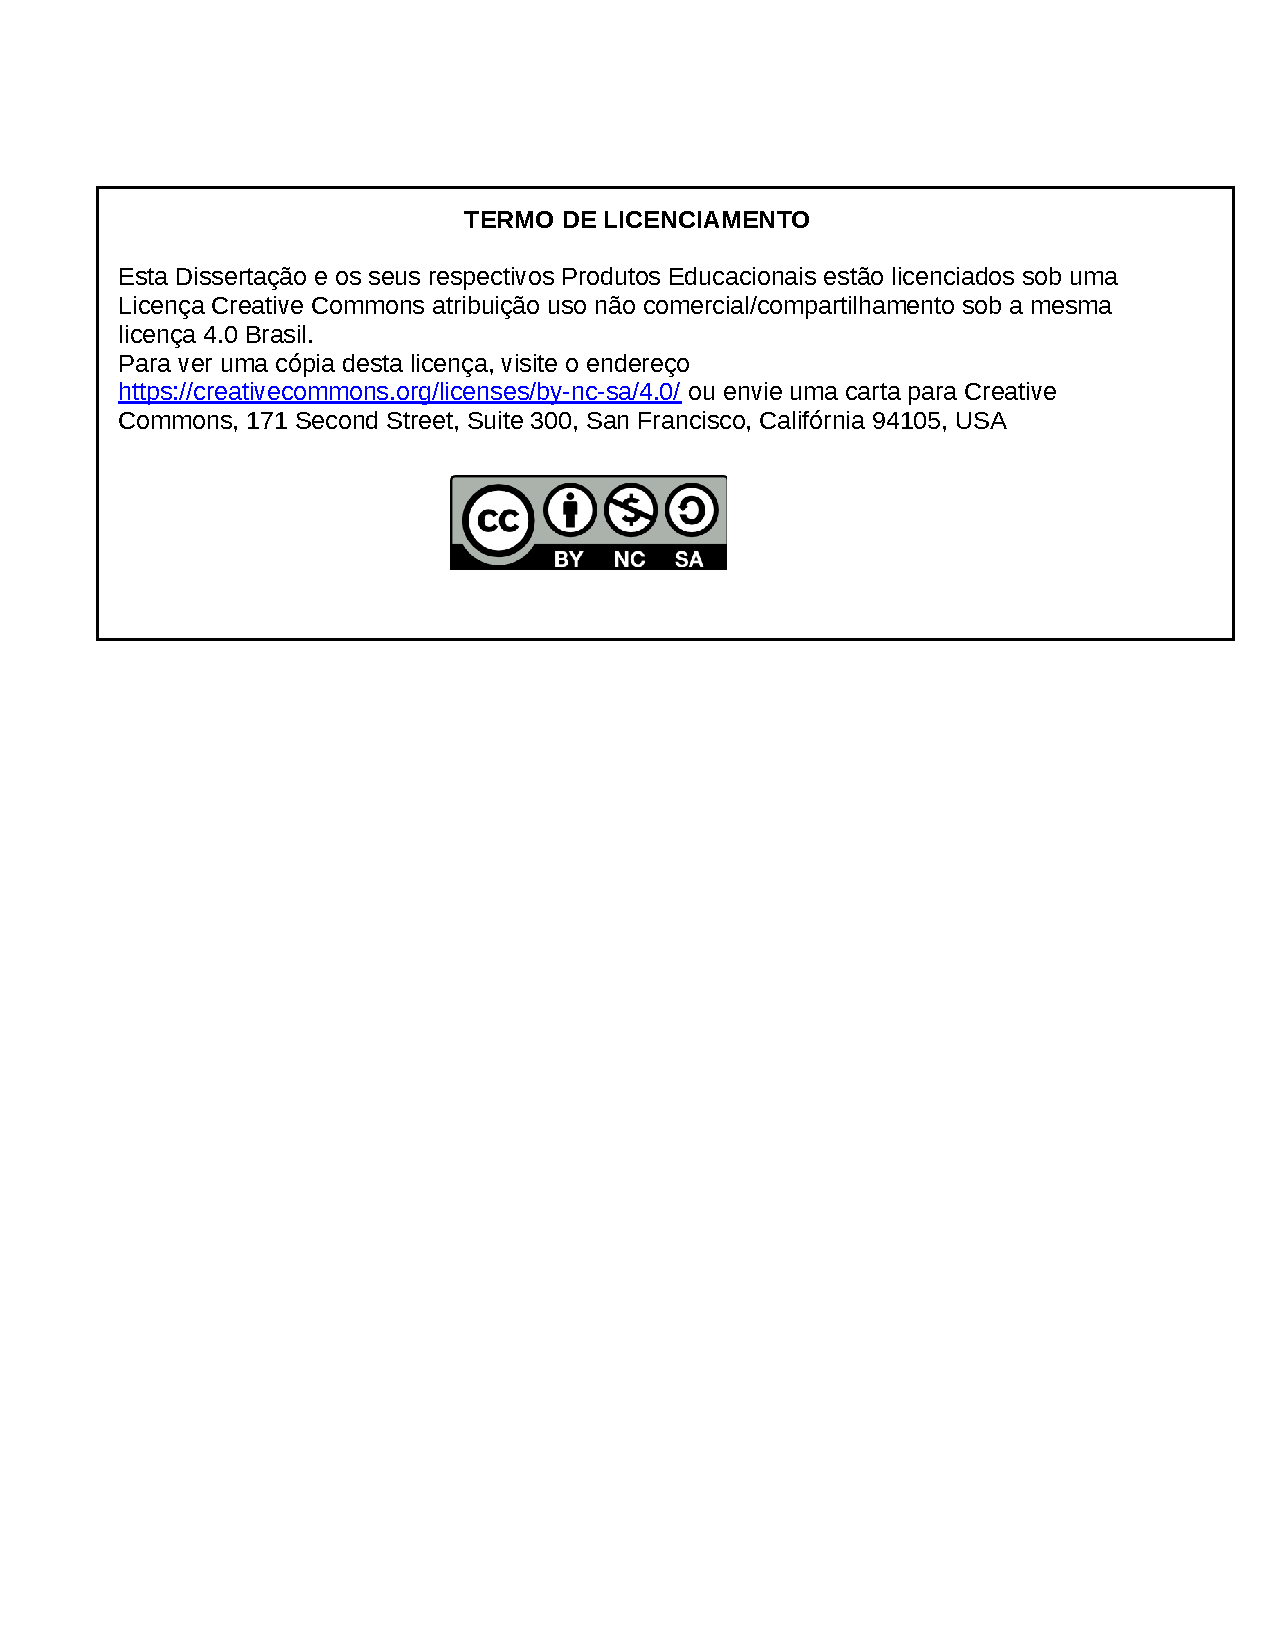
\includepdf{fichacatalografica.pdf}
			 %\end{fichacatalografica}
			 % Se voc\^e optar por elaborar a ficha catalogr\'afica, dever\'a 
			 % incluir uma % antes das 3 linhas acima e tirar a % antes
			 % do comando %% USPSC-fichacatalografica.tex
% ---
% Inserir a ficha bibliografica
% ---
% Isto \'e um exemplo de Ficha Catalogr\'afica, ou ``Dados internacionais de
% cataloga\c{c}\~ao-na-publica\c{c}\~ao''. Voc\^e pode utilizar este modelo como refer\^encia. 
% Por\'em, provavelmente a biblioteca da sua universidade lhe fornecer\'a um PDF
% com a ficha catalogr\'afica definitiva ap\'os a defesa do trabalho. Quando estiver
% com o documento, salve-o como PDF no diret\'orio do seu projeto e substitua todo
% o conte\'udo de implementa\c{c}\~ao deste arquivo pelo comando abaixo:
%
\begin{fichacatalografica}
	\hspace{-1.4cm}
	\imprimirnotaautorizacao \\ \\
	%\sffamily
	\vspace*{\fill}					% Posi\c{c}\~ao vertical
\begin{center}					% Minipage Centralizado
  \imprimirnotabib \\
  \begin{table}[htb]
	\scriptsize
	\centering	
	\begin{tabular}{|p{0.9cm} p{8.7cm}|}
		\hline
	      & \\
		  &	  \imprimirautorficha     \\
		
		 \imprimircutter & 
							\hspace{0.4cm}\imprimirtitulo~  / ~\imprimirautor~ ;  ~\imprimirorientadorcorpoficha. -- 	\imprimirlocal, \imprimirdata.   \\
		
		  &  % Para incluir nota referente \`a vers\~ao corrigida no corpo da ficha,
			  % incluir % no in\'{\i}cio da linha acima e tirar a % do in\'{\i}cio da linha abaixo
			  %	\hspace{0.4cm} \imprimirtitulo~  / ~\imprimirautor~ ; ~\imprimirorientadorcorpoficha~- ~\imprimirnotafolharosto. -- \imprimirlocal, \imprimirdata.  \\
		
			\hspace{0.4cm}\pageref{LastPage} p. : il. (algumas color.) ; 30 cm.\\ 
		  & \\
		  & 
		    \hspace{0.4cm}\imprimirnotaficha ~--~ 
						  \imprimirunidademin, 
						  \imprimiruniversidademin, 
		                  \imprimirdata. \\ 
		  & \\                 
		   % Para incluir nota referente \`a vers\~ao corrigida em notas,
		    % incluir uma % no in\'{\i}cio da linha acima e	
		    % tirar a % do in\'{\i}cio da linha abaixo
		    % & \hspace{0.4cm}\imprimirnotafolharosto \\ 
		  & \\ 
		  & \hspace{0.4cm}1. LaTeX. 2. abnTeX. 3. Classe USPSC. 4. Editora\c{c}\~ao de texto. 5. Normaliza\c{c}\~ao da documenta\c{c}\~ao. 6. Tese. 7. Disserta\c{c}\~ao. 8. Documentos (elabora\c{c}\~ao). 9. Documentos eletr\^onicos. I. \imprimirorientadorficha. 
		   II. T\'{\i}tulo. \\
	
		     %Se houver co-orientador, inclua % antes da linha (antes de II. T\'{\i}tulo.) 
		     %          e tire a % antes do comando abaixo 
		     %III. T\'{\i}tulo. \\   
		  \hline
	\end{tabular}
  \end{table}
\end{center}
\end{fichacatalografica}
% ---


			 %% USPSC-fichacatalografica.tex
% ---
% Inserir a ficha bibliografica
% ---
% Isto \'e um exemplo de Ficha Catalogr\'afica, ou ``Dados internacionais de
% cataloga\c{c}\~ao-na-publica\c{c}\~ao''. Voc\^e pode utilizar este modelo como refer\^encia. 
% Por\'em, provavelmente a biblioteca da sua universidade lhe fornecer\'a um PDF
% com a ficha catalogr\'afica definitiva ap\'os a defesa do trabalho. Quando estiver
% com o documento, salve-o como PDF no diret\'orio do seu projeto e substitua todo
% o conte\'udo de implementa\c{c}\~ao deste arquivo pelo comando abaixo:
%
\begin{fichacatalografica}
	\hspace{-1.4cm}
	\imprimirnotaautorizacao \\ \\
	%\sffamily
	\vspace*{\fill}					% Posi\c{c}\~ao vertical
\begin{center}					% Minipage Centralizado
  \imprimirnotabib \\
  \begin{table}[htb]
	\scriptsize
	\centering	
	\begin{tabular}{|p{0.9cm} p{8.7cm}|}
		\hline
	      & \\
		  &	  \imprimirautorficha     \\
		
		 \imprimircutter & 
							\hspace{0.4cm}\imprimirtitulo~  / ~\imprimirautor~ ;  ~\imprimirorientadorcorpoficha. -- 	\imprimirlocal, \imprimirdata.   \\
		
		  &  % Para incluir nota referente \`a vers\~ao corrigida no corpo da ficha,
			  % incluir % no in\'{\i}cio da linha acima e tirar a % do in\'{\i}cio da linha abaixo
			  %	\hspace{0.4cm} \imprimirtitulo~  / ~\imprimirautor~ ; ~\imprimirorientadorcorpoficha~- ~\imprimirnotafolharosto. -- \imprimirlocal, \imprimirdata.  \\
		
			\hspace{0.4cm}\pageref{LastPage} p. : il. (algumas color.) ; 30 cm.\\ 
		  & \\
		  & 
		    \hspace{0.4cm}\imprimirnotaficha ~--~ 
						  \imprimirunidademin, 
						  \imprimiruniversidademin, 
		                  \imprimirdata. \\ 
		  & \\                 
		   % Para incluir nota referente \`a vers\~ao corrigida em notas,
		    % incluir uma % no in\'{\i}cio da linha acima e	
		    % tirar a % do in\'{\i}cio da linha abaixo
		    % & \hspace{0.4cm}\imprimirnotafolharosto \\ 
		  & \\ 
		  & \hspace{0.4cm}1. LaTeX. 2. abnTeX. 3. Classe USPSC. 4. Editora\c{c}\~ao de texto. 5. Normaliza\c{c}\~ao da documenta\c{c}\~ao. 6. Tese. 7. Disserta\c{c}\~ao. 8. Documentos (elabora\c{c}\~ao). 9. Documentos eletr\^onicos. I. \imprimirorientadorficha. 
		   II. T\'{\i}tulo. \\
	
		     %Se houver co-orientador, inclua % antes da linha (antes de II. T\'{\i}tulo.) 
		     %          e tire a % antes do comando abaixo 
		     %III. T\'{\i}tulo. \\   
		  \hline
	\end{tabular}
  \end{table}
\end{center}
\end{fichacatalografica}
% ---


			 % As informa\c{c}\~oes que comp\~oem a ficha catalogr\'afica est\~ao 
			 % definidas no arquivo USPSC-pre-textual-UUUU.tex
			 % ---
			 \end{verbatim} 
			 				
\'E poss\'{\i}vel incluir ou n\~ao o C\'odigo Cutter na ficha catalogr\'afica, conforme a seguinte orienta\c{c}\~ao nos respectivos arquivos pr\'e-textuais:

\begin{verbatim}
\cutter{S856m}
% Para gerar a ficha catalogr\'afica sem o C\'odigo Cutter, basta 
% incluir uma % na linha acima e tirar a % da linha abaixo
%\cutter{ } 
\end{verbatim} 

Atrav\'es do arquivo fichacatalografica.tex \'e poss\'{\i}vel elaborar a ficha catalogr\'afica em \LaTeX\ . Caso o trabalho possua co-orientador ser\'a necess\'ario seguir as orienta\c{c}\~oes contidas tamb\'em no arquivo com os elementos pr\'e-textuais.	 


\section{Resultados de comandos}\label{sec-divisoes}

O conte\'udo desta se\c{c}\~ao foi baseado no item \textbf{1 Resultados de comandos} do \textbf{Modelo can\^onico de trabalho acad\^emico com abnTEX2} \cite{equipeabntex2}.

% ---
\subsection{Codifica\c{c}\~ao dos arquivos: UTF8}
% ---

A codifica\c{c}\~ao \texttt{UTF8} deve ser utilizada para todos os arquivos do \abnTeX\ . Utilize a mesma codifica\c{c}\~ao nos documentos que escrever, incluindo nos arquivos de bases bibliogr\'aficas |.bib|. Para tanto, tanto o arquivo USPSC-modelo.tex  quanto o USPSC-TCC-modelo.tex devem conter o seguinte pacote:

\begin{verbatim}
\usepackage[utf8]{inputenc}	 % Codificacao do documento (convers\~ao
                               autom\'atica dos acentos)
\end{verbatim}

% ---
\subsection{Diferentes idiomas e hifeniza\c{c}\~oes}
\label{sec-hifenizacao}
% ---

Para usar hifeniza\c{c}\~oes de diferentes idiomas, inclua nas op\c{c}\~oes do documento o
nome dos idiomas que o seu texto cont\'em. Os usu\'arios da Classe USPSC devem utilizar:

\begin{verbatim}
\documentclass[
% -- op\c{c}\~oes da classe memoir --
12pt,		% tamanho da fonte
openright,	% cap\'{\i}tulos come\c{c}am em p\'ag \'{\i}mpar (insere p\'agina vazia caso 
preciso)
twoside,  % para impress\~ao em anverso (frente) e verso. Oposto a oneside - 
Nota: utilizar \imprimirfolhaderosto*
%oneside, % para impress\~ao em p\'aginas separadas (somente anverso) -  
Nota: utilizar \imprimirfolhaderosto
% inclua uma % antes do comando twoside e exclua a % antes do oneside 
a4paper,			% tamanho do papel. 
% -- op\c{c}\~oes da classe abntex2 --
chapter=TITLE,		% t\'{\i}tulos de cap\'{\i}tulos convertidos em letras 
mai\'usculas
% -- op\c{c}\~oes do pacote babel --
english,			% idioma adicional para hifeniza\c{c}\~ao
french,				% idioma adicional para hifeniza\c{c}\~ao
spanish,			% idioma adicional para hifeniza\c{c}\~ao
brazil				% o \'ultimo idioma \'e o principal do documento
% {USPSC-classe/USPSC} configura o cabe\c{c}alho contendo apenas o n\'umero 
da p\'agina
]{USPSC-classe/USPSC}
%]{USPSC-classe/USPSC1}
% Inclua % antes de ]{USPSC-classe/USPSC} e retire a % antes 
de %]{USPSC-classe/USPSC1} para utilizar o 
% cabe\c{c}alho diferenciado para as p\'aginas pares e \'{\i}mpares:
%- p\'aginas \'{\i}mpares: cabe\c{c}alho com se\c{c}\~oes ou subse\c{c}\~oes e o n\'umero da p\'agina
%- p\'aginas pares: cabe\c{c}alho com o n\'umero da p\'agina e o t\'{\i}tulo do cap\'{\i}tulo 
% ---
\end{verbatim}

Desta forma o texto dever\'a ser escrito idioma portugu\^es-brasileiro (\texttt{brazil}), podendo ter cita\c{c}\~oes em ingl\^es, franc\^es e espanhol.

O idioma portugu\^es-brasileiro (\texttt{brazil}) \'e inclu\'{\i}do automaticamente pela
classe \textsf{abntex2}. Por\'em, mesmo assim a op\c{c}\~ao \texttt{brazil} deve ser
informada como a \'ultima op\c{c}\~ao da classe para que todos os pacotes reconhe\c{c}am o
idioma. Vale ressaltar que a \'ultima op\c{c}\~ao de idioma \'e a utilizada por padr\~ao no
documento. 

Portanto, para Classe USPSC, caso deseje escrever um texto em ingl\^es que tenha
cita\c{c}\~oes em espanhol, portugu\^es e franc\^es, voc\^e dever\'a usar:

\begin{verbatim}
\documentclass[
% -- op\c{c}\~oes da classe memoir --
12pt,		% tamanho da fonte
openright,	% cap\'{\i}tulos come\c{c}am em p\'ag \'{\i}mpar (insere p\'agina vazia caso 
preciso)
twoside,  % para impress\~ao em anverso (frente) e verso. Oposto a oneside - 
Nota: utilizar \imprimirfolhaderosto*
%oneside, % para impress\~ao em p\'aginas separadas (somente anverso) -  
Nota: utilizar \imprimirfolhaderosto
% inclua uma % antes do comando twoside e exclua a % antes do oneside 
a4paper,			% tamanho do papel. 
% -- op\c{c}\~oes da classe abntex2 --
chapter=TITLE,		% t\'{\i}tulos de cap\'{\i}tulos convertidos em letras 
mai\'usculas
% -- op\c{c}\~oes do pacote babel --
spanish,			% idioma adicional para hifeniza\c{c}\~ao
french,				% idioma adicional para hifeniza\c{c}\~ao
brazil,				% o \'ultimo idioma \'e o principal do documento
english 			% idioma adicional para hifeniza\c{c}\~ao
% {USPSC-classe/USPSC} configura o cabe\c{c}alho contendo apenas o n\'umero 
da p\'agina
]{USPSC-classe/USPSC}
%]{USPSC-classe/USPSC1}
% Inclua % antes de ]{USPSC-classe/USPSC} e retire a % antes 
de %]{USPSC-classe/USPSC1} para utilizar o 
% cabe\c{c}alho diferenciado para as p\'aginas pares e \'{\i}mpares:
%- p\'aginas \'{\i}mpares: cabe\c{c}alho com se\c{c}\~oes ou subse\c{c}\~oes e o n\'umero da p\'agina
%- p\'aginas pares: cabe\c{c}alho com o n\'umero da p\'agina e o t\'{\i}tulo do cap\'{\i}tulo 
% ---
\end{verbatim}

A lista completa de idiomas suportados, bem como outras op\c{c}\~oes de hifeniza\c{c}\~ao,
est\~ao dispon\'{\i}veis em \citeonline[p.~7-8]{babel2011}. \\

Exemplo de hifeniza\c{c}\~ao em ingl\^es\footnote{Extra\'{\i}do de:
	\url{http://en.wikibooks.org/wiki/LaTeX/Internationalization}}:

\begin{otherlanguage*}{english}
	\textit{Text in English language. This environment switches all language-related
		definitions, like the language specific names for figures, tables etc. to the other
		language. The starred version of this environment typesets the main text
		according to the rules of the other language, but keeps the language specific
		string for ancillary things like figures, in the main language of the document.
		The environment hyphenrules switches only the hyphenation patterns used; it can
		also be used to disallow hyphenation by using the language name
		`nohyphenation'.}
\end{otherlanguage*}

Exemplo de hifeniza\c{c}\~ao em franc\^es\footnote{Extra\'{\i}do de:
	\url{http://bigbrowser.blog.lemonde.fr/2013/02/17/tu-ne-tweeteras-point-le-vatican-interdit-aux-cardinaux-de-tweeter-pendant-le-conclave/}}:

\begin{otherlanguage*}{french}
	\textit{Texte en fran\c{c}ais. Pas question que Twitter ne vienne faire une
		concurrence d\'eloyale \`a la traditionnelle fum\'ee blanche qui marque l'\'election
		d'un nouveau pape. Pour \'eviter toute fuite pr\'ecoce, le Vatican a donc pris un
		peu d'avance, et a d\'ej\`a interdit aux cardinaux qui prendront part au vote
		d'utiliser le r\'eseau social, selon Catholic News Service. Une mesure valable
		surtout pour les neuf cardinaux – sur les 117 du conclave – pratiquants très
		actifs de Twitter, qui auront interdiction pendant toute la p\'eriode de se
		connecter \`a leur compte.}
\end{otherlanguage*}

Exemplo de hifeniza\c{c}\~ao em espanhol\footnote{Extra\'{\i}do de:
	\url{http://internacional.elpais.com/internacional/2013/02/17/actualidad/1361102009_913423.html}}:

\foreignlanguage{spanish}{\textit{Decenas de miles de personas ovacionan al pont\'{\i}fice en su
		pen\'ultimo \'angelus dominical, el primero desde que anunciase su renuncia. El Papa se
		centra en la cr\'{\i}tica al materialismo}}.

O idioma geral do texto pode ser alterado como no exemplo seguinte:

\begin{verbatim}
\selectlanguage{english}

\end{verbatim}

Isso altera automaticamente a hifeniza\c{c}\~ao e todos os nomes constantes de
refer\^encias do documento para o idioma ingl\^es. Consulte o manual da classe para obter orienta\c{c}\~oes adicionais sobre internacionaliza\c{c}\~ao de documentos produzidos com \textsf{\abnTeX} \cite{abnetxclasse}.

Se a op\c{c}\~ao de idioma do texto n\~ao for o portugu\^es, \'e necess\'ario observar o descrito em \ref{idioma}.

% ---
\subsection{Enumera\c{c}\~oes}
% ---

\index{al\'{\i}neas}\index{subal\'{\i}neas}\index{incisos}Quando for necess\'ario enumerar
os diversos assuntos de uma se\c{c}\~ao que n\~ao possua t\'{\i}tulo, esta deve ser
subdividida em al\'{\i}neas \cite[4.2]{nbr6024}:

\begin{alineas}

  \item os diversos assuntos que n\~ao possuam t\'{\i}tulo pr\'oprio, dentro de uma mesma
  se\c{c}\~ao, devem ser subdivididos em al\'{\i}neas; 
  
  \item o texto que antecede as al\'{\i}neas termina em dois pontos;
  \item as al\'{\i}neas devem ser indicadas alfabeticamente, em letra min\'uscula
  seguida de par\^entese. Utilizam-se letras dobradas, quando esgotadas as
  letras do alfabeto;

  \item as letras indicativas das al\'{\i}neas devem apresentar recuo em rela\c{c}\~ao \`a
  margem esquerda;

  \item o texto da al\'{\i}nea deve come\c{c}ar por letra min\'uscula e terminar em
  ponto-e-v\'{\i}rgula, exceto a \'ultima al\'{\i}nea que termina em ponto final;

  \item o texto da al\'{\i}nea deve terminar em dois pontos, se houver subal\'{\i}nea;

  \item a segunda e as seguintes linhas do texto da al\'{\i}nea come\c{c}a sob a
  primeira letra do texto da pr\'opria al\'{\i}nea;
  
  \item subal\'{\i}neas \cite{nbr6024} devem ser conforme as al\'{\i}neas a
  seguir:

  \begin{alineas}
     \item as subal\'{\i}neas devem come\c{c}ar por travess\~ao seguido de espa\c{c}o;

     \item as subal\'{\i}neas devem apresentar recuo em rela\c{c}\~ao \`a al\'{\i}nea;

     \item o texto da subal\'{\i}nea deve come\c{c}ar por letra min\'uscula e terminar em
     ponto-e-v\'{\i}rgula. A \'ultima subal\'{\i}nea deve terminar em ponto final, se n\~ao
     houver al\'{\i}nea subsequente;

     \item a segunda e as seguintes linhas do texto da subal\'{\i}nea come\c{c}am sob a
     primeira letra do texto da pr\'opria subal\'{\i}nea.
  \end{alineas}
  
  \item no \abnTeX\ est\~ao dispon\'{\i}veis os ambientes \texttt{incisos} e
  \texttt{subalineas}, que em suma \'e o mesmo que se criar outro n\'{\i}vel de
  \texttt{alineas}, como nos exemplos \`a seguir:
  
  \begin{incisos}
    \item \textit{Um novo inciso em it\'alico};
  \end{incisos}
  
  \item Al\'{\i}nea em \textbf{negrito}:
  
  \begin{subalineas}
    \item \textit{Uma subal\'{\i}nea em it\'alico};
    \item \underline{\textit{Uma subal\'{\i}nea em it\'alico e sublinhado}}; 
  \end{subalineas}
  
  \item \'Ultima al\'{\i}nea com \emph{\^enfase}.
  
\end{alineas}

% ---
\subsection{Espa\c{c}amento entre par\'agrafos e linhas}\label{sec_espacamento}
% ---

\index{espa\c{c}amento!dos par\'agrafos}O tamanho do par\'agrafo, espa\c{c}o entre a margem
e o in\'{\i}cio da frase do par\'agrafo, \'e definido por:

\begin{verbatim}
   \setlength{\parindent}{1.3cm}
\end{verbatim}

\index{espa\c{c}amento!do primeiro par\'agrafo}Por padr\~ao, n\~ao h\'a espa\c{c}amento no
primeiro par\'agrafo de cada in\'{\i}cio de divis\~ao do documento
(\autoref{sec-divisoes-b}). Por\'em, voc\^e pode definir que o primeiro par\'agrafo
tamb\'em seja indentado, como \'e o caso deste documento. Para isso, apenas inclua o
pacote \textsf{indentfirst} no pre\^ambulo do documento:

\begin{verbatim}
   \usepackage{indentfirst} % Indenta o primeiro par\'agrafo de cada se\c{c}\~ao.
\end{verbatim}

\index{espa\c{c}amento!entre os par\'agrafos}O espa\c{c}amento entre um par\'agrafo e outro
pode ser controlado por meio do comando:

\begin{verbatim}
  \setlength{\parskip}{0.2cm}  % tente tamb\'em \onelineskip
\end{verbatim}

\index{espa\c{c}amento!entre as linhas}O controle do espa\c{c}amento entre linhas \'e
definido por:
\begin{verbatim}
  \OnehalfSpacing       % espa\c{c}amento um e meio (padr\~ao); 
  \DoubleSpacing        % espa\c{c}amento duplo
  \SingleSpacing        % espa\c{c}amento simples	
\end{verbatim}

Para isso, tamb\'em est\~ao dispon\'{\i}veis os ambientes:
\begin{verbatim}
  \begin{SingleSpace} ...\end{SingleSpace}
  \begin{Spacing}{hfactori} ... \end{Spacing}
  \begin{OnehalfSpace} ... \end{OnehalfSpace}
  \begin{OnehalfSpace*} ... \end{OnehalfSpace*}
  \begin{DoubleSpace} ... \end{DoubleSpace}
  \begin{DoubleSpace*} ... \end{DoubleSpace*} 
\end{verbatim}

% ---
\subsection{Tabelas e quadros}

As tabelas e os quadros apresentam os dados de modo resumido, oferecendo uma vis\~ao geral do conte\'udo em quest\~ao, visando facilitar a compreens\~ao do fen\^omeno em estudo. A diferen\c{c}a b\'asica entre ambas est\'a relacionada ao conte\'udo e a formata\c{c}\~ao. 

Tabela \'e o conjunto de dados estat\'{\i}sticos, dispostos em determinada ordem de classifica\c{c}\~ao, que expressam as varia\c{c}\~oes qualitativas de um fen\^omeno. Sua finalidade b\'asica \'e resumir ou sintetizar dados \cite{sibi2016}.

A constru\c{c}\~ao de tabelas deve obedecer os crit\'erios estabelecidos pelo Instituto Brasileiro de Geografia e Estat\'{\i}stica (IBGE) e requeridos pelas normas da ABNT para documentos t\'ecnicos e acad\^emicos.

A \autoref{tab-ibge} \'e um exemplo de tabela alinhada que pode ser longa ou curta, conforme padr\~ao do IBGE.

\begin{table}[htb]
	%\begin{table}[H]
	\IBGEtab{%
		\caption{Frequ\^encia anual por categoria de usu\'arios}%
		\label{tab-ibge}
	}{%
	\begin{tabular}{ccc}
		\toprule
		Categoria de Usu\'arios & Frequ\^encia de Usu\'arios \\
		\midrule \midrule
		Gradua\c{c}\~ao & 72\% \\
		\midrule 
		P\'os-Gradua\c{c}\~ao & 15\% \\
		\midrule 
		Docente & 10\% \\
		\midrule 
		Outras & 3\% \\
		\bottomrule
	\end{tabular}%
}{%
\fonte{Elaborada pelos autores.}%
\nota{Exemplo de uma nota.}%
\nota[Anota\c{c}\~oes]{Uma anota\c{c}\~ao adicional, que pode ser seguida de v\'arias
	outras.}%

}
\end{table}


\begin{table}[H]
	\IBGEtab{%
		\caption{N\'{\i}veis descritivos dos testes de compara\c{c}\~ao de m\'edias entre grupos para profundidade da les\~ao junto \`a restaura\c{c}\~ao}%
		\label{tabela-ibge}
	}{%
	\begin{tabular}{p{5.5cm}|p{5.5cm}}
		\hline
		\textbf{Resultado} & \textbf{N\'{\i}vel Descritivo} \\ 
		\hline 
		CIC < Ariston & < 0,0001  \\
		Ariston < Am & 0,0118  \\
		Am = Helio & 0,4576  \\
		-100 = Helio & 0,3360  \\
		\hline
	\end{tabular}%
}{%
\fonte{\citeonline{sibi2009}}%
}
\end{table} 

Os \textbf{AP\^ENDICES J-K} exemplificam outras formata\c{c}\~oes de tabelas.

A formata\c{c}\~ao do quadro \'e similar \`a tabela, mas deve ter suas laterais fechadas e conter as linhas horizontais.

% o comando \newpage foi utilizado para for\c{c}ar a quebra de p\'agina

\begin{quadro}[htb]
	\caption{\label{quadro_modelo}N\'{\i}veis de investiga\c{c}\~ao}
	\begin{tabular}{|p{2.6cm}|p{6.0cm}|p{2.25cm}|p{3.40cm}|}
		\hline
		\textbf{N\'{\i}vel de Investiga\c{c}\~ao} & \textbf{Insumos}  & \textbf{Sistemas de Investiga\c{c}\~ao}  & \textbf{Produtos}  \\
		\hline
		Meta-n\'{\i}vel & Filosofia\index{filosofia} da Ci\^encia  & Epistemologia &
		Paradigma  \\
		\hline
		N\'{\i}vel do objeto & Paradigmas do metan\'{\i}vel e evid\^encias do n\'{\i}vel inferior &
		Ci\^encia  & Teorias e modelos \\
		\hline
		N\'{\i}vel inferior & Modelos e m\'etodos do n\'{\i}vel do objeto e problemas do n\'{\i}vel inferior & Pr\'atica & Solu\c{c}\~ao de problemas  \\
		\hline
	\end{tabular}
	\begin{flushleft}
		%\fonte{\citeonline{van1986}}
		Fonte: \citeonline{van1986}
	\end{flushleft}
\end{quadro} 


Os \textbf{AP\^ENDICES B-I} apresentam exemplos de quadros.

% ---
\subsection{Figuras}\label{sec_figuras}
% ---
\index{figuras}Figuras podem ser criadas diretamente em \LaTeX,
como o exemplo da \autoref{fig_circulo}. \\ 

\begin{figure}[htb]
	\caption{\label{fig_circulo}A delimita\c{c}\~ao do espa\c{c}o}
	\begin{center}
		\setlength{\unitlength}{9cm}
		\begin{picture}(1,1)
		\put(0,0){\line(0,1){1}}
		\put(0,0){\line(1,0){1}}
		\put(0,0){\line(1,1){1}}
		\put(0,0){\line(1,2){.5}}
		\put(0,0){\line(1,3){.3333}}
		\put(0,0){\line(1,4){.25}}
		\put(0,0){\line(1,5){.2}}
		\put(0,0){\line(1,6){.1667}}
		\put(0,0){\line(2,1){1}}
		\put(0,0){\line(2,3){.6667}}
		\put(0,0){\line(2,5){.4}}
		\put(0,0){\line(3,1){1}}
		\put(0,0){\line(3,2){1}}
		\put(0,0){\line(3,4){.75}}
		\put(0,0){\line(3,5){.6}}
		\put(0,0){\line(4,1){1}}
		\put(0,0){\line(4,3){1}}
		\put(0,0){\line(4,5){.8}}
		\put(0,0){\line(5,1){1}}
		\put(0,0){\line(5,2){1}}
		\put(0,0){\line(5,3){1}}
		\put(0,0){\line(5,4){1}}
		\put(0,0){\line(5,6){.8333}}
		\put(0,0){\line(6,1){1}}
		\put(0,0){\line(6,5){1}}
		\end{picture}
	\end{center}
	\legend{Fonte: \citeonline{equipeabntex2}}
\end{figure}

Outra op\c{c}\~ao \'e incorporar a figura utilizando um arquivo externo, como \'e o caso da \autoref{fig_grafico}. Se a figura que for inclu\'{\i}da se tratar de um diagrama, um gr\'afico ou uma ilustra\c{c}\~ao, que voc\^e mesmo produza, priorize o uso de imagens vetoriais no formato PDF. Com isso, o tamanho do arquivo final do trabalho ser\'a menor e as imagens ter\~ao uma apresenta\c{c}\~ao melhor, principalmente quando impressas, uma vez que imagens vetoriais s\~ao perfeitamente escal\'aveis para qualquer dimens\~ao. Nesse caso, se for utilizar o Microsoft Excel para produzir gr\'aficos, ou o Microsoft Word para ilustra\c{c}\~oes, exporte-os como PDF e os incorpore ao documento conforme o exemplo abaixo. No entanto, para manter a
coer\^encia no uso de software livre (j\'a que voc\^e est\'a usando \LaTeX\  e \abnTeX),
teste a ferramenta \textsf{InkScape}\index{InkScape}
(\url{http://inkscape.org/}). Ela \'e uma excelente op\c{c}\~ao de c\'odigo-livre para
produzir ilustra\c{c}\~oes vetoriais, similar ao CorelDraw\index{CorelDraw} ou ao Adobe
Illustrator\index{Adobe Illustrator}. De todo modo, caso n\~ao seja poss\'{\i}vel
utilizar arquivos de imagens como PDF, utilize qualquer outro formato, como
JPEG, GIF, BMP, etc. Nesse caso, voc\^e pode tentar aprimorar as imagens
incorporadas com o software livre \textsf{Gimp}\index{Gimp}
(\url{http://www.gimp.org/}). Ele \'e uma alternativa livre ao Adobe
Photoshop\index{Adobe Photoshop}. \\

\begin{figure}[H]
	\caption{\label{fig_grafico}Gr\'afico produzido em Excel e salvo como PDF}
	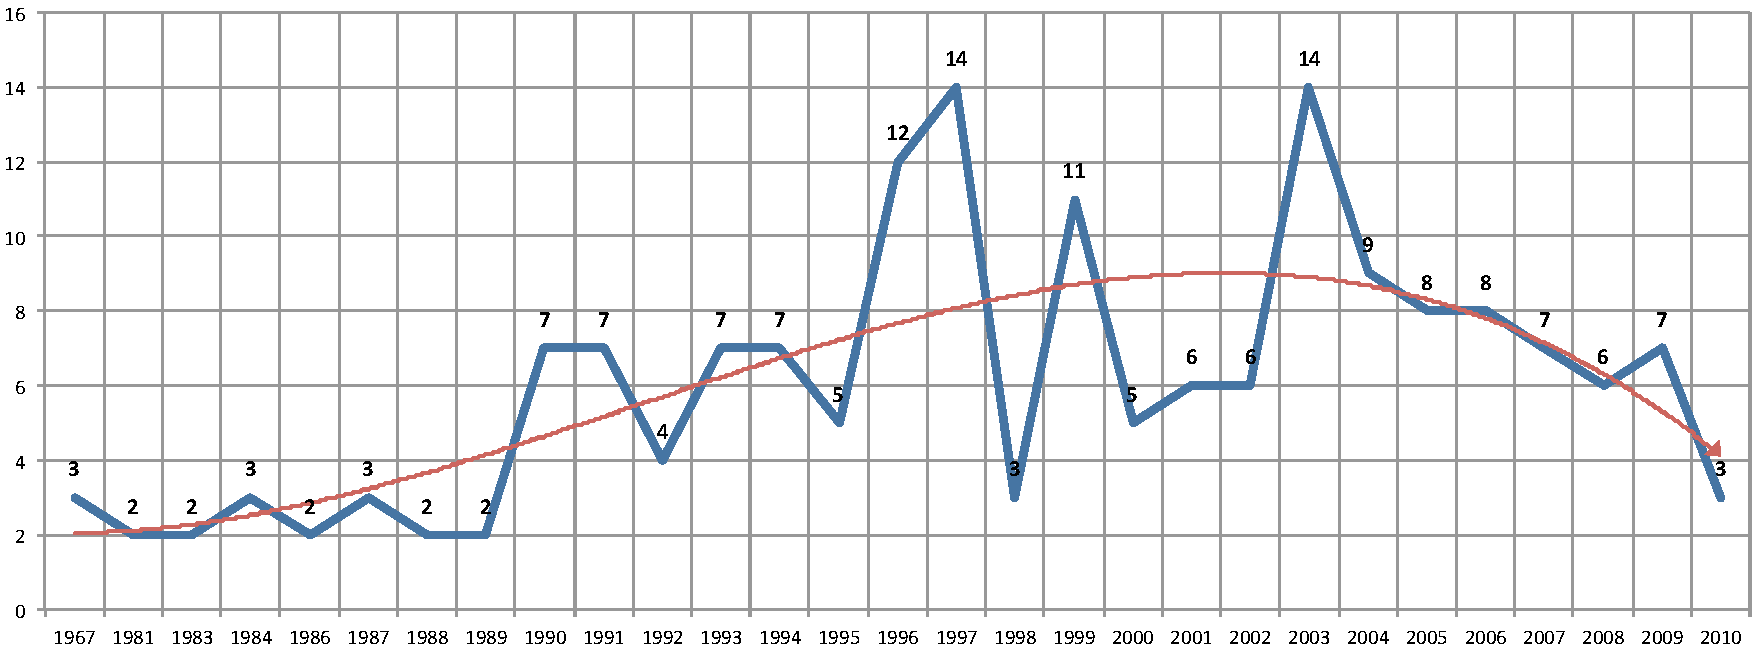
\includegraphics[scale=0.5]{USPSC-img/USPSC-modelo-img-grafico.pdf}
	\begin{flushleft}
		Fonte: \citeonline[p. 24]{araujo2012}
	\end{flushleft}	
\end{figure}

% ---
\subsubsection{Figuras em minipages}
% ---

As ilustra\c{c}\~oes devem sempre ter numera\c{c}\~ao cont\'{\i}nua e \'unica em todo o documento:

% O comando \newpage for\c{c}a a quebra de p\'agina

\begin{citacao}
	Qualquer que seja o tipo de ilustra\c{c}\~ao, sua identifica\c{c}\~ao aparece na parte
	superior, precedida da palavra designativa (desenho, esquema, fluxograma,
	fotografia, gr\'afico, mapa, organograma, planta, quadro, retrato, figura,
	imagem, entre outros), seguida de seu n\'umero de ordem de ocorr\^encia no texto,
	em algarismos ar\'abicos, travess\~ao e do respectivo t\'{\i}tulo. Ap\'os a ilustra\c{c}\~ao, na
	parte inferior, indicar a fonte consultada (elemento obrigat\'orio, mesmo que
	seja produ\c{c}\~ao do pr\'oprio autor), legenda, notas e outras informa\c{c}\~oes
	necess\'arias \`a sua compreens\~ao (se houver). A ilustra\c{c}\~ao deve ser citada no
	texto e inserida o mais pr\'oximo poss\'{\i}vel do trecho a que se
	refere \cite{nbr14724}.
\end{citacao}

\emph{Minipages} s\~ao usadas para inserir textos ou outros elementos em quadros
com tamanhos e posi\c{c}\~oes controladas. Veja o exemplo da
\autoref{fig_minipage_imagem1} e da \autoref{fig_minipage_grafico2}.

\begin{figure}[H]
	\label{teste}
	\centering
	\begin{minipage}{0.4\textwidth}
		\centering
		\caption{Imagem 1 da minipage} \label{fig_minipage_imagem1}
		
\includegraphics[scale=0.9]{USPSC-img/USPSC-modelo-img-marca.pdf}
		\legend{Fonte: \citeonline{equipeabntex2}}
	\end{minipage}
	\hfill
	\begin{minipage}{0.4\textwidth}
		\centering
		\caption{Grafico 2 da minipage} \label{fig_minipage_grafico2}
		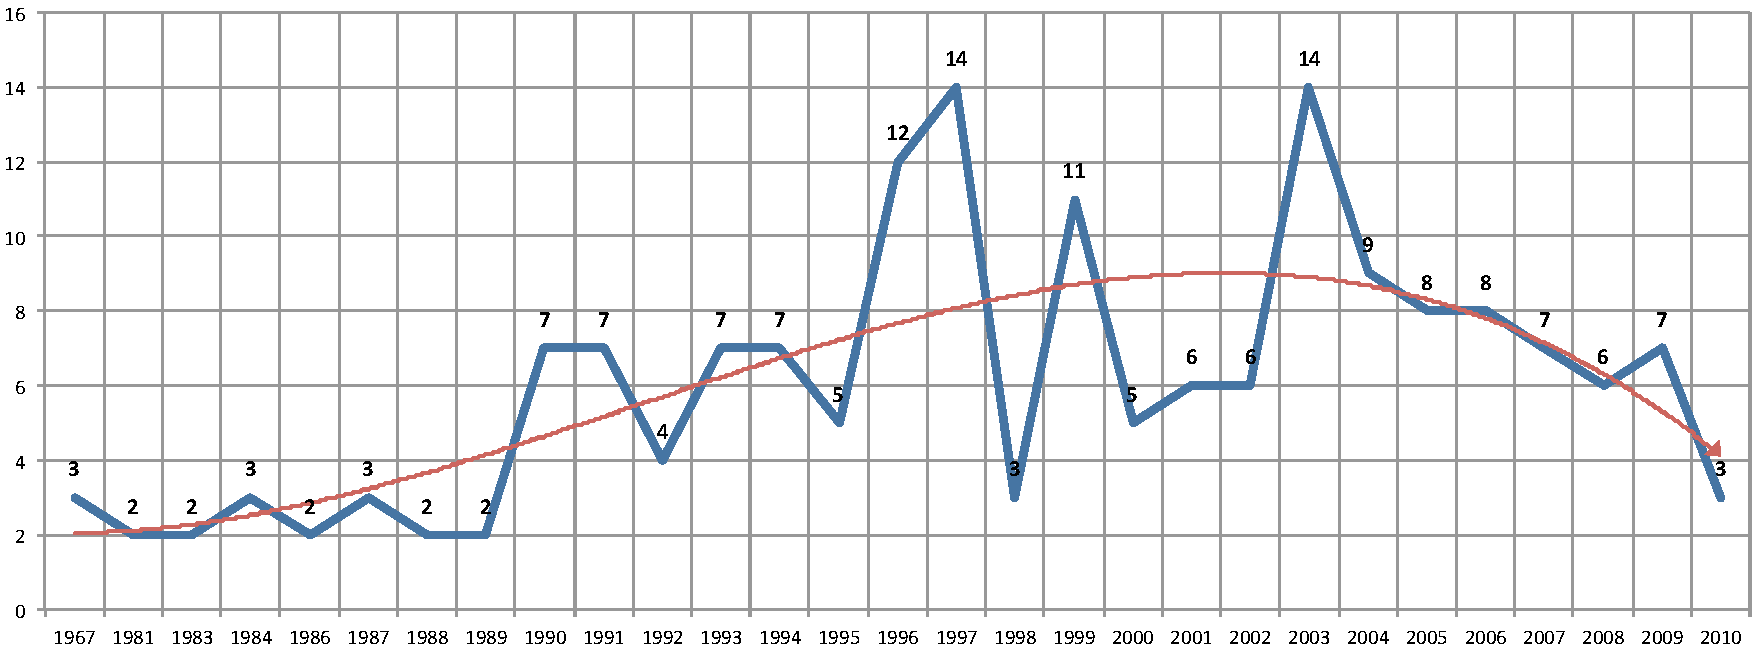
\includegraphics[scale=0.2]{USPSC-img/USPSC-modelo-img-grafico.pdf}
		\legend{Fonte: \citeonline[p. 24]{araujo2012}}
	\end{minipage}
\end{figure}

% ---
\subsection{Express\~oes matem\'aticas}
% ---

\index{express\~oes matem\'aticas}Use o ambiente \texttt{equation} para escrever
express\~oes matem\'aticas numeradas:

\begin{equation}
\forall x \in X, \quad \exists \: y \leq \epsilon
\end{equation}

Escreva express\~oes matem\'aticas entre \$ e \$, como em $ \lim_{x \to \infty}
\exp(-x) = 0 $, para que fiquem na mesma linha.

Tamb\'em \'e poss\'{\i}vel usar colchetes para indicar o in\'{\i}cio de uma express\~ao
matem\'atica que n\~ao \'e numerada.

\[
\left|\sum_{i=1}^n a_ib_i\right|
\le
\left(\sum_{i=1}^n a_i^2\right)^{1/2}
\left(\sum_{i=1}^n b_i^2\right)^{1/2}
\]

Consulte mais informa\c{c}\~oes sobre express\~oes matem\'aticas em
\url{https://github.com/abntex/abntex2/wiki/Referencias}.

\subsection{Estruturas, rea\c{c}\~oes e mecanismos de rea\c{c}\~oes qu\'{\i}micas}\label{Reaquimica}
Para a vers\~ao 3.0 do Pacote USPSC, o Grupo Desenvolvedor optou por utilizar os pacotes \textbf{mychemistry},  \textbf{ChemFig} e o \textbf{TikZ}, que fornecem comandos que permitem compor esquemas complexos de rea\c{c}\~ao qu\'{\i}mica com \LaTeX\ . 

Aqui s\~ao apresentados alguns exemplos, sendo que a maioria foram retirados do manual do pacote \textbf{ChemFig}\cite{ChemFigPac}. 


A f\'ormula estrutural do metano \'e:


\chemfig{C(-[5]H)(-[2]H)(<[:-70]H)(<:[:-20]H)} \\

\begin{verbatim}
\end{verbatim} 

Molecula da Adrenalina \'e:

\chemfig{*6((-HO)-=-(-(<[::60]OH)-[::-60]-[::-60,,,2]
	HN-[::+60]CH_3)=-(-HO)=)} \\

\begin{verbatim}
\end{verbatim}

Com o comando abaixo, o \textbf{ChemFig} possibilita escrever o nome de uma mol\'ecula abaixo dela. 

\begin{verbatim}
\ chemname [hdimi] {\ chemfig {c\'odigo da mol\'ecula}} {hnamei}
\end{verbatim}

Para exemplificar apresentamos uma rea\c{c}\~ao com os nomes das respectivas mol\'eculas:

\schemestart
\chemname{\chemfig{R-C(-[:-30]OH)=[:30]O}}{\'Acido carbox\'{\i}lico}
\+
\chemname{\chemfig{R’OH}}{\'Alcool}
\arrow(.mid east--.mid west)
\chemname{\chemfig{R-C(-[:-30]OR’)=[:30]O}}{\'Ester}
\+
\chemname{\chemfig{H_2O}}{\'Agua}
\schemestop
\chemnameinit{}
 \\

\begin{verbatim}
\end{verbatim}

Mediante a utiliza\c{c}\~ao dos pacotes \textbf{TikZ} e \textbf{ChemFig}, o pacote \textbf{xcolor} \'e carregado possibilitando o uso de cores nos c\'odigos de comandos, conforme exemplos abaixo:

\chemfig{C|{\color{blue}H_3}-C(=[1]O)-[7]O|{\color{red}H}} 

\begin{verbatim}
\end{verbatim}

Para destacar subst\^ancias individualmente ou parte de um esquema, \'e poss\'{\i}vel utilizar recursos tais como os exemplificados a seguir.

\begin{verbatim}
setchemfig{compound style={draw,line width=0.8pt,
semitransparent,text opacity=1,inner sep=8pt,
rounded corners=1mm}}
\schemestart
A\arrow([fill=red]--[fill=blue])[90]
B\arrow(--[fill=gray])
C\arrow(--[fill=green])[-90]
D\arrow(--[draw=none])[-180]
\schemestop
\end{verbatim} 

\begin{verbatim}
\end{verbatim}



\setchemfig{compound style={draw,line width=0.8pt,
		semitransparent,text opacity=1,inner sep=8pt,
		rounded corners=1mm}}
\schemestart
A\arrow([fill=red]--[fill=blue])[90]
B\arrow(--[fill=gray])
C\arrow(--[fill=green])[-90]
D\arrow(--[draw=none])[-180]
\schemestop

\begin{verbatim}
\end{verbatim} 

Mais um exemplo de utiliza\c{c}\~ao dos recursos do pacote TikZ \'e o desenho de duas linhas e um ponto de interse\c{c}\~ao. O comando \verb+ \draw[blue, thick] + define um elemento gr\'afico cuja cor \'e azul e com um tra\c{c}o grosso. A linha \'e definida por seus dois pontos finais, (-1,2) e (2, -4), unidos por -. O comando \verb+ \filldraw[red] (0,0) circle (2pt) + \\ \verb+node[anchor=west] {Intersection point} + ir\'a desenhar um c\'{\i}rculo preenchido com a cor vermelha, sendo que (0,0) define o ponto central, (2pt) determina o raio e, pr\'oximo ao ponto, um n\'o e uma caixa contendo o texto "ponto de interse\c{c}\~ao", ancorado a oeste do ponto.


\begin{verbatim}
\begin{tikzpicture}
\draw[blue, thick] (-1,2) -- (2,-4);
\draw[green, thick] (-1,-1) -- (2,2);
\filldraw[red] (0,0) circle (2pt) node[anchor=west] {Intersection point};
\end{tikzpicture}
\end{verbatim}

Tais comandos geram os elementos gr\'aficos abaixo:

\begin{tikzpicture}
\draw[blue, thick] (-1,2) -- (2,-4);
\draw[blue, thick] (-1,-1) -- (2,2);
\filldraw[red] (0,0) circle (2pt) node[anchor=west] {Intersection point};
\end{tikzpicture}


Para gerar este documento, no pre\^ambulo do arquivo principal (USPSC-modelo.tex e USPSC-TCC-modelo.tex ) foram inclu\'{\i}dos os seguintes comandos:
\begin{verbatim}
\usepackage{float} 				% Fixa tabelas e figuras no local exato
\usepackage{chemfig,chemmacros} % Para escrever rea\c{c}\~oes qu\'{\i}micas
\usepackage{mychemistry}        % Para escrever rea\c{c}\~oes qu\'{\i}micas
\usepackage{tikz}               % Para escrever rea\c{c}\~oes qu\'{\i}micas e outros
\usetikzlibrary{arrows, babel}	% Para escrever rea\c{c}\~oes qu\'{\i}micas e outros
\end{verbatim}

Para informa\c{c}\~oes complementares e recursos adicionais, consulte os manuais dos pacotes utilizados:  \textbf{mychemistry}\cite{mychemistryPac}, \textbf{ChemFig}\cite{ChemFigPac}, \textbf{etoolbox}\cite{etoolboxPack}, \textbf{float}\cite{floatPac}, \textbf{xkeyval}\cite{xkeyvalPac}, \textbf{chemmacros}\cite{chemmacrosPac}, \textbf{TikZ e PGF}\cite{TikZPac} ou de outros necess\'arios para o seu documento.


% ---
\subsection{Inclus\~ao de outros arquivos}\label{sec-include}
% ---

\'E uma boa pr\'atica dividir o seu documento em diversos arquivos, e n\~ao
apenas escrever tudo em um \'unico. Esse recurso foi utilizado neste
documento. Para incluir diferentes arquivos em um arquivo principal,
de modo que cada arquivo inclu\'{\i}do fique em uma p\'agina diferente, utilize o
comando:

\begin{verbatim}
   \include{documento-a-ser-incluido}      % sem a extens\~ao .tex
\end{verbatim}

Para incluir documentos sem quebra de p\'aginas, utilize:

\begin{verbatim}
   \input{documento-a-ser-incluido}      % sem a extens\~ao .tex
\end{verbatim}
% ---
\subsection{\'Indice(s)}
% ---
Elemento  opcional,  que  consiste  em  lista  de  palavras  ou  frases  ordenadas alfabeticamente (autor, t\'{\i}tulo ou assunto) ou sistematicamente (ordena\c{c}\~ao por classes, num\'erica ou cronol\'ogica); localiza e remete para as informa\c{c}\~oes contidas no texto. A pagina\c{c}\~ao deve ser cont\'{\i}nua, dando seguimento ao texto principal \cite{aguia2020}.

Para criar \'{\i}ndice remissivo no \LaTeX\  utilize o pacote makeidx, que deve estar declarado com os demais pacotes. No presente modelo est\'a declarado no arquivo USPSC-modelo.tex, conforme indicado abaixo:

\begin{verbatim}
% ---
% Pacotes b\'asicos - Fundamentais 
% ---
\usepackage[T1]{fontenc}		% Sele\c{c}\~ao de c\'odigos de fonte.
\usepackage[utf8]{inputenc}		% Codifica\c{c}\~ao do documento (convers\~ao 
autom\'atica dos acentos)
\usepackage{lmodern}			% Usa a fonte Latin Modern
% Para utilizar a fonte Times New Roman, inclua uma % no in\'{\i}cio do comando 
acima  "\usepackage{lmodern}"
% Abaixo, tire a % antes do comando  \usepackage{times}
%\usepackage{times}		    	% Usa a fonte Times New Roman	
% Lembre-se de alterar a fonte no comando que imprime o pre\^ambulo no 
arquivo da Classe USPSC.cls				
\usepackage{lastpage}			% Usado pela Ficha catalogr\'afica
\usepackage{indentfirst}		% Indenta o primeiro par\'agrafo de cada se\c{c}\~ao.
\usepackage{color}				% Controle das cores
\usepackage{graphicx}
\usepackage[export]{adjustbox}
			% Inclus\~ao de gr\'aficos
\usepackage{float} 				% Fixa tabelas e figuras no local exato
\usepackage{chemfig,chemmacros} % Para escrever rea\c{c}\~oes qu\'{\i}micas
\usepackage{mychemistry}        % Para escrever rea\c{c}\~oes qu\'{\i}micas
\usepackage{tikz}				% Para escrever rea\c{c}\~oes qu\'{\i}micas e outros
\usetikzlibrary{arrows, babel}	% Para escrever rea\c{c}\~oes qu\'{\i}micas e outros
\usepackage{microtype} 			% para melhorias de justifica\c{c}\~ao
\usepackage{pdfpages}
\usepackage{makeidx}            % para gerar \'{\i}ndice remissivo
% ---
\end{verbatim}

A habilita\c{c}\~ao dos comandos de indexa\c{c}\~ao foi inclu\'{\i}da no arquivo USPSC-modelo.tex da seguinte forma:


\begin{verbatim}
% compila o sum\'ario e \'{\i}ndice
\makeindex
% ---
\end{verbatim}

O presente modelo inclui um exemplo de \'{\i}ndice, gerado a partir da utiliza\c{c}\~ao de comandos similares aos reproduzidos abaixo:

\begin{verbatim}
\index{InkScape}
\index{CorelDraw}
\index{Adobe Illustrator}
\index{Gimp}
\index{Adobe Photoshop}
\index{espa\c{c}amento!do primeiro par\'agrafo}
\index{espa\c{c}amento!dos par\'agrafos}
\index{espa\c{c}amento!entre as linhas}
\index{espa\c{c}amento!entre os par\'agrafos}
\end{verbatim}

Os comandos acima est\~ao no arquivo USPSC-Cap2-Desenvolvimento.tex, em textos na  \autoref{sec_espacamento}  e na  \autoref{sec_figuras}.

Para imprimir o \'{\i}ndice, no final do arquivo USPSC-modelo.tex foi inclu\'{\i}do:

\begin{verbatim}

%---------------------------------------------------------------------
% INDICE REMISSIVO
%--------------------------------------------------------------------
\phantompart
\printindex
%---------------------------------------------------------------------
\end{verbatim}

Para que o \'{\i}ndice seja gerado e inclu\'{\i}do corretamente no texto \'e necess\'ario compil\'a-lo separadamente. No \textbf{TeXstudio 2.9.4}, na barra de menu, selecione \textbf{Tools} e execute \textbf{Index}.


% ---
\subsection{Compilar o documento \LaTeX}
% ---

Geralmente os editores \LaTeX, como o
TeXlipse\footnote{\url{http://texlipse.sourceforge.net/}}, o
Texmaker\footnote{\url{http://www.xm1math.net/texmaker/}}, entre outros,
compilam os documentos automaticamente, de modo que voc\^e n\~ao precisa se
preocupar com isso.

No entanto, voc\^e pode compilar os documentos \LaTeX\ usando os seguintes
comandos, que devem ser digitados no \emph{Prompt de Comandos} do Windows ou no
\emph{Terminal} do Mac ou do Linux:

\begin{verbatim}
   pdflatex ARQUIVO_PRINCIPAL.tex
   bibtex ARQUIVO_PRINCIPAL.aux
   makeindex ARQUIVO_PRINCIPAL.idx 
   makeindex ARQUIVO_PRINCIPAL.nlo -s nomencl.ist -o ARQUIVO_PRINCIPAL.nls
   pdflatex ARQUIVO_PRINCIPAL.tex
   pdflatex ARQUIVO_PRINCIPAL.tex
\end{verbatim}

% ---
\subsection{Remiss\~oes internas}
% ---

Ao nomear a \autoref{tab-ibge} e a \autoref{fig_circulo}, apresentamos um exemplo de remiss\~ao interna, que tamb\'em pode ser feita quando indicamos o
\autoref{cap_exemplos}, que tem o nome \emph{\nameref{cap_exemplos}}. O n\'umero
do cap\'{\i}tulo indicado \'e \ref{cap_exemplos}, que se inicia \`a
\autopageref{cap_exemplos}\footnote{O n\'umero da p\'agina de uma remiss\~ao pode ser
	obtida tamb\'em assim:
	\pageref{cap_exemplos}.}.
Veja a \autoref{sec-divisoes-b} para outros exemplos de remiss\~oes internas entre
se\c{c}\~oes, subse\c{c}\~oes e subsubse\c{c}\~oes.

O c\'odigo usado para produzir o texto desta se\c{c}\~ao \'e:

\begin{verbatim}
Ao nomear a \autoref{tab-nivinv} e a \autoref{fig_circulo}, apresentamos 
um exemplo de remiss\~ao interna, que tamb\'em pode ser feita quando indicamos 
o \autoref{cap_exemplos}, que tem o nome \emph{\nameref{cap_exemplos}}. O
n\'umero do cap\'{\i}tulo indicado \'e \ref{cap_exemplos}, que se inicia \`a 
\autopageref{cap_exemplos}\footnote{O n\'umero da p\'agina de uma remiss\~ao 
pode ser obtida tamb\'em assim: \pageref{cap_exemplos}.}. Veja a 
\autoref{sec-divisoes-b} para outros exemplos de remiss\~oes internas entre 
se\c{c}\~oes, subse\c{c}\~oes e subsubse\c{c}\~oes.
\end{verbatim}

% ---
\section{Divis\~oes do documento}\label{sec-divisoes-b}
Esta se\c{c}\~ao exemplifica o uso de divis\~oes de documentos em conformidade com a ABNT NBR 6024  \cite{nbr6024}.
% ---
% ---
\subsection{Divis\~oes do documento: subse\c{c}\~ao}\label{sec-divisoes-subsection}
% ---

Um exemplo de se\c{c}\~ao \'e a \autoref{sec-divisoes-b}. Esta \'e a \autoref{sec-divisoes-subsection}.

\subsubsection{Divis\~oes do documento: subsubse\c{c}\~ao}\label{sec-divisoes-subsubsection}

Isto \'e uma \texttt{subsubsection} do \LaTeX, mas \'e denominada de ``subse\c{c}\~ao'' porque no portugu\^es n\~ao temos a palavra ``subsubse\c{c}\~ao''.

\subsubsection{Divis\~oes do documento: subsubse\c{c}\~ao}

Isto \'e outra subsubse\c{c}\~ao.

\subsection{Divis\~oes do documento: subse\c{c}\~ao}\label{sec-exemplo-subsec}

Isto \'e uma subse\c{c}\~ao.

\subsubsection{Divis\~oes do documento: subsubse\c{c}\~ao}

Isto \'e mais uma subsubse\c{c}\~ao da \autoref{sec-exemplo-subsec}.


\subsubsubsection{Esta \'e uma subse\c{c}\~ao de quinto
n\'{\i}vel}\label{sec-exemplo-subsubsubsection}

Esta \'e uma se\c{c}\~ao de quinto n\'{\i}vel. Ela \'e produzida com o seguinte comando:

\begin{verbatim}
\subsubsubsection{Esta \'e uma subse\c{c}\~ao de quinto
n\'{\i}vel}\label{sec-exemplo-subsubsubsection}
\end{verbatim}

\subsubsubsection{Esta \'e outra subse\c{c}\~ao de quinto n\'{\i}vel}\label{sec-exemplo-subsubsubsection-outro}

Esta \'e outra se\c{c}\~ao de quinto n\'{\i}vel.


\paragraph{Este \'e um par\'agrafo numerado}\label{sec-exemplo-paragrafo}

Este \'e um exemplo de par\'agrafo nomeado. Ele \'e produzido com o comando de
par\'agrafo:

\begin{verbatim}
\paragraph{Este \'e um par\'agrafo numerado}\label{sec-exemplo-paragrafo}
\end{verbatim}

A numera\c{c}\~ao entre par\'agrafos numerados e subsubsubse\c{c}\~oes s\~ao cont\'{\i}nuas.

\paragraph{Este \'e outro par\'agrafo numerado}\label{sec-exemplo-paragrafo-outro}

Este \'e outro par\'agrafo numerado.

% ---
\subsection{Este \'e um exemplo de nome de subse\c{c}\~ao longa que se aplica a se\c{c}\~oes e demais divis\~oes do documento. Ele deve estar alinhado \`a esquerda e a segunda e demais linhas devem iniciar logo abaixo da primeira palavra da primeira linha} 

Observe que o alinhamento do t\'{\i}tulo obedece esta regra tamb\'em no sum\'ario.
	

% ---
\section{Manual da classe \textsf{\abnTeX}}
% ---

O manual da classe \textsf{\abnTeX} possui uma refer\^encia completa das macros e ambientes dispon\'{\i}veis \cite{abnetxclasse}.

Cont\'em informa\c{c}\~oes adicionais sobre as normas ABNT
observadas pelo \textsf{\abnTeX} e considera\c{c}\~oes sobre eventuais requisitos espec\'{\i}ficos
n\~ao atendidos, como o caso da ABNT NBR 14724 \cite{nbr14724}, que
especifica o espa\c{c}amento entre os cap\'{\i}tulos e o in\'{\i}cio do texto, regra
propositalmente n\~ao atendida pelo presente modelo.

% ---
\section{Precisa de ajuda sobre \textsf{\abnTeX}?}
% ---

Consulte a FAQ com perguntas frequentes e comuns no portal do \textsf{\abnTeX}:
\url{https://github.com/abntex/abntex2/wiki/FAQ}.

Inscreva-se no grupo de usu\'arios \LaTeX:
\url{http://groups.google.com/group/latex-br}, tire suas d\'uvidas e ajude
outros usu\'arios.

Participe tamb\'em do grupo de desenvolvedores do \textsf{\abnTeX}:
\url{http://groups.google.com/group/abntex2} e fa\c{c}a sua contribui\c{c}\~ao \`a
ferramenta.

% ---
\section{Voc\^e pode ajudar?}
% ---

Sua contribui\c{c}\~ao \'e muito importante! Voc\^e pode ajudar na divulga\c{c}\~ao, no
desenvolvimento e de v\'arias outras formas. Veja como contribuir com o \abnTeX\
em \url{https://github.com/abntex/abntex2/wiki/Como-Contribuir}.

% ---
\section{Quer customizar os modelos do \abnTeX\ para sua institui\c{c}\~ao ou
universidade?}
% ---

Veja como customizar o \abnTeX\ em:
\url{https://github.com/abntex/abntex2/wiki/ComoCustomizar}.

% ---
\section{Precisa de ajuda sobre o Pacote USPSC?}
% ---
Consulte a Se\c{c}\~ao de Refer\^encia da Biblioteca de sua institui\c{c}\~ao para obter ajuda sobre o Pacote USPSC.

No Campus USP de S\~ao Carlos, consulte uma das seguintes equipes de refer\^encia:
\begin{verbatim}
EESC - Servi\c{c}o de Biblioteca Prof. Dr. S\'ergio Rodrigues Fontes 
Atendimento ao Usu\'ario
biblioteca.atendimento@eesc.usp.br
(16) 3373-8860

IAU - Biblioteca
Atendimento ao Usu\'ario
bibiau@sc.usp.br
(16) 3373-9282

ICMC - Biblioteca Prof. Achille Bassi
Se\c{c}\~ao de Atendimento ao Usu\'ario
biblio@icmc.usp.br
(16) 3373-8619

IFSC - Servi\c{c}o de Biblioteca e Informa\c{c}\~ao Prof. Bernhard Gross
Se\c{c}\~ao de Atendimento ao Usu\'ario
comut@ifsc.usp.br
(16) 3373-9778

IQSC - Servi\c{c}o de Biblioteca e Informa\c{c}\~ao Prof. Johannes R\'udiger Lechat
Se\c{c}\~ao de Atendimento ao Usu\'ario
bibiqsc@iqsc.usp.br
(16) 3373-9936
\end{verbatim}


O Grupo desenvolvedor do Pacote USPSC esclarece que seu objetivo \'e oferecer um facilitador para os graduandos e p\'os-graduandos, mas n\~ao se compromete a ensinar a Linguagem de Programa\c{c}\~ao \LaTeX .  

% ---
\section{Customize o Pacote USPSC para sua institui\c{c}\~ao}
% ---

Para customizar o \textbf{Modelo para TCC em \LaTeX\ utilizando o Pacote USPSC} e/ou o \textbf{Modelo para teses e disserta\c{c}\~oes em \LaTeX\ utilizando o Pacote USPSC} para outras Unidades da USP e demais institui\c{c}\~oes interessadas em adotar essas normas e padr\~oes, basta criar um arquivo pr\'e-textual contemplando os cursos de gradua\c{c}\~ao e/ou os programas de p\'os-gradua\c{c}\~ao vigentes e incluir a chamada do mesmo em USPSC-unidades.tex.

Para solicitar orienta\c{c}\~oes como proceder, contactar as respons\'aveis pela programa\c{c}\~ao:

\begin{verbatim}
Biblioteca da Prefeitura do Campus USP de S\~ao Carlos - PUSP-SC/USP
Marilza Aparecida Rodrigues Tognetti
Ana Paula Aparecida Calabrez
biblioteca.prefeitura@sc.usp.br
(16) 3373-8316
\end{verbatim}





